\documentclass[10pt,twocolumn]{article}

\usepackage[letterpaper,margin=0.7in]{geometry}
\setlength{\columnsep}{0.28in}
\usepackage[T1]{fontenc}
\usepackage[utf8]{inputenc}
\usepackage{lmodern}
% Preserve scalable delimiters when formulas are copied from pdfTeX output.
\ifdefined\pdfglyphtounicode
  \InputIfFileExists{glyphtounicode-cmr.tex}{}{}
\fi
\usepackage{microtype}
\usepackage{amsmath,amssymb,amsthm,mathtools}
\usepackage{array}
\usepackage{booktabs,float}
\usepackage{flushend}
\usepackage{xcolor}
\usepackage{pgfplots,pgfplotstable}
\pgfplotsset{compat=1.18}
\definecolor{graphink}{HTML}{263949}
\definecolor{graphteal}{HTML}{146B70}
\definecolor{graphrust}{HTML}{A34721}
\definecolor{graphgrid}{HTML}{CED6D9}
\tikzset{plot text/.style={font=\sffamily\footnotesize,text=graphink},
  panel title/.style={font=\sffamily\bfseries\small,text=graphink,anchor=west,inner sep=0pt}}
\pgfplotsset{paper axis/.style={scale only axis,axis line style={draw=graphink},
  tick style={draw=graphink},tick align=outside,
  tick label style={font=\sffamily\scriptsize,text=graphink},
  label style={font=\sffamily\footnotesize,text=graphink},
  major grid style={draw=graphgrid,line width=.3pt},minor tick num=0}}
\usepackage[colorlinks=true,linkcolor=blue!50!black,citecolor=blue!50!black,urlcolor=blue!50!black]{hyperref}

\hypersetup{
 pdftitle={Estimating silent logical failure in small-set-flip decoding},
 pdfauthor={Vicenzo Scavino Alfaro},
 pdfsubject={Silent logical failures under deterministic small-set-flip decoding},
 bookmarksnumbered=true, bookmarksopen=true, bookmarksopenlevel=1
}

\newtheorem{theorem}{Theorem}
\newtheorem{proposition}[theorem]{Proposition}
\newtheorem{corollary}[theorem]{Corollary}
\newtheorem{lemma}[theorem]{Lemma}

\theoremstyle{definition}
\newtheorem{definition}{Definition}
\newtheorem{remark}{Remark}

\newcommand{\Ftwo}{\mathbb{F}_2}
\DeclareMathOperator{\supp}{supp}
\DeclareMathOperator{\rowsp}{row}
\DeclareMathOperator{\im}{im}
\DeclareMathOperator{\poly}{poly}
\DeclareMathOperator{\vect}{vec}
\newcommand{\rF}{r_{\mathrm{FGL}}}
\newcommand{\kF}{\kappa_{\mathrm{FGL}}}
\newcommand{\kG}{\kappa_{\mathrm{gen}}}
\newcommand{\Lin}{L_{\mathrm{in}}}
\newcommand{\bpar}{b_{\mathrm{par}}}
\newcommand{\Tprec}{T_{\prec}}
\newcommand{\FF}{\mathcal{F}}
\newcommand{\asc}{\mathrm{asc}}

\emergencystretch=3em
\raggedbottom

\title{Estimating silent logical failure in small-set-flip decoding}
\author{Vicenzo Scavino Alfaro}
\date{}

\begin{document}
\twocolumn[{\begin{@twocolumnfalse}
\maketitle

\begin{abstract}
A silent failure in the $X$ sector occurs when the residual $X$ error
has zero physical $Z$-check syndrome and represents a nontrivial logical
$X$ operator. We estimate its probability after one round of deterministic
small-set-flip decoding. We prove that
compatible connected histories recover the decoder's global sequence of
flips, including its tie decisions and stopping time. On regular hypergraph
products with the full Fawzi--Grospellier--Leverrier candidate family,
physical acceptance can be tested on each component. Characters of the
logical quotient then account for cancellations between components.
A logical operator of known weight gives a lower bound on the failure
probability among accepted histories. This sets a sufficient precision
for evaluating the partition functions. With uniform partition access,
fixed convergence margins and fixed admissible positive data noise, a
logarithmic-weight witness gives polynomial cost. For full-row-rank
seeds of fixed degrees $A<B$, a cost of $\exp[O(\sqrt n)]$ times
polynomial factors suffices. On the binary product from the affine
plane over $\mathbb F_{17}$, counting failures on parallel classes
roughly halves the sufficient truncation order. Under independent data
and readout faults at rates $(10^{-6},10^{-4})$, fault-sector counts on
225 and 900 qubits give estimates of $3.25656\cdot10^{-14}$ and
$9.13241\cdot10^{-14}$ with deterministic relative errors below
$0.51\%$ and $5.82\%$. For any binary CSS code in the one-round
$Z$-extraction model studied here, independent wire and check
contributions give the joint law of the final $X$ error and the
readouts, preserving their correlations. On a 523-qubit strip at
operation and readout rates $10^{-5}$, retaining up to four nonzero
site responses per connected component gives a relative-error bound
of $1.221\%$, compared with $99.513\%$ for a cutoff of four on the
whole code.
\end{abstract}
\vspace{1em}
\end{@twocolumnfalse}}]

\section{Introduction}\label{sec:intro}

A decoder acting on an $X$ error can return the data to the code space
with a nontrivial logical $X$ operator. Let $E$ be the data error before
decoding, $H_X$ the matrix of $Z$ checks and $s_0$ the observed syndrome.
The discrepancy $D=s_0\oplus H_XE$ is the mask of flipped readouts
in the independent noise model. In the extraction circuit it is
$D_{\rm eff}$, which also depends on when data faults occur.
The decoder applies $C(s_0)$, leaving $R=E\oplus C(s_0)$.
A silent logical failure has probability
\[
 P_{\rm sil}=\Pr[H_XR=0,\ R\notin S_X],
\]
where $S_X$ is the space of $X$ stabilizers. This is the stabilizer
criterion for an undetected Pauli error~\cite[Prop.~5]{ABKL00}
applied after recovery in the $X$ sector. Under circuit noise the
probability sums over the phase component of each Pauli fault, including
$Y$ faults. On a silent failure the decoder's stopping syndrome equals
$H_XR\oplus D=D$ and can be nonzero.

Two features of small-set-flip (SSF) make $P_{\rm sil}$ hard to count.
A distant candidate can win a score comparison, changing which
correction SSF applies next. Even when two regions each end with zero
physical syndrome, their residual logical errors can cancel. We prove
that the full sequence of flips can be recovered from executions on
compatible connected supports (Theorem~\ref{thm:recomp}). On the regular
products considered here each component can be tested for physical
acceptance, and its residual sign records how it contributes to a
logical character of the combined history.

For these products, partition functions give the probability of physical
acceptance and the probability of logical failure conditional on
acceptance. A known logical operator bounds the latter from below,
setting a sufficient precision for a relative estimate of $P_{\rm sil}$
(Theorem~\ref{thm:silent-conditioned}). We certify uniform partition
access over ranges of data and readout rates for the $(3,4)$ and
$(17,18)$ families. The latter contains F17, a binary product built
from the affine plane over $\mathbb F_{17}$. Its parallel classes
improve the precision bound at fixed noise rates.

On individual codes we obtain two-sided estimates by bounding the
failure mass outside the counted configurations. For the 225-qubit
code from the affine plane over $\mathbb F_3$ and its connected
900-qubit lift, we sum low-weight fault sectors. On growing strips,
recomposing compatible histories extends the count beyond a fixed
total number of faults.

\paragraph{Relation to prior work.}
Leverrier, Tillich and Z\'emor introduced SSF for quantum expander
codes~\cite{LTZ15}. Fawzi, Grospellier and Leverrier (FGL) showed that
restricting a known run to a connected component preserves the maximizing
flips and stopping rule~\cite[Prop.~12 and Lemma~21]{FGL17}, and gave
a restriction lemma for noisy readouts~\cite[Lemma~19]{FGL18}.
The converse in Theorem~\ref{thm:recomp} lets us compute a weight for a proposed
support by rejecting a source assignment at the first winning flip
that leaves it.

For partition access we use convergent cluster expansions with computable
weights~\cite{KP86,HPR20,MW25}. Midha and Zhang control free-energy
density under a loop-decay condition~\cite{MZ26}. In quantum error
correction, Tamiya and Koashi combine Fourier analysis with a cluster
expansion over connected zero-syndrome sets. They bound coherent
$Z$ rotations in CSS codes encoding a bounded number of qubits under
ideal readout and maximum-likelihood Pauli recovery~\cite{TK26}.
Han et al.\ bound coherent recovery error by summing contributions
disconnected from a marked error cluster before taking norms~\cite{Han26}.
Our connected weights sum the noisy fault histories that produce a given
SSF execution support. At fixed convergence margin, order
$O(\log(N/\zeta))$ suffices for partition tolerance $\zeta$ on $N$
sites. For a relative estimate of silent failure, the required $\zeta$
also depends on the accepted mass in nontrivial logical classes.

Cheng and Pan compute accepted-failure mass and use sampled syndromes
to estimate a prescribed decoder's risk~\cite{CP26}. Molavi, Saad and
Albarghouthi bound a decoder's failure probability by searching over
faults and optimizing polynomials~\cite{MSA26}. Partition ratios also
give success probabilities for partition-function decoders~\cite{WHMG26}.
Rare-event methods include splitting~\cite{BV13,BCCY25}, sampling
faults at circuit locations~\cite{Mayer26}, and sampling within fault
strata~\cite{HWRM24}. On the 61-qubit strip at $r_c=r_m=10^{-5}$,
the lower endpoint of the splitting run's nominal $95\%$ interval
exceeded the deterministic upper bound on $P_{\rm sil}$
(Section~\ref{sec:strip-certificates}).

\section{Decoder and main theorem}\label{sec:setting}

\subsection{Binary product code}
We use the hypergraph product (HGP) of Tillich and
Z\'emor~\cite{TZ14}, with the same binary seed in both factors.
The two check types follow the Calderbank--Shor--Steane (CSS)
construction~\cite{CS96,Steane96}.

Let $H_0\in\Ftwo^{b\times a}$ have every column of weight $A$ and every row of weight $B$, with $Aa=Bb$ and $A<B$, and set $\rF=A/B=b/a$.

\paragraph{Errors and vectorization.} The data qubits are $V=V_{VV}\sqcup V_{CC}$. The two blocks
index pairs of seed variables (VV) and pairs of seed checks (CC), with $|V_{VV}|=a^2$, $|V_{CC}|=b^2$ and $n=a^2+b^2$. An $X$-type error is a pair $E=(U,W)$ with $U\in\Ftwo^{a\times a}$ and $W\in\Ftwo^{b\times b}$. It is identified with a vector in $\Ftwo^{n}$ by row-major vectorization: $\vect(X)$ lists the rows of $X$ consecutively, so that $\vect(PXQ^{\mathsf T})=(P\otimes Q)\vect(X)$. We set
\begin{equation}\label{eq:HXHZ}
\begin{aligned}
 H_X &= \bigl(I_a\otimes H_0,\;H_0^{\mathsf T}\otimes I_b\bigr),\\
 H_Z &= \bigl(H_0\otimes I_a,\;I_b\otimes H_0^{\mathsf T}\bigr),
\end{aligned}
\end{equation}
so that $H_XH_Z^{\mathsf T}=0$ and
\begin{equation}\label{eq:syndrome}
H_X\bigl(\vect U,\vect W\bigr)=\vect\bigl(UH_0^{\mathsf T}+H_0^{\mathsf T}W\bigr).
\end{equation}

\paragraph{Checks and stabilizers.} The row index set $C_X$ of $H_X$ consists of the $Z$-type checks, which detect $X$ errors. The row index set $C_Z$ of $H_Z$ indexes the $X$-type generators. We write $S_X=\im(H_Z^{\mathsf T})$ for the space of $X$-type stabilizers and $S_Z=\rowsp(H_X)$.

\paragraph{Masks.} A mask $u\in\Ftwo^{V}$ is written $u=(\vect M,\vect T)$ with $M\in\Ftwo^{a\times a}$ and $T\in\Ftwo^{b\times b}$, so that $u\cdot E=\langle M,U\rangle+\langle T,W\rangle$.
\begin{itemize}
\item $u$ is \emph{protected} if $u\in S_X^{\perp}=\ker H_Z$, equivalently $H_0M+TH_0=0$.
\item $u$ is a \emph{non-trivial logical query} if it is protected and $u\notin S_Z$.
\end{itemize}
If $H_0$ has full row rank, then $A$ is odd, since for even $A$ the rows of $H_0$ sum to zero. In that case the code encodes $(a-b)^2$ logical qubits.

\subsection{Decoder}

\paragraph{Footprints and candidates.} For $F\subseteq V$ let $\phi_F=H_XF$ be its footprint. The FGL candidate family~\cite[Eq.~(5) and Algorithm~2]{FGL18} is
\begin{equation}\label{eq:FGLfamily}
\begin{gathered}
\FF_{\mathrm{FGL}}=\bigl\{\varnothing\neq F\subseteq\supp(g):\ g\in C_Z,\\
 \phi_F\neq\varnothing,\ |\phi_F|\ge A|F|/2\bigr\},
\end{gathered}
\end{equation}
where $\supp(g)$ is the support of the row $g$ of $H_Z$, and each subset is listed once.
Figure~\ref{fig:hgp-contact} shows the footprint on a $(3,4)$ generator
and the singleton that competes until first contact.

\begin{figure}[!b]
\centering
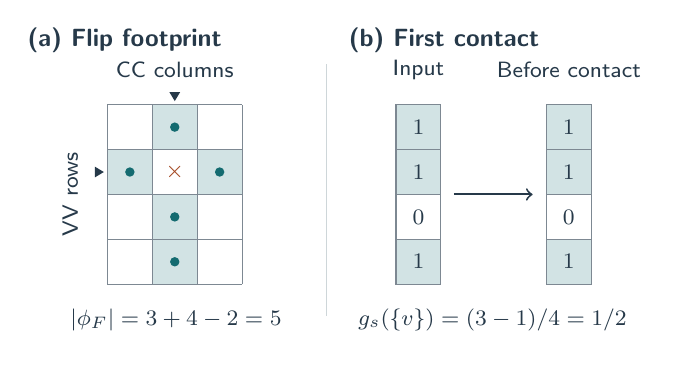
\begin{tikzpicture}[x=1cm,y=1cm,plot text]
  \node[panel title] at (0,3.72) {(a) Flip footprint};
  \node[panel title] at (4.08,3.72) {(b) First contact};
  \draw[graphgrid] (3.80,.22)--(3.80,3.42);
  \begin{scope}[shift={(1.02,.62)},x=.57cm,y=.57cm]
    \foreach \col/\row in {0/2,2/2,1/0,1/1,1/3}{
      \fill[graphteal!19] (\col,\row) rectangle ++(1,1);
      \fill[graphteal] (\col+.5,\row+.5) circle[radius=1.7pt];
    }
    \draw[graphink!60,line width=.4pt] (0,0) grid[step=.57cm] (3,4);
    \node[text=graphrust,inner sep=0pt] at (1.5,2.5) {$\times$};
    \fill[graphink] (-.28,2.38)--(-.28,2.62)--(-.08,2.5)--cycle;
    \fill[graphink] (1.38,4.28)--(1.62,4.28)--(1.5,4.08)--cycle;
    \node at (1.5,4.77) {CC columns};
    \node[rotate=90] at (-.83,2) {VV rows};
  \end{scope}
  \node at (1.89,.17) {$|\phi_F|=3+4-2=5$};
  \foreach \xx/\stage in {4.97/Input,6.88/Before contact}{
    \node at (\xx,3.34) {\stage};
    \begin{scope}[shift={(\xx,.62)},x=.57cm,y=.57cm]
      \foreach \row/\bit in {0/1,1/0,2/1,3/1}{
        \ifnum\bit=1
          \fill[graphteal!19] (-.5,\row) rectangle ++(1,1);
        \fi
        \draw[graphink!60,line width=.4pt] (-.5,\row) rectangle ++(1,1);
        \node[inner sep=0pt] at (0,\row+.5) {$\bit$};
      }
    \end{scope}
  }
  \draw[->,graphink,line width=.7pt] (5.42,1.76)--(6.42,1.76);
  \node at (5.91,.17) {$g_s(\{v\})=(3-1)/4=1/2$};
\end{tikzpicture}
\caption{Checks of a $(3,4)$ generator. (a) Selecting $x$ VV rows and
$y$ CC columns changes $3x+4y-2xy$ checks. Dots mark the footprint
of one row and one column. Their intersection cancels.
(b) An isolated CC fault $v$ has one inverted readout ($t_v=1$).
The three lit checks keep its singleton score at $1/2$ until first contact.
In a physically accepted history at $0<\beta\le1/4$, the first winner
touching $\psi_v$ thus scores at least $1/2$ on at least three checks.
Its integer syndrome decrease is at least two (Lemma~\ref{lem:first-contact}(b)).}
\label{fig:hgp-contact}
\end{figure}

Canonical recomposition (Theorem~\ref{thm:recomp}) holds for any fixed
finite family of distinct nonempty actions with nonempty footprints.
For the density bound of Proposition~\ref{prop:density}(a) and the
complexity estimates, we take actions inside generator supports of
uniformly bounded weight and incidence, as in~\eqref{eq:FGLfamily}.

\paragraph{The rule.} Fix $\beta>0$ and a syndrome-independent total order $\prec$ on $\FF$. For a current syndrome $s$, the score is the decrease in syndrome weight per check in the footprint,
\begin{equation}\label{eq:score}
 g_s(F)=\frac{|s|-|s\oplus\phi_F|}{|\phi_F|}
       =\frac{2|s\cap\phi_F|-|\phi_F|}{|\phi_F|}.
\end{equation}
When $\FF$ is nonempty and the maximum score is at least $\beta$, SSF selects the $\prec$-first maximizer and updates $s\leftarrow s\oplus\phi_F$. Otherwise it stops. Every accepted update lowers the integer $|s|$ by at least one, so each execution is finite.

The original SSF rule normalizes the syndrome decrease by the flip
weight $|F|$~\cite[Sec.~3]{LTZ15}. FGL's noisy-syndrome rule admits any
action meeting its footprint threshold~\cite[Alg.~2]{FGL18}.
Stambler, Krishna and Beverland study the case in which
SSF stops with unsatisfied checks on finite products~\cite{SKB23}.

\paragraph{Transcript, correction and support.} The transcript $\tau=(F_1,\dots,F_T)$ keeps all occurrences, in order. The correction $C(s_0)$ is the XOR of the occurrences. The execution support is the typed union
\begin{equation}\label{eq:support}
Y(E,D)=\Bigl(E\cup\bigcup\nolimits_{t}F_t\Bigr)\sqcup D\ \subseteq\ V\sqcup C_X .
\end{equation}

\subsection{Noise and computational input}

\paragraph{Independent data and readout faults.} Dennis et al.\ model
data faults and faulty syndrome outcomes by independent flips with
separate rates over successive rounds~\cite{DKLP02}. In our one round,
the fault sets $E\subseteq V$ and $D\subseteq C_X$ have independent
Bernoulli bits with rates $p,q\in[0,1/2)$. Write $z_p=p/(1-p)$, $z_q=q/(1-q)$ and $B_0=(1-p)^n(1-q)^{|C_X|}$.

\paragraph{Residual characters.}
For a physical mask $u$ and the residual $R=E\oplus C(s_0)$, write
\begin{equation}\label{eq:character}
 h_u(E,D)=(-1)^{u\cdot R},\qquad \lambda_u=\mathbb E\,h_u(E,D).
\end{equation}
On $H_XR=0$, protected masks distinguish residual logical classes.
An unfiltered sign can also change when the physical syndrome is nonzero.

\paragraph{Sizes.} Write $m_X=|C_X|=ab$ for the number of measured
checks and $N=n+m_X$ for the number of data and check sites. Let $w_Z$ be the maximum weight of a row of $H_Z$ and $\Delta_X$ the maximum column weight of $H_X$. In~\eqref{eq:HXHZ}, $\Delta_X=B$. For fixed $(A,B)$ and a candidate family contained in generator supports, all local quantities are constants. There are then $O(N)$ candidates, and the sparse combinatorial description of the code and candidates has size $\Theta(N)$. This combinatorial size is distinct from the binary input length $\Lin$ of Definition~\ref{def:contract}.

\begin{definition}[Input and order]\label{def:contract}
The input comprises the sparse check and generator incidences, the
deduplicated candidates, a mask $u$, rational $\beta,p,q$ of bit
length at most $\bpar$, and a list or ranks for $\prec$. The total
binary length $\Lin$ includes the requested accuracy. Alternatively,
a uniform comparator of bit cost $\Tprec(N,\Lin)$ permits rank
preparation in $O(N\log N)\Tprec(N,\Lin)$ for fixed local degrees.
Subsequent calls use the same ranks.
\end{definition}

\subsection{The interaction graph and local histories}

For $v\in V$ let $\psi_v=H_Xe_v$, and for $c\in C_X$ let $\psi_c=\{c\}$. The static host $K$ is the graph on $V\sqcup C_X$ in which distinct $x,y$ are adjacent if either:
\begin{itemize}
\item[(K1)] some $F\in\FF$ has $\phi_F\cap\psi_x\neq\varnothing$ and $\phi_F\cap\psi_y\neq\varnothing$; or
\item[(K2)] some $F\in\FF$ contains $y$ and satisfies $\phi_F\cap\psi_x\neq\varnothing$, or the same holds with $x$ and $y$ exchanged.
\end{itemize}
For candidate families contained in generator supports with uniformly bounded weights and incidences, the degree $\Delta(K)$ is bounded by a constant. Two vertex sets are \emph{compatible} if they are disjoint and not adjacent in $K$.

\begin{definition}[Decorated polymers and marks]\label{def:polymer}
A \emph{valid decorated polymer} is a tuple $\gamma=(Y,E_Y,D_Y,\tau_Y)$ with the following properties:
\begin{itemize}
\item $K[Y]$ is connected and non-empty;
\item $E_Y\subseteq Y\cap V$ and $D_Y=Y\cap C_X$;
\item the complete decoder, run on $(E_Y,D_Y)$ with all other sites fault-free, has execution support exactly $Y$ and transcript $\tau_Y$.
\end{itemize}
Its residual is $R_\gamma=E_Y\oplus\bigoplus_{F\in\tau_Y}F$, taking the XOR over occurrences. Its weight is $w(\gamma)=z_p^{|E_Y|}z_q^{|D_Y|}$, and its mark is $m_u(\gamma)=(-1)^{u\cdot R_\gamma}$.
\end{definition}

\subsection{Physical filtering and the main theorem}
Write $S=S_X$ and $T=\ker H_X$. The physical acceptance probability
is $P_0=\Pr[R\in T]$ and the per-round silent-failure probability is
$P_{\rm sil}=\Pr[R\in T\setminus S]$. Their ratio
$Q_{\rm sil}=P_{\rm sil}/P_0$ is the failure probability conditional
on acceptance. The no-fault history gives $P_0\ge B_0>0$. An ideal
terminal measurement of the data in the computational basis yields
the physical check parities.

Define the physically filtered activities and their formal partitions by
\begin{equation}\label{eq:filtered-weights-definition}
\begin{split}
 W_{T,u}(Y)&=\sum_{\substack{\gamma:Y_\gamma=Y\\H_XR_\gamma=0}}
                  w(\gamma)m_u(\gamma),\\
 \Xi_{T,u}(J)&=\sum_{\substack{\Gamma\ \mathrm{compatible}\\Y\subseteq J\ (Y\in\Gamma)}}
                        \prod_{Y\in\Gamma}W_{T,u}(Y).
\end{split}
\end{equation}
Here $J$ denotes the vertex set of an induced subhost, the empty family
contributes $1$, and $W_T=W_{T,0}$, $\Xi_T=\Xi_{T,0}$; omit $J$ for
the full host. Lemma~\ref{lem:conditioned-gas} identifies these partitions
with the physical probabilities.

\begin{definition}[Filtered partition access]\label{def:filtered-access}
After the input and order preparation of Proposition~\ref{prop:oracle},
assume a uniform deterministic algorithm that, for every physical mask
$u$, induced subhost $J$ and rational $0<\zeta\le1$, approximates
$\Xi_{T,u}(J)$ to relative error $\zeta$ in
$\poly(N,\zeta^{-1},\Lin)$ bit time. It also certifies that these
partition functions are positive. The unmarked case is $u=0$.
Local bounds and algorithmic margins are fixed. Restricting to $J$
limits the allowed supports. All candidates still compete.
\end{definition}
Sufficient conditions for this access come from a bound on each weight
(Proposition~\ref{prop:filtered-criteria}), a budget on fault sources
(Proposition~\ref{prop:kp-filtered-compiler}), or an expansion in the
original faults (Corollary~\ref{cor:mixed-source-cumulants}).

\begin{theorem}[Relative approximation of physical silent failure]\label{thm:silent-conditioned}
Assume exact canonical recomposition, separation of check neighbourhoods
of compatible data supports, the effective oracle and order contract,
fixed local bounds, and Definition~\ref{def:filtered-access}. Let
$0<p<1/2$ and $0\le q<1/2$ be rational rates in that certified regime.
Suppose a verified $L\in T\setminus S$ of weight $w\ge1$ is supplied
or constructed in polynomial time. Then $P_0$, $Q_{\rm sil}$ and
$P_{\rm sil}$ admit deterministic relative $\varepsilon$-approximations,
$0<\varepsilon\le1$. The bit costs are
$\poly(N,\varepsilon^{-1},\Lin)$ for $P_0$, and
\begin{equation}\label{eq:silent-modular-cost}
 \poly(N,\varepsilon^{-1},1+z_p^{-w},\Lin)
\end{equation}
for the failure probabilities, plus order preparation once.
For full-row-rank HGP seeds with fixed degrees $A<B$, the FGL family,
a fixed admissible $p>0$ and a uniform filtered-access certificate,
\begin{equation}\label{eq:silent-hgp-cost}
 \exp[O(\sqrt n)]\poly(N,\varepsilon^{-1},\Lin)
\end{equation}
suffices. The rational $q$ may vary within that uniform certificate.
No bilateral expansion, distance lower bound, or constant lower bound
on $P_0$ is required. For varying $p$, retain
\eqref{eq:silent-modular-cost}. If $p=0$ or $T=S$, both failure
probabilities are zero and are returned exactly; $P_0$ is still computed
under the partition-access contract when requested.
\end{theorem}

Section~\ref{sec:conditioned} relates $\zeta$ to $\varepsilon$.
Appendix~\ref{app:probability-proofs} gives the error analysis and
Corollary~\ref{cor:short-witness} the polynomial bound for short witnesses.

\section{Reconstructing the SSF execution}\label{sec:block1}

To assign a partition weight to a proposed support, we must decide
whether SSF stays inside it. Kovalev, Dumer and Pryadko enumerate
connected qubit supports to find the distance of a quantum LDPC
code~\cite{KDP13}. Dumer, Kovalev and Pryadko split an undetectable
Pauli operator into irreducible factors to bound decoding
failure~\cite[Lemma~4]{DKP15}. For SSF the host $K$ also records which
sites can influence the choice of a flip. Rule (K1) joins any two sites
read by the same candidate, even if its action extends outside the
proposed support. Its readers in the support therefore lie in at most one
component. Rule (K2) attaches the winning action to that component.

\begin{lemma}[Visibility and attachment]\label{lem:visibility}
Let $Y_1,\ldots,Y_k$ be the components of $K[Y]$. Assign a binary
coefficient $b_v$ to each $v\in Y\cap V$, fix $D\subseteq Y\cap C_X$, and set
\[
 s_i=\bigoplus_{\substack{v\in Y_i\cap V\\b_v=1}}\psi_v
       \oplus(D\cap Y_i),\qquad s=\bigoplus_i s_i.
\]
The readers of $H\in\FF$ in $Y$ form the set
$\mathcal R_H(Y)=\{x\in Y:\psi_x\cap\phi_H\ne\varnothing\}$.
If this set is nonempty, it lies in one component $Y_i$, and
\[
 s\cap\phi_H=s_i\cap\phi_H,\qquad g_s(H)=g_{s_i}(H).
\]
If it is empty, $g_s(H)=-1$. Moreover, for an actual execution with final
support $Y$, every selected action is contained in a single component of
$K[Y]$.
\end{lemma}

\begin{theorem}[Canonical recomposition]\label{thm:recomp}
Let $\FF$ be any fixed finite family of distinct non-empty sets with
non-empty footprints, let $\beta>0$, and fix a total order $\prec$ on
$\FF$ independent of the syndrome.
\begin{enumerate}
\item[(i)] \emph{Restriction.} For every history $(E,D)$, let
$Y_1,\ldots,Y_k$ be the components of $K[Y(E,D)]$. The complete decoder
run on $(E\cap Y_i,D\cap Y_i)$ produces exactly the subsequence of global
actions contained in $Y_i$, with the same occurrences and order. It stops
when that subsequence ends, and its execution support is $Y_i$.
Every selected global action is contained in a single component.
\item[(ii)] \emph{Inverse.} For any compatible family of valid decorated
polymers $\gamma_1,\ldots,\gamma_k$, the history obtained by taking the
unions of their fault sets executes the unique canonical interleaving of
their transcripts. Its support has exactly their supports as components,
and restricting it returns the original decorations.
\item[(iii)] \emph{Bijection and factorization.} Histories are in bijection
with compatible families of valid decorated polymers, including the
empty family. Under this bijection,
\[
 R=\bigoplus_i R_{\gamma_i},\qquad
 h_u(E,D)=\prod_i m_u(\gamma_i).
\]
\end{enumerate}
\end{theorem}

At each step the eligible candidates split by the component they read.
Comparing the local winners by score and then by $\prec$ gives the next
global flip (Fig.~\ref{fig:recomposition}). This comparison also detects
when every component has stopped (Appendix~\ref{app:execution-proofs}).

\begin{figure}[!htb]
\centering
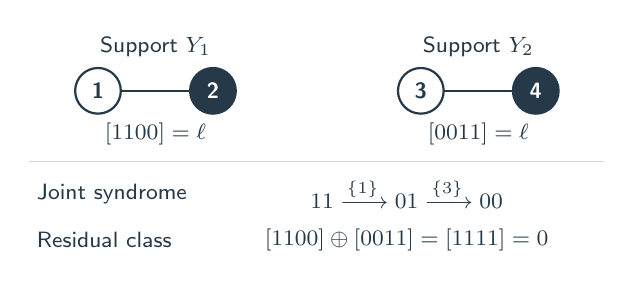
\begin{tikzpicture}[x=1cm,y=1cm,plot text,
    site/.style={circle,draw=graphink,line width=.8pt,minimum size=5.8mm,
                 inner sep=0pt,font=\sffamily\bfseries\footnotesize},
    flipped/.style={site,fill=graphink,text=white},
    selected/.style={site,fill=white,text=graphink}]
  \node at (1.65,2.48) {Support $Y_1$};
  \node at (5.75,2.48) {Support $Y_2$};
  \draw[graphink,line width=.9pt] (.92,1.92)--(2.38,1.92)
                                    (5.02,1.92)--(6.48,1.92);
  \node[selected] at (.92,1.92) {1};
  \node[flipped] at (2.38,1.92) {2};
  \node[selected] at (5.02,1.92) {3};
  \node[flipped] at (6.48,1.92) {4};
  \node at (1.65,1.37) {$[1100]=\ell$};
  \node at (5.75,1.37) {$[0011]=\ell$};
  \draw[graphgrid] (.05,1.02)--(7.34,1.02);
  \node[anchor=west] at (.02,.61) {Joint syndrome};
  \node at (4.84,.62) {$11\xrightarrow{\{1\}}01\xrightarrow{\{3\}}00$};
  \node[anchor=west] at (.02,.03) {Residual class};
  \node at (4.84,.03) {$[1100]\oplus[0011]=[1111]=0$};
\end{tikzpicture}
\caption{Exact recomposition in a four-qubit CSS example. The two
$Z$ checks measure parity on pairs $(1,2)$ and $(3,4)$, and
$S_X=\langle1111\rangle$. Filled sites are the initial data faults,
and open sites are the selected flips. There are no readout faults.
The candidates are the four singletons, with $\beta=1$ and ties in
increasing site order.
Silent failure occurs exactly when the initial fault bits at sites
2 and 4 differ. Adding fault 4 to $\{2\}$ changes the residual class
from $\ell$ to $[1111]=0$. The eight failing patterns form two
connected components of four under single-site changes that preserve
failure.}
\label{fig:recomposition}
\end{figure}

This argument gives an exact way to evaluate a weight. For a proposed
connected support $Y$, enumerate its possible data sources, fix its
check sources, and run the complete decoder with all other sites
fault-free. Reject the assignment if the global winner ever leaves $Y$
or the final support differs from $Y$. Sum the weights of the remaining
assignments with their residual signs. For fixed local parameters, the
work is exponential in $|Y|$ and polynomial in the local arithmetic
and index lengths (Proposition~\ref{prop:oracle}).

SSF implementations use Gray-code updates~\cite{GK19} and skip
generators whose rectangles contain no unsatisfied checks~\cite[App.~D]{SKB23}.
The code accompanying Berthusen and Gottesman~\cite{BG24} enumerates
column subsets and, for each one, sorts the rows by their gain in
syndrome weight. For the footprint score~\eqref{eq:score} and FGL
eligibility test, Proposition~\ref{prop:implicit-competition} needs only
the chosen active columns and the counts of other chosen columns and
rows. Its representative preserves the global winner, including ties,
for the orders specified there.

\section{Conditional logical failure}\label{sec:conditioned}

Conditioning on measured syndromes yields logical and abort thresholds
for surface-code postselection~\cite{EWB25}. For a finite square toric
code with independent bit flips, English et al.\ compute the failure
probability at zero input syndrome from four Ising partition
functions~\cite[Sec.~III]{ERBDW26}.

For SSF we test the physical syndrome after correction. On a regular
product with full FGL, two data qubits sharing a check are visible to
either singleton and therefore adjacent in $K$. Compatible components
thus have disjoint data-check neighbourhoods, and physical acceptance
holds exactly when each component passes. Their logical signs
$(-1)^{u\cdot R_i}$ multiply. Two copies of the same logical class
cancel, as in Fig.~\ref{fig:recomposition}.

By Lemma~\ref{lem:conditioned-gas}, $P_0=B_0\Xi_T$ and
$\Xi_{T,u}/\Xi_T$ is the mean of $(-1)^{u\cdot R}$ conditional on
$R\in T=\ker H_X$.
Let $\mathcal M$ be a set of representatives for $S_X^\perp/T^\perp$.
The corresponding characters of $T/S_X$ average to one on the
trivial logical class and to zero on each other class. Hence
\[
 Q_{\rm sil}=\frac{1}{|\mathcal M|}\sum_{u\in\mathcal M}
              \left(1-\frac{\Xi_{T,u}}{\Xi_T}\right).
\]
Multiplying by $P_0$ gives the per-round probability $P_{\rm sil}$.
An explicit small-bias multiset approximates the character average
with polynomially many masks~\cite{NN93,AGHP92}.

\paragraph{Pairing by a logical operator.}
Fix $L\in T\setminus S_X$ of weight $w$. Pair $(E,D)$ with
$(E\oplus L,D)$. Both histories have the same observed syndrome,
correction and physical acceptance. Within an accepted pair the
residual classes differ by $L$, so at least one member fails.
If the smaller mass is at least $\kappa$ times the larger
($0<\kappa\le1$) in each pair of positive total mass, the silent
fraction of the accepted mass is at least $\kappa/(1+\kappa)$.
For Bernoulli data faults one can take $\kappa=z_p^w$,
as shown in~\eqref{eq:conditional-witness}. For full-row-rank seeds
of degrees $A<B$, Lemma~\ref{lem:total-witness} gives $w\le a\le\sqrt n$.
The same syndrome ambiguity enters exclusive decoding~\cite{SBB24}
and counts of minimum-weight failures~\cite[Sec.~4.3]{BCCY25}.

For any certified $0<\ell\le Q_{\rm sil}$, partition tolerances of
order $\varepsilon\ell$ suffice for a relative $\varepsilon$-estimate
of $P_{\rm sil}$. A shorter witness or a larger lower bound from a
counted failure sector reduces the required precision.
Appendix~\ref{app:probability-proofs} gives the bit cost.

Partition functions also describe
logical-class probabilities under correlated Pauli noise~\cite{CF21}.
At fixed surface-code syndrome, maximum-likelihood decoding with
independent bit and phase flips and perfect readout takes $O(n^2)$
time~\cite{BSV14}. Other approaches average coset probabilities over
syndromes to evaluate a prescribed decoder~\cite{CGLW24}, certify a
maximum-likelihood decision from class weights~\cite{Kri26}, or estimate
the risk of a correction from the decoder's soft output~\cite{MPP24}.

\section{Certified noise rates}\label{sec:certificates}

\subsection{Independent data and readout faults}
An initially fully lit data fault has singleton score one until an
action first touches an incident check. Every winner through that
contact extinguishes its entire footprint, so these footprints are
disjoint. For regular self-products with full FGL, $1\le A\le B$,
$B\ge2$ and $0<\beta\le1$, Lemma~\ref{lem:first-contact}(a) marks
each distinct first-contact action once for a singleton and twice
for a larger flip. A source group with $j$ marks thus accounts for
at least $\lceil j\min(2A,A+B-2)/2\rceil$ distinct initially lit
checks turned off. The bound allows four-cycles.

Part~(b) also covers a data fault $v$ isolated in the data-fault
graph $K[E]$ when $t_v$ of its $n_v$ incident checks have flipped
readouts. On a physically accepted history, if $A\ge3$ and
$0<\beta\le1/B$, the first action touching those checks lowers the
syndrome weight by at least $\max\{1,\lceil A b_v/n_v\rceil\}$,
where $b_v=n_v-2t_v$. For $B\le A+2$ the decrease is at least $b_v$.
This includes $(3,4)$ (Fig.~\ref{fig:hgp-contact}(b)) and $(17,18)$. The examples at
$(7,10)$ and $(8,11)$ in Appendix~\ref{app:contact-examples} show
how a preceding flip that lights new checks can reduce the decrease
at first contact.

Single-shot recovery bounds the residual noise after a noisy
round~\cite{Bombin15}. On sufficiently expanding products FGL prove
such a bound under local stochastic faults, which can be
correlated~\cite[Thm.~2]{FGL18}.

Since each flip lowers the syndrome weight by at least one, subtracting
the drops at distinct first contacts from the initial weight bounds the
number of flips far from the data faults. Under independent Bernoulli
noise we bound the total weight of groups containing a fixed source,
over all group sizes and uniformly in seed size. For $(3,4)$ the
tail of the filtered log partition after total source degree $M$,
counting repetitions, is at most $Ne^{-0.015(M+1)}$ throughout the
Bernoulli rectangles of Table~\ref{tab:fibre-34}. These rectangles
and the $(17,18)$ rectangle~\eqref{eq:mixed-source-region} use full FGL
competition at $\beta=1/100$ and a fixed tie order
(Appendices~\ref{app:mixed-source-cumulants} and~\ref{app:low-degree}).
For one readout-only $(3,4)$ subhost the filtered partition is positive
for $0\le q<1$. Its nearest zero satisfies $-0.097080<q_*<-0.097079$,
so its logarithm has Taylor radius $|q_*|$ about $q=0$.

The $(3,4)$ degree pair also appears in analytic bounds for
maximum-likelihood decoding of products of random Gallager seeds
under data noise~\cite{KPDP18}, in simulations of hybrid belief
propagation and SSF~\cite{GGKL21}, and in proposed thin-planar and
reconfigurable atom-array layouts~\cite{TDB22,Xu24}. At the Bernoulli
endpoint $(p,q)=(10^{-6},10^{-4})$, consider the 225- and 900-qubit
codes of Section~\ref{sec:marked-volumes}. For $10\%$ relative error
in $P_{\rm sil}$, \eqref{eq:relative-error-budget} gives partition
tolerance $\zeta=\ell/1280$ for any certified $0<\ell\le Q_{\rm sil}$.
Requiring a log tail of at most $\zeta/4$ gives sufficient cutoffs
$M=6\,482$ and $6\,575$, respectively, with the weight-six witness. Using
just the mass of the two-data, one-readout sector gives $M=3\,028$
and $3\,057$.

\subsection{One round of syndrome extraction}\label{sec:circuit}
A single circuit fault can change both a data qubit and several
readouts. In one round of $Z$-syndrome extraction, each check has a
target ancilla coupled to its data controls on a fixed layered CNOT
schedule and measured once. At operation rate $r_c$, faulty one- and
two-qubit operations apply uniform nonidentity Pauli errors, as in
Stephens~\cite[Sec.~V.C]{Stephens14}. An independent classical flip
of rate $r_m$ follows the one-qubit Pauli channel at readout.

For a repetition-code circuit, Vodola et al.\ derive exact rates for
data errors, readout errors and a joint data--readout error
\cite[Eqs.~(6)--(9)]{VRKM22}. For LDPC extraction circuits, Pattison,
Krishna and Preskill bound the joint errors on data and ancillas per
round by a locally decaying distribution~\cite[Def.~2.5 and Sec.~5.1]{PKP25}.

For any binary CSS code in this model, Proposition~\ref{prop:wire-check-fibres}
gives independent wire labels $(\epsilon_v,\delta_v)$ and check bits
$B_j$. Each wire keeps its final data parity and readout offsets together.
With $E_X=(\epsilon_v)_v$ and $B=(B_j)_j$, SSF sees
$s=H_XE_X\oplus B\oplus\bigoplus_v\delta_v$.
Figure~\ref{fig:circuit-fibres} follows a single wire fault through this sum.

\begin{figure}[!htb]
\centering
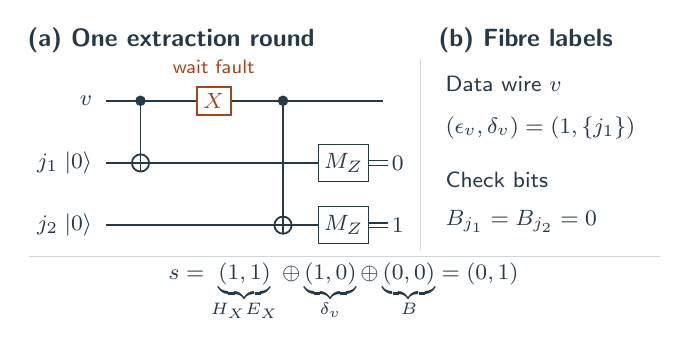
\begin{tikzpicture}[x=1cm,y=1cm,plot text,
    wire/.style={draw=graphink,line width=.65pt},
    meter/.style={draw=graphink,fill=white,inner sep=2pt,
                  minimum height=4.7mm}]
  \node[panel title] at (0,3.13) {(a) One extraction round};
  \node[panel title] at (5.22,3.13) {(b) Fibre labels};
  \draw[graphgrid] (5.00,.46)--(5.00,2.89);
  \node[anchor=east] at (.95,2.36) {$v$};
  \node[anchor=east] at (.95,1.57) {$j_1\;\lvert0\rangle$};
  \node[anchor=east] at (.95,.78) {$j_2\;\lvert0\rangle$};
  \draw[wire] (1.00,2.36)--(4.52,2.36);
  \foreach \cy in {1.57,.78}{
    \draw[wire] (1.00,\cy)--(4.02,\cy);
    \draw[graphink,line width=.55pt]
        (4.02,\cy+.030)--(4.58,\cy+.030)
        (4.02,\cy-.030)--(4.58,\cy-.030);
    \node[meter] at (4.02,\cy) {$M_Z$};
  }
  \foreach \gx/\cy in {1.44/1.57,3.25/.78}{
    \draw[wire] (\gx,2.36)--(\gx,\cy);
    \fill[graphink] (\gx,2.36) circle[radius=1.9pt];
    \draw[wire,fill=white] (\gx,\cy) circle[radius=3.1pt];
    \draw[wire] (\gx-.102,\cy)--(\gx+.102,\cy)
                (\gx,\cy-.102)--(\gx,\cy+.102);
  }
  \node[draw=graphrust,text=graphrust,fill=white,
        line width=.75pt,inner sep=2.3pt] at (2.37,2.36) {$X$};
  \node[font=\sffamily\scriptsize,text=graphrust] at (2.37,2.79) {wait fault};
  \node[anchor=west,inner sep=1pt] at (4.59,1.57) {$0$};
  \node[anchor=west,inner sep=1pt] at (4.59,.78) {$1$};
  \node[anchor=west] at (5.19,2.57) {Data wire $v$};
  \node[anchor=west] at (5.19,2.02) {$(\epsilon_v,\delta_v)=(1,\{j_1\})$};
  \node[anchor=west] at (5.19,1.36) {Check bits};
  \node[anchor=west] at (5.19,.83) {$B_{j_1}=B_{j_2}=0$};
  \draw[graphgrid] (.03,.38)--(8.04,.38);
  \node at (4.02,-.07)
    {$s=\underbrace{(1,1)}_{H_XE_X}\oplus
          \underbrace{(1,0)}_{\delta_v}\oplus
          \underbrace{(0,0)}_{B}=(0,1)$};
\end{tikzpicture}
\caption{Wire and check fibres in one round of $Z$ extraction
(Proposition~\ref{prop:wire-check-fibres}). The data wire touches two
checks. A single $X$ fault during the intervening wait reaches only the
second ancilla. The wire label records both the
final data error and the discrepancy at the first check. Reversing the
two CNOTs moves the discrepancy to $j_2$. The independent fibre laws
are combined before SSF and physical filtering.}
\label{fig:circuit-fibres}
\end{figure}

Corollary~\ref{cor:fibre-transfer} transfers a Bernoulli certificate
with source budgets $x_D,x_M$ if two conditions hold. On every admitted
subhost throughout the noise rectangle the nonzero-to-zero odds satisfy
$g_{D,v}\le x_D$ and $g_{M,j}\le x_M$, as can be tested
by~\eqref{eq:fibre-odds}. The rooted counts must cover every admissible
wire label at the original tilt, with the same support bound and
coefficient access.

When primitive histories recompose exactly and physical acceptance
factors over components (Proposition~\ref{prop:circ-recomp}),
uniform effective relative access to the
filtered marked partitions on induced subhosts gives a deterministic
relative estimate of $P_0$. If a verified logical operator in the
initial or final wait layer gives $\kappa_L>0$ in~\eqref{eq:circ-witness},
Theorem~\ref{thm:circ-relative} gives such estimates for $Q_{\rm sil}$
and $P_{\rm sil}$ as well.

For $(3,4)$, direct transfer of $(p,q)=(3.2\cdot10^{-7},10^{-3})$
certifies $(r_c,r_m)=(4.2\cdot10^{-8},10^{-3})$. The position of a
wire fault determines which readouts it can affect. Accounting for the
gate order gives the larger rectangles in Table~\ref{tab:fibre-34},
among them $(r_c,r_m)=(2\cdot10^{-7},10^{-5})$ with VV first, where
the readout odds exceed the direct-transfer budget
(Appendix~\ref{app:fibre-transfer}).

\begin{table}[!htb]
\centering\small
\caption{Sufficient input rates for uniform partition access on binary $(3,4)$
self-products with full FGL at $\beta=1/100$. Each endpoint covers the corresponding rectangle from
zero, including seeds with four-cycles. The Bernoulli endpoints use tilt $0.015$. In the circuit,
$\lambda_{\rm c}$ gives a logarithmic tail bounded by
$(n+m_X)e^{-\lambda_{\rm c}(k+1)}$ after total fibre degree $k$.
All circuit rows use the ten layers of Appendix~\ref{app:circuit}.
VV first assigns colours to the four VV incidences of each check before
its three CC incidences. Gates execute in colour order. The last column
allows any fixed ordering of the data columns in this construction.
The last two rows share the Bernoulli endpoint.}
\label{tab:fibre-34}
\smallskip
\begin{tabular}{@{}lrrcc@{}}
\toprule
 & & & \multicolumn{2}{c}{$10^{7}r_{c,0}$}\\
\cmidrule(l){4-5}
$q_0=r_{m,0}$ & $10^6p_0$ & $\lambda_{\rm c}$ & VV first & Any order\\
\midrule
$10^{-3}$ & 0.540 & 0.015  & 1.005 & 0.918\\
$10^{-4}$ & 1.00  & 0.015  & 1.85  & 1.68\\
$10^{-5}$ & 1.06  & 0.015  & 1.975 & 1.781\\
$10^{-5}$ & \textit{same} & 0.0025 & 2.000 & 1.803\\
\bottomrule
\end{tabular}
\end{table}

\section{Precision on the affine F17 code}\label{sec:f17}

Section~\ref{sec:conditioned} relates the precision of a partition
query to a lower bound on $Q_{\rm sil}$. On F17 we can compare two such
bounds at the same Bernoulli rates. Its seed is the binary point--line
incidence matrix of the affine plane over $\mathbb F_{17}$, with $289$
rows and $306$ columns. Each line contains $17$ points and each point
lies on $18$ lines, giving column and row weights $(17,18)$. The
self-product encodes $289$ logical qubits in $177\,157$ data qubits
with $88\,434$ measured checks.

Fix the family-wide Bernoulli endpoint
$(p,q)=(5\cdot10^{-33},2\cdot10^{-11})$. The union of two parallel
classes is an even set of affine lines~\cite[Sec.~4]{MJ04}.
Placed on a suitable data row it gives a weight-$34$ logical
operator. Pairing histories with this operator gives
$Q_{\rm sil}\ge 5.82\cdot10^{-1099}$.
Stambler et al.\ reduce SSF to classical bit flipping when the
syndrome lies in one product line~\cite[Lemma~1]{SKB23}.
All $18$ parallel classes on a data row produce the same syndrome.
By the FGL row reduction in Appendix~\ref{app:f17algebra}, the first
selected line determines which class SSF removes. For every fixed tie order, $17$ of the $18$ initial classes
therefore leave a nontrivial logical error. Summing these configurations
over the rows gives $P_{\rm sil}\ge 3.96\cdot10^{-546}$, also a lower
bound on $Q_{\rm sil}$.

For a target relative error of $10\%$, the logical witness gives a
sufficient cutoff of $253\,000$ in total source degree. Counting the
parallel-class failures lowers this cutoff to $126\,000$ with the same
convergence bound (Appendix~\ref{app:f17-orders}). A single decoder
step illustrates the cost of evaluating a connected weight. For one parallel-class input,
about $1.2\cdot10^{14}$ candidates read the initial syndrome. The
implicit comparison in Proposition~\ref{prop:implicit-competition}
finds the global winner by evaluating $2\,221\,254$ representatives.

Under circuit noise the whole $(17,18)$ family admits $r_c=2\cdot10^{-35}$
at $r_m=2\cdot10^{-11}$. Using the number of locations in this particular
affine circuit gives $r_c=5\cdot10^{-33}$ at the same readout rate
(Appendix~\ref{app:fibre-transfer}). At that endpoint a sector for the
specified schedule and tie order contributes at least
$1.02\cdot10^{-499}$ to $P_{\rm sil}$ (Appendix~\ref{app:finite-sector}).

\section{Finite estimates of silent failure}\label{sec:finite-estimates}

We bound the mass of silent failures inside and outside a finite
count. We group configurations by fault counts on the affine codes
and by connected SSF components on strips. Given $0<L\le P_{\rm sil}\le U$, we report
the harmonic estimate $2LU/(L+U)$. Its worst relative error on the
interval is $(U-L)/(U+L)$ (Lemma~\ref{lem:harmonic-point}). For sampled
endpoints this statement applies on the joint coverage event.

\subsection{Fault sectors on 225 and 900 qubits}\label{sec:marked-volumes}
\begin{figure*}[!t]
\centering
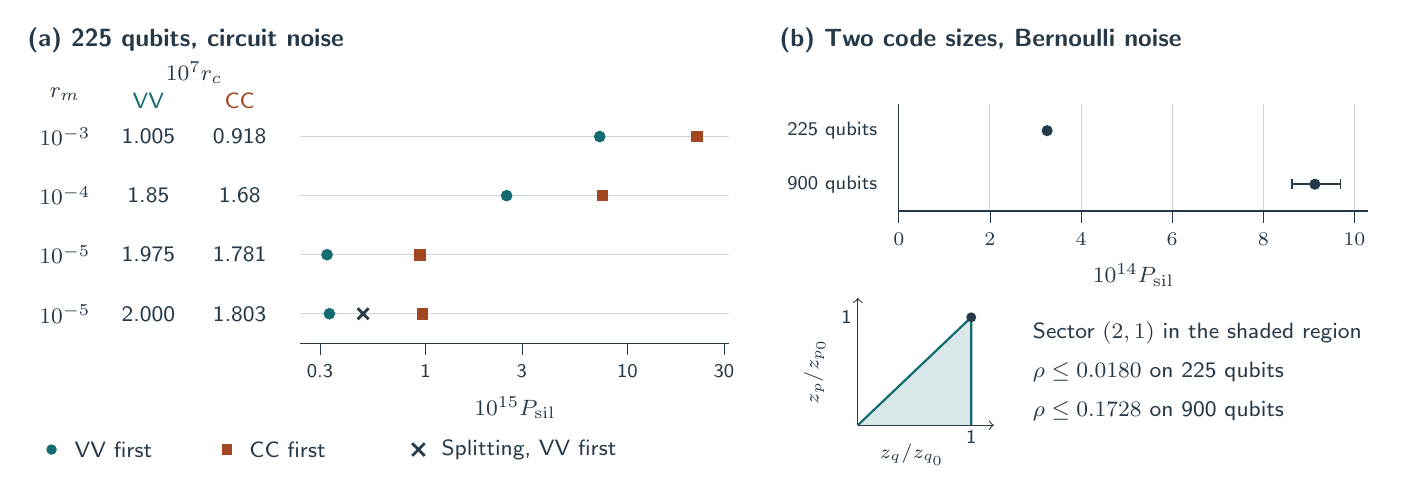
\begin{tikzpicture}[x=1cm,y=1cm,plot text]
  \node[panel title] at (0,5.05) {(a) 225 qubits, circuit noise};
  \node[panel title] at (9.55,5.05) {(b) Two code sizes, Bernoulli noise};
  \node at (.48,4.36) {$r_m$};
  \node at (2.12,4.64) {$10^7 r_c$};
  \node[text=graphteal] at (1.54,4.28) {VV};
  \node[text=graphrust] at (2.70,4.28) {CC};
  \foreach \row/\power/\vv/\cc in {4/-3/1.005/0.918,3/-4/1.85/1.68,
                                      2/-5/1.975/1.781,1/-5/2.000/1.803}{
    \draw[graphgrid,line width=.3pt]
      (3.47,{1.20+(\row-.5)*.75})--(8.92,{1.20+(\row-.5)*.75});
    \node at (.48,{1.20+(\row-.5)*.75}) {$10^{\power}$};
    \node at (1.54,{1.20+(\row-.5)*.75}) {\vv};
    \node at (2.70,{1.20+(\row-.5)*.75}) {\cc};
  }
  \begin{semilogxaxis}[paper axis,at={(3.47cm,1.20cm)},anchor=south west,
    width=5.45cm,height=3cm,xmin=.24,xmax=32,ymin=.5,ymax=4.5,
    xtick={.3,1,3,10,30},xticklabels={0.3,1,3,10,30},
    ytick={1,2,3,4},yticklabels=\empty,axis y line=none,
    axis x line*=bottom,ymajorgrids,xlabel={$10^{15}P_{\rm sil}$},
    tick label style={font=\sffamily\scriptsize}]
    % Source: the eight interval rows in piloto_HGP_225_esquinas_20261124.json.
    \addplot+[only marks,graphteal,mark=*,mark size=1.9pt,
      mark options={solid,fill=graphteal,draw=graphteal},
      error bars/.cd,x dir=both,x explicit]
      table[x=est,y=row,x error minus expr=\thisrow{est}-\thisrow{lo},
                         x error plus expr=\thisrow{hi}-\thisrow{est}] {
        row est          lo           hi
        4    7.287649080  7.265146024  7.310291972
        3    2.521498433  2.519747621  2.523251681
        2    0.325370226  0.325116839  0.325624008
        1    0.334223095  0.333938803  0.334507872
      };
    \addplot+[only marks,graphrust,mark=square*,mark size=1.9pt,
      mark options={solid,fill=graphrust,draw=graphrust},
      error bars/.cd,x dir=both,x explicit]
      table[x=est,y=row,x error minus expr=\thisrow{est}-\thisrow{lo},
                         x error plus expr=\thisrow{hi}-\thisrow{est}] {
        row est           lo            hi
        4   22.020399255 21.968158744 22.072888816
        3    7.524380506  7.520585695  7.528179148
        2    0.942045731  0.941547001  0.942544991
        1    0.966848229  0.966286195  0.967410917
      };
    \addplot[only marks,graphink,mark=x,mark size=2.8pt,line width=1pt]
      coordinates {(.4912342963,1)};
  \end{semilogxaxis}
  \begin{scope}[yshift=-2.5mm]
  \fill[graphteal] (.31,.10) circle (1.9pt);
  \node[anchor=west] at (.48,.10) {VV first};
  \fill[graphrust] (2.47,.035) rectangle ++(.13,.13);
  \node[anchor=west] at (2.70,.10) {CC first};
  \draw[graphink,line width=1pt] (4.89,.02)--(5.05,.18) (4.89,.18)--(5.05,.02);
  \node[anchor=west] at (5.14,.10) {Splitting, VV first};
  \end{scope}

  \begin{axis}[paper axis,at={(11.07cm,2.88cm)},anchor=south west,
    width=5.96cm,height=1.36cm,xmin=0,xmax=10.3,ymin=.5,ymax=2.5,
    xtick={0,2,4,6,8,10},ytick={1,2},yticklabels={900 qubits,225 qubits},
    axis x line*=bottom,axis y line*=left,ytick style={draw=none},
    xmajorgrids,xlabel={$10^{14}P_{\rm sil}$}]
    % Source: the cold-start sector calculation on both seeds (Table 2).
    \addplot+[only marks,graphink,mark=*,mark size=1.8pt,
      mark options={solid,fill=graphink,draw=graphink},
      error bars/.cd,x dir=both,x explicit,error bar style={line width=.9pt}]
      table[x=est,y=row,x error minus expr=\thisrow{est}-\thisrow{lo},
                          x error plus expr=\thisrow{hi}-\thisrow{est}] {
        row est          lo           hi
        2    3.256556360  3.240091581  3.273189328
        1    9.132409924  8.630394140  9.696435579
      };
  \end{axis}
  \begin{scope}[shift={(10.55cm,.16cm)},x=1.44cm,y=1.37cm,font=\sffamily\scriptsize]
    \fill[graphteal!16] (0,0)--(1,0)--(1,1)--cycle;
    \draw[graphteal,line width=.8pt] (0,0)--(1,1)--(1,0);
    \draw[graphink,->] (0,0)--(1.20,0);
    \draw[graphink,->] (0,0)--(0,1.18);
    \fill[graphink] (1,1) circle (1.8pt);
    \node[anchor=north,inner sep=2pt] at (1,0) {1};
    \node[anchor=east,inner sep=2pt] at (0,1) {1};
    \node at (.48,-.27) {$z_q/z_{q_0}$};
    \node[rotate=90] at (-.38,.50) {$z_p/z_{p_0}$};
  \end{scope}
  \node[anchor=west] at (12.65,1.33) {Sector $(2,1)$ in the shaded region};
  \node[anchor=west] at (12.65,.83) {$\rho\le 0.0180$ on 225 qubits};
  \node[anchor=west] at (12.65,.34) {$\rho\le 0.1728$ on 900 qubits};
\end{tikzpicture}
\caption{Silent failure on the affine code and its lift. (a) Each pair
shares a readout rate and uses the two operation rates at left. The
stratified intervals are narrower than the symbols and have joint
coverage above $98.54\%$ under independent trials within each stratum.
The cross is the splitting point estimate at the last VV-first setting,
whose stratified interval is $[3.33938,3.34508]\cdot10^{-16}$.
(b) Both codes have $d_X=6$. The dots and whiskers give the harmonic
estimates and deterministic intervals at $(p_0,q_0)=(10^{-6},10^{-4})$.
This point is the filled corner of the shaded region
$0<z_p/z_{p_0}\le z_q/z_{q_0}\le1$, with $z_x=x/(1-x)$. There
$P_{\rm sil}=T_{21}(1+\rho)$ by Corollary~\ref{cor:regional-sector}.}
\label{fig:affine-estimates}
\end{figure*}

The binary incidence matrix of the affine plane over $\mathbb F_3$ and
its connected two-sheet lift give the $[[225,9,6]]$ and $[[900,36,6]]$
products, respectively. The first also appears in studies of sliding-window
BP-OSD~\cite[Fig.~5]{QUITS25} and postselection~\cite[Fig.~5]{LEB26}.
At $(p,q)=(10^{-6},10^{-4})$ we use the full FGL family at
$\beta=1/100$. Ties favour the larger action, then the smaller
physical bit mask.

A sector $(i,j)$ fixes the data and readout weights, as in split
data--syndrome enumerators~\cite[Sec.~V]{ALB20}. Fault-weight sectors
also occur in postselected trapped-ion experiments~\cite{Linke17}.
On both codes $(2,0)$ contains no silent failures. Exact counts in
$(2,1),(2,2),(3,0)$ give the lower endpoint, and bounds on the other
sectors and binomial tails give the upper one
(Appendix~\ref{app:two-volumes}). The dominant sector $(2,1)$ has
$324$ silent inputs on 225 qubits and $864$ among
$432\binom{900}{2}=174\,765\,600$ on 900.

\begin{table}[!htb]
\centering\small
\setlength{\tabcolsep}{3pt}
\caption{Deterministic intervals at $(p,q)=(10^{-6},10^{-4})$ using
the same sector calculation on both codes. The error bounds apply
to the harmonic estimates. Timings include
construction of decoder and orbit tables from the seed, with the
C++ decoder already compiled.}
\label{tab:two-volumes}
\smallskip
\begin{tabular}{@{}rrrr@{}}
\toprule
Qubits & Interval for $10^{14}P_{\rm sil}$ & Error & Time (s)\\
\midrule
225 & $[3.24009,3.27319]$ & $<0.51\%$ & 1.10\\
900 & $[8.63039,9.69644]$ & $<5.82\%$ & 32.79\\
\bottomrule
\end{tabular}
\end{table}

The two harmonic estimates are $3.25656\cdot10^{-14}$ and
$9.13241\cdot10^{-14}$ (Fig.~\ref{fig:affine-estimates}(b)). A
finer count on 225 qubits lowers the upper endpoint to
$3.2624\cdot10^{-14}$ (Table~\ref{tab:affine225-pilot}). The logical
distance constrains which fault sectors can contribute.

\begin{lemma}[Data faults and logical distance]\label{lem:data-fault-distance}
For the self-product of a full-row-rank $(3,4)$ seed, let $d_X=\min_{L\in\ker H_X\setminus S_X}|L|$.
Under the max-score FGL rule ($0<\beta\le1$), silent failure with $e=|E|\ge1$ data faults requires $d_X\le4e-2$ for any readout mask $D$. Two data faults therefore require $d_X\le6$.
\end{lemma}

\begin{corollary}[Regional sector bound]\label{cor:regional-sector}
For independent Bernoulli noise on the two codes above, let $C_{ij}$ count silent inputs with $i$ data and $j$ readout faults, $m=|C_X|$, and
$T_{21}=C_{21}p^2q(1-p)^{n-2}(1-q)^{m-1}$. Put $z_x=x/(1-x)$, $r=z_p/z_q$, $s=z_q$, and evaluate $r_0,s_0$ at $(p_0,q_0)=(10^{-6},10^{-4})$.
Throughout $0<r\le r_0$, $0<s\le s_0$, we have $P_{\rm sil}=T_{21}(1+\rho)$ with $0\le\rho\le\bar\rho$, where $\bar\rho=0.0180$ for 225 qubits and $0.1728$ for 900.
\end{corollary}

Throughout the region in Corollary~\ref{cor:regional-sector}, the
interval $[T_{21},(1+\bar\rho)T_{21}]$ gives a harmonic estimate with
relative error below $0.90\%$ on 225 qubits and $8\%$ on 900
(Appendix~\ref{app:sector-bounds}). At $q=0$, $T_{21}$ vanishes
and both codes have silent $(3,0)$ inputs.

At $(p,q)=(10^{-6},10^{-4})$, the $(2,1)$ sector accounts for
$98.23$--$98.92\%$ of $P_{\rm sil}$ on 225 qubits and
$85.26$--$95.81\%$ on 900, using $T_{21}$ and the intervals in
Tables~\ref{tab:affine225-pilot} and~\ref{tab:two-volumes}, respectively.
With an empty trace the residual equals $E$, so silent failure requires at
least $d_X=6$ data faults, whatever the readouts. A union bound over
six-qubit subsets gives $\Pr[\text{silent failure, empty trace}]
\le\binom{n}{6}p^6$. Dividing by the deterministic lower endpoints in
Table~\ref{tab:two-volumes}, the fraction of silent failures with at
least one SSF step exceeds $1-5.21\cdot10^{-12}$ on 225 qubits and
$1-8.42\cdot10^{-9}$ on 900.

\paragraph{Direct sampling.}
For $N_{\rm MC}$ independent full rounds the sample mean of the
silent-failure indicator has relative root-mean-square error
$\sqrt{(1-P_{\rm sil})/(N_{\rm MC}P_{\rm sil})}$. At the 900-qubit
point estimate, $5.82\%$ relative RMS error would require about
$3.23\cdot10^{15}$ rounds. A two-sided $95\%$ interval of that
relative half-width would require about $1.24\cdot10^{16}$ rounds
under the normal approximation.

\paragraph{Gate order on 225 qubits.}
For the circuit calculation we assign each entire CNOT to its data
wire in the joint response of Proposition~\ref{prop:wire-check-fibres}.
The check fibres contain the ancilla operations and readout flips.
In each of the four pairs in Fig.~\ref{fig:affine-estimates}(a), the
schedules share $r_m$ and CC first uses the lower, any-order $r_c$ of
Table~\ref{tab:fibre-34}. The CC-first estimate is $2.89$--$3.02$
times the VV-first estimate.

At $(r_c,r_m)=(2\cdot10^{-7},10^{-5})$ with VV first, the sector
estimate is $3.34223\cdot10^{-16}$ in $8.31$ s (median of three runs).
Splitting gives $4.91234\cdot10^{-16}$ in $161.91$ s. This is
$46.85$--$47.11\%$ above $P_{\rm sil}$ on the joint coverage event
for the eight stratified intervals (above $98.54\%$ under independent
trials within each stratum, Table~\ref{tab:affine225-pilot}). The wider,
deterministic interval contains the splitting estimate. At the final
level the split $\widehat R$ for the ratio was $6.03$.
Appendix~\ref{app:rare-methods} gives the transition counts and the
Bernoulli comparison within the $(2,1)$ stratum.

\subsection{Compatible histories on growing strips}\label{sec:strip-certificates}
The strips are planar surface codes formed from two open repetition
codes. Fixing one length at six and varying the other over $6,12,24,48$
gives $61$, $127$, $259$ and $523$ data qubits, respectively, with
one logical qubit in every strip.

\begin{figure}[!htb]
\centering
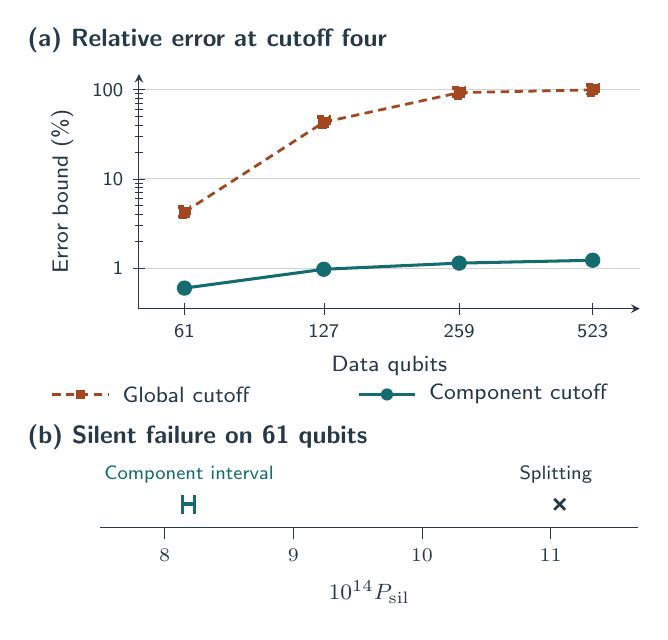
\begin{tikzpicture}[x=1cm,y=1cm,plot text]
  \node[panel title] at (0,5.88) {(a) Relative error at cutoff four};
  \begin{loglogaxis}[paper axis,at={(1.42cm,2.47cm)},anchor=south west,
    width=6.36cm,height=2.98cm,xmin=48,xmax=670,ymin=.35,ymax=150,
    xtick={61,127,259,523},xticklabels={61,127,259,523},
    ytick={1,10,100},yticklabels={1,10,100},axis lines=left,
    ymajorgrids,xlabel={Data qubits},ylabel={Error bound (\%)}]
    % Both columns use the same cell in results/circuit.json for each strip.
    \addplot[graphrust,densely dashed,line width=1pt,mark=square*,mark size=2pt]
      coordinates {(61,4.24041113) (127,43.16442866)
                   (259,92.63490117) (523,99.51258966)};
    \addplot[graphteal,line width=1.1pt,mark=*,mark size=2.2pt]
      coordinates {(61,0.59458862) (127,0.96712176)
                   (259,1.13372104) (523,1.22061913)};
  \end{loglogaxis}
  \draw[graphrust,line width=1pt,densely dashed] (.32,1.38)--(1.03,1.38);
  \fill[graphrust] (.62,1.32) rectangle ++(.12,.12);
  \node[anchor=west] at (1.09,1.38) {Global cutoff};
  \draw[graphteal,line width=1.1pt] (4.21,1.38)--(4.92,1.38);
  \fill[graphteal] (4.57,1.38) circle (2.2pt);
  \node[anchor=west] at (4.98,1.38) {Component cutoff};
  \node[panel title] at (0,.83) {(b) Silent failure on 61 qubits};
  \begin{axis}[paper axis,at={(.93cm,-.31cm)},anchor=south west,
    width=6.83cm,height=.82cm,xmin=7.50,xmax=11.68,ymin=0,ymax=1,
    xtick={8,9,10,11},ytick=\empty,axis y line=none,axis x line*=bottom,
    xlabel={$10^{14}P_{\rm sil}$}]
    \draw[graphteal,line width=1.3pt] (axis cs:8.13584002,.36)--(axis cs:8.23316829,.36);
    \draw[graphteal,line width=1pt] (axis cs:8.13584002,.21)--(axis cs:8.13584002,.51)
                                     (axis cs:8.23316829,.21)--(axis cs:8.23316829,.51);
    \node[font=\sffamily\scriptsize,text=graphteal,anchor=south] at (axis cs:8.19,.54)
      {Component interval};
    \addplot[graphink,only marks,mark=x,mark size=2.8pt,line width=1pt]
      coordinates {(11.0704,.36)};
    \node[font=\sffamily\scriptsize,text=graphink,anchor=south] at (axis cs:11.04,.54)
      {Splitting};
  \end{axis}
\end{tikzpicture}
\caption{Circuit noise at $r_c=r_m=10^{-5}$ on fixed-width strips.
(a) Each pair bounds the relative error of the harmonic estimate of
$P_{\rm sil}$ with the same decoder and effective sites. At 523 qubits
the global and component bounds are $99.513\%$ and $1.221\%$.
(b) The splitting estimate is
$1.10704\cdot10^{-13}$. The deterministic component interval is
$[8.1358,8.2332]\cdot10^{-14}$.}
\label{fig:strip-comparison}
\end{figure}

A global cutoff $k$ keeps configurations with at most $k$ sources in
the whole strip. By Theorem~\ref{thm:recomp}, a component cutoff admits
any number of compatible components with at most $k$ sources each.
After physical filtering we sum the probabilities of the retained
histories with odd total logical parity to obtain the silent-failure
mass within the cutoff. Related low-weight methods include enumeration through
four circuit faults for a fixed decoder~\cite[App.~E.3]{Zheng26}
and enumeration on trapping sets for message-passing decoding of a
bivariate bicycle code~\cite[Secs.~III.3 and~V]{PRV26}.

Let $a,b,m$ be the retained silent, physically accepted and total
masses, respectively. Recomposition gives $0\le a\le b\le m\le1$,
with $b>0$ from the empty history. Of the omitted mass $\epsilon_k=1-m$,
let $x$ be silent and $y$ physically accepted. Then
$0\le x\le y\le\epsilon_k$. Since $a\le b$, the conditional ratio
$(a+x)/(b+y)$ attains its minimum at $(0,\epsilon_k)$ and its
maximum at $(\epsilon_k,\epsilon_k)$. Thus
\begin{equation}\label{eq:path25-certificate}
\begin{gathered}
 P_0\in[b,b+\epsilon_k],\\
 P_{\rm sil}\in[a,a+\epsilon_k],\\
 Q_{\rm sil}\in\Bigl[\frac{a}{b+\epsilon_k},
                    \frac{a+\epsilon_k}{b+\epsilon_k}\Bigr].
\end{gathered}
\end{equation}
Exact rational sums or outward-rounded arithmetic supply the endpoints.
Appendix~\ref{app:strip-certificates} gives the strip implementation and
the sum rule certifying completeness of its connected catalogue.

We evaluate both cutoffs at $k=4$.
SSF admits generator subsets with nonzero footprint at $\beta=1/2$
and breaks ties by increasing action weight, then binary mask.
Both cutoffs count nonzero base responses. As on 225 qubits, each
entire CNOT is assigned to its data wire, with noise at every
primitive location (Appendix~\ref{app:fibre-transfer}).

\begin{table}[!htb]
\centering\small
\setlength{\tabcolsep}{4pt}
\caption{Upper bounds on relative error in $P_{\rm sil}$ at cutoff
four. Within each row the decoder, rates, effective sites and physical
failure test are identical. The global calculation uses the exact
conditional failure masses through the cutoff.}
\label{tab:strip-paired}
\smallskip
\begin{tabular}{@{}lrr@{}}
\toprule
Noise on 523 qubits & Global cutoff & Component cutoff\\
\midrule
$p=q=10^{-4}$ & $95.143\%$ & $0.108\%$\\
$r_c=r_m=10^{-5}$ & $99.513\%$ & $1.221\%$\\
\bottomrule
\end{tabular}
\end{table}


Across the four strip sizes, the component error bound at
$r_c=r_m=10^{-5}$ grows from $0.595\%$ to $1.221\%$. At 523 qubits,
including compatible components reduces the omitted probability mass
by a factor of $1.65\cdot10^4$ and the relative-error bound by a
factor of $81.5$ (Fig.~\ref{fig:strip-comparison}). The global
reference is the infinite-sample limit of a fixed subset cutoff that
assigns the entire omitted mass to the upper endpoint~\cite{GMB19}.
Dynamical subset sampling can also follow measurement-dependent
branches~\cite{HWRM24}. In nine of the 32 circuit cases the component
interval certifies relative error at most $10\%$ while the global bound
exceeds $10\%$. Figure~\ref{fig:strip-rate-target} shows the bounds along
$r_m=r_c$. Building the 523-qubit catalogue took $6\,445$ s once.
All eight circuit points reused it. The longest evaluation, including
catalogue loading, took $15\,254$ s (Table~\ref{tab:strip-resources}).

At 61 qubits and $r_c=r_m=10^{-5}$, the nominal $95\%$ splitting
interval starts at $8.91749\cdot10^{-14}$. The deterministic interval
ends at $8.2332\cdot10^{-14}$ (Fig.~\ref{fig:strip-comparison}(b)).
The chains made 42 transitions in $3.6\cdot10^6$ steps at this level.
The ratio diagnostic had zero within-chain variance in 19 of 36
chains and split $\widehat R=3.87$. The four-rate run took $2.49$ h
(Table~\ref{tab:rare-event-runs}).

\section{Discussion}\label{sec:limits}\label{sec:conclusion}
At $(p,q)=(10^{-6},10^{-4})$, a zero observed syndrome precludes
an SSF flip. By Section~\ref{sec:marked-volumes}, postselection on
zero input syndrome would therefore retain less than $5.21\cdot10^{-12}$
of the silent failures on 225 qubits and less than $8.42\cdot10^{-9}$
on 900. Among the histories it would discard, the silent fraction is
below $3.1\cdot10^{-12}$ on either code. Indeed, histories with
intact data and one flipped readout alone give
$\Pr(s_0\ne0)\ge m_Xq(1-q)^{m_X-1}(1-p)^n$, and
Table~\ref{tab:two-volumes} bounds $P_{\rm sil}$ from above.
English et al.\ compute the logical failure probability conditioned
on zero syndrome in the toric code~\cite{ERBDW26}.
Stambler et al.\ measured the stopping syndrome with perfect readout
at $p=0.01$ on a 900-qubit $(3,4)$ product.
Among all observed SSF failures, about $99.9\%$ ended with a nonzero
syndrome~\cite[Table~1]{SKB23}.

Theorem~\ref{thm:recomp} applies to fixed finite families of nonempty
actions with nonempty footprints, under global score maximization and
a fixed syndrome-independent tie order. On regular products with full
FGL, compatible data supports have disjoint check neighbourhoods, so
physical acceptance can be tested on each component. Proposition~\ref{prop:wire-check-fibres} covers the $X$
marginal, including the $X$ component of Pauli $Y$ faults, for any
binary CSS code in the stated one-round circuit with independent
primitive faults. Joint logical $X$ and $Z$ probabilities require both
sectors, and inter-round correlations require a model of successive rounds.

Parallel classes on F17 lower the sufficient partition cutoff. On the
strips, normalization gives the mass omitted by the component cutoff,
and logical parity selects the silent failures among the accepted histories.
On the two distance-six codes, the $(2,1)$ sector suffices for a
relative estimate throughout the region of Corollary~\ref{cor:regional-sector}.
For full-row-rank $(3,4)$ self-products with $d_X>6$,
Lemma~\ref{lem:data-fault-distance} rules out two data faults for
every readout pattern. The $[[900,36,10]]$ product studied in
Refs.~\cite{RV21,QUITS25} provides a comparison at the same size.
The open question at growing distance is which sectors with three
or more data faults contribute and how to bound the remaining
silent-failure mass relative to a counted sector.

\phantomsection\pdfbookmark[1]{References}{article-references}
\begin{thebibliography}{99}
\setlength{\itemsep}{0pt}
\setlength{\parskip}{2pt plus 1pt minus 0.5pt}

\bibitem{ABKL00}
A.~E.~Ashikhmin, A.~M.~Barg, E.~Knill, and S.~N.~Litsyn,
\emph{Quantum error detection I: Statement of the problem},
\href{https://doi.org/10.1109/18.841162}{IEEE Trans.\ Inf.\ Theory
\textbf{46}, 778--788 (2000)}.

\bibitem{LTZ15}
A.~Leverrier, J.-P.~Tillich, and G.~Z\'emor,
\emph{Quantum expander codes},
\href{https://doi.org/10.1109/FOCS.2015.55}{Proc.\ FOCS 2015, 810--824 (2015)},
\href{https://arxiv.org/abs/1504.00822}{arXiv:1504.00822}.

\bibitem{FGL17}
O.~Fawzi, A.~Grospellier, and A.~Leverrier,
\emph{Efficient decoding of random errors for quantum expander codes},
\href{https://doi.org/10.1145/3188745.3188886}{Proc.\ STOC 2018, 521--534 (2018)},
\href{https://arxiv.org/abs/1711.08351v2}{arXiv:1711.08351v2}.

\bibitem{FGL18}
O.~Fawzi, A.~Grospellier, and A.~Leverrier,
\emph{Constant overhead quantum fault-tolerance with quantum expander codes},
\href{https://doi.org/10.1109/FOCS.2018.00076}{Proc.\ FOCS 2018, 743--754 (2018)},
\href{https://arxiv.org/abs/1808.03821v1}{arXiv:1808.03821v1}.

\bibitem{KP86}
R.~Koteck\'y and D.~Preiss,
\emph{Cluster expansion for abstract polymer models},
Comm.\ Math.\ Phys.\ \textbf{103}, 491--498 (1986), \href{https://doi.org/10.1007/BF01211762}{doi:10.1007/BF01211762}.

\bibitem{HPR20}
T.~Helmuth, W.~Perkins and G.~Regts,
\emph{Algorithmic Pirogov--Sinai theory},
\href{https://doi.org/10.1007/s00440-019-00928-y}{doi:10.1007/s00440-019-00928-y};
\href{https://arxiv.org/abs/1806.11548v4}{arXiv:1806.11548v4} (2018, revised 2023).

\bibitem{MW25}
R.~L.~Mann and G.~Waite,
\emph{Approximate counting in local lemma regimes},
\href{https://arxiv.org/abs/2512.10134v1}{arXiv:2512.10134v1} (2025).

\bibitem{MZ26}
S.~Midha and Y.~F.~Zhang,
\emph{Beyond Belief Propagation: Cluster-Corrected Tensor Network Contraction
with Exponential Convergence}, PRX Quantum \textbf{7}, 033010 (2026),
\href{https://doi.org/10.1103/sdlx-d3tn}{doi:10.1103/sdlx-d3tn}.

\bibitem{TK26}
S.~Tamiya and M.~Koashi,
\emph{Proof of a positive coherent-error threshold for topological quantum codes},
\href{https://arxiv.org/abs/2609.20708v1}{arXiv:2609.20708v1} (2026).

\bibitem{Han26}
Z.~Han, Y.~Zhao, Y.~Xu, Y.~Wang, and Z.-W.~Liu,
\emph{Coherent error threshold for quantum LDPC codes},
\href{https://arxiv.org/abs/2609.20537}{arXiv:2609.20537} (2026).

\bibitem{CP26}
B.~Cheng and F.~Pan,
\emph{Exact Maximum Likelihood Decoding beyond Treewidth via
Rank-Decomposition Dynamic Programming},
\href{https://arxiv.org/abs/2609.39556v1}{arXiv:2609.39556v1} (2026).

\bibitem{MSA26}
A.~Molavi, F.~Saad, and A.~Albarghouthi,
\emph{Analyzing Decoders for Quantum Error Correction},
\href{https://arxiv.org/abs/2603.20127v1}{arXiv:2603.20127v1} (2026).

\bibitem{WHMG26}
L.~Wichette, H.~Hohenfeld, E.~Mounzer, and L.~Grans-Samuelsson,
\emph{A partition function framework for estimating logical error curves
in stabilizer codes},
Quantum \textbf{10}, 2175 (2026),
\href{https://doi.org/10.22331/q-2026-07-28-2175}{doi:10.22331/q-2026-07-28-2175};
\href{https://arxiv.org/abs/2505.15758v3}{arXiv:2505.15758v3}.

\bibitem{BV13}
S.~Bravyi and A.~Vargo,
\emph{Simulation of rare events in quantum error correction},
Phys.\ Rev.\ A \textbf{88}, 062308 (2013),
\href{https://doi.org/10.1103/PhysRevA.88.062308}{doi:10.1103/PhysRevA.88.062308};
\href{https://arxiv.org/abs/1308.6270v3}{arXiv:1308.6270v3}.

\bibitem{BCCY25}
M.~E.~Beverland, M.~Carroll, A.~W.~Cross, and T.~J.~Yoder,
\emph{Fail fast: techniques to probe rare events in quantum error correction},
\href{https://arxiv.org/abs/2511.15177v1}{arXiv:2511.15177v1} (2025).

\bibitem{Mayer26}
C.~Mayer, A.~Ganti, U.~Onunkwo, T.~Metodi, B.~Anker, and J.~Skryzalin,
\emph{Rare Event Simulation of Quantum Error-Correcting Circuits},
Quantum \textbf{10}, 2237 (2026),
\href{https://doi.org/10.22331/q-2026-10-15-2237}{doi:10.22331/q-2026-10-15-2237};
\href{https://arxiv.org/abs/2509.13678v4}{arXiv:2509.13678v4}.

\bibitem{HWRM24}
S.~Heu{\ss}en, D.~Winter, M.~Rispler, and M.~M{\"u}ller,
\emph{Dynamical subset sampling of quantum error correcting protocols},
Phys. Rev. Research \textbf{6}, 013177 (2024),
\href{https://doi.org/10.1103/PhysRevResearch.6.013177}{doi:10.1103/PhysRevResearch.6.013177};
\href{https://arxiv.org/abs/2309.12774v1}{arXiv:2309.12774v1}.

\bibitem{TZ14}
J.-P.~Tillich and G.~Z\'emor,
\emph{Quantum LDPC codes with positive rate and minimum distance
proportional to the square root of the blocklength},
IEEE Trans.\ Inf.\ Theory \textbf{60}(2), 1193--1202 (2014),
\href{https://doi.org/10.1109/TIT.2013.2292061}{doi:10.1109/TIT.2013.2292061};
\href{https://arxiv.org/abs/0903.0566v2}{arXiv:0903.0566v2}.

\bibitem{CS96}
A.~R.~Calderbank and P.~W.~Shor,
\emph{Good Quantum Error-Correcting Codes Exist},
Phys.\ Rev.\ A \textbf{54}, 1098--1106 (1996),
\href{https://doi.org/10.1103/PhysRevA.54.1098}{doi:10.1103/PhysRevA.54.1098};
\href{https://arxiv.org/abs/quant-ph/9512032v2}{arXiv:quant-ph/9512032v2}.

\bibitem{Steane96}
A.~M.~Steane,
\emph{Multiple Particle Interference and Quantum Error Correction},
Proc.\ R.\ Soc.\ Lond.\ A \textbf{452}, 2551 (1996),
\href{https://doi.org/10.1098/rspa.1996.0136}{doi:10.1098/rspa.1996.0136};
\href{https://arxiv.org/abs/quant-ph/9601029v3}{arXiv:quant-ph/9601029v3}.

\bibitem{SKB23}
L.~Stambler, A.~Krishna, and M.~E.~Beverland,
\emph{Addressing Stopping Failures for Small Set Flip Decoding of Hypergraph Product Codes},
\href{https://arxiv.org/abs/2311.00877v1}{arXiv:2311.00877v1} (2023).

\bibitem{DKLP02}
E.~Dennis, A.~Kitaev, A.~Landahl, and J.~Preskill,
\emph{Topological quantum memory},
\href{https://doi.org/10.1063/1.1499754}{J.\ Math.\ Phys.\ \textbf{43}, 4452--4505 (2002)}.

\bibitem{KDP13}
A.~A.~Kovalev, I.~Dumer, and L.~P.~Pryadko,
\emph{Linked-Cluster Technique for Finding the Distance of a Quantum LDPC Code},
\href{https://doi.org/10.1109/ITA.2013.6502967}{Proc.\ Information Theory and Applications Workshop, 1--6 (2013)}.

\bibitem{DKP15}
I.~Dumer, A.~A.~Kovalev, and L.~P.~Pryadko,
\emph{Thresholds for Correcting Errors, Erasures, and Faulty Syndrome Measurements in Degenerate Quantum Codes},
\href{https://doi.org/10.1103/PhysRevLett.115.050502}{Phys.\ Rev.\ Lett.\ \textbf{115}, 050502 (2015)}.

\bibitem{GK19}
A.~Grospellier and A.~Krishna,
\emph{Numerical study of hypergraph product codes},
\href{https://arxiv.org/abs/1810.03681v2}{arXiv:1810.03681v2} (2019).

\bibitem{BG24}
N.~Berthusen and D.~Gottesman,
\emph{Partial Syndrome Measurement for Hypergraph Product Codes},
\href{https://doi.org/10.22331/q-2024-05-14-1345}{Quantum \textbf{8}, 1345 (2024)}.
\href{https://github.com/noahberthusen/hgp_partial_syndrome/blob/30567cbb5401195cd4b1fb0e4c57b8c0f76c5945/src/src_py/score_gen.py}{Generator-scoring implementation}.

\bibitem{CF21}
C.~T.~Chubb and S.~T.~Flammia,
\emph{Statistical mechanical models for quantum codes with correlated noise},
Ann. Inst. H. Poincar\'e D \textbf{8}, 269--321 (2021),
\href{https://doi.org/10.4171/AIHPD/105}{doi:10.4171/AIHPD/105};
\href{https://arxiv.org/abs/1809.10704v2}{arXiv:1809.10704v2}.

\bibitem{BSV14}
S.~Bravyi, M.~Suchara, and A.~Vargo,
\emph{Efficient algorithms for maximum likelihood decoding in the surface code},
\href{https://doi.org/10.1103/PhysRevA.90.032326}{Phys.\ Rev.\ A \textbf{90}, 032326 (2014)}.

\bibitem{CGLW24}
C.~Cao, M.~J.~Gullans, B.~Lackey, and Z.~Wang,
\emph{Quantum Lego Expansion Pack: Enumerators from Tensor Networks},
\href{https://doi.org/10.1103/PRXQuantum.5.030313}{PRX Quantum \textbf{5}, 030313 (2024)}.

\bibitem{Kri26}
R.~Krishnamoorthy, F.~Gerhardt, J.~Knaute, T.~Klir, S.~R.~Maschek,
E.~Schulze, T.~Maras, A.~Dotterweich, L.~K.~Lee, C.~Bauckhage,
and N.~Piatkowski, \emph{Certified decoding of quantum LDPC codes},
\href{https://arxiv.org/abs/2608.25545v1}{arXiv:2608.25545v1} (2026).

\bibitem{MPP24}
N.~Meister, C.~A.~Pattison, and J.~Preskill,
\emph{Efficient soft-output decoders for the surface code},
\href{https://arxiv.org/abs/2405.07433v2}{arXiv:2405.07433v2} (2024).

\bibitem{EWB25}
L.~H.~English, D.~J.~Williamson, and S.~D.~Bartlett,
\emph{Thresholds for Postselected Quantum Error Correction from Statistical Mechanics},
\href{https://doi.org/10.1103/nh49-52y2}{Phys.\ Rev.\ Lett.\ \textbf{135}, 120603 (2025)}.

\bibitem{ERBDW26}
L.~H.~English, S.~Roberts, S.~D.~Bartlett, A.~C.~Doherty, and D.~J.~Williamson,
\emph{Ising on the Donut: Regimes of Topological Quantum Error Correction from Statistical Mechanics},
\href{https://doi.org/10.1103/4wvz-1p8m}{PRX Quantum \textbf{7}, 043004 (2026)}.

\bibitem{NN93}
J.~Naor and M.~Naor,
\emph{Small-bias probability spaces: Efficient constructions and applications},
SIAM J.\ Comput.\ \textbf{22}(4), 838--856 (1993),
\href{https://doi.org/10.1137/0222053}{doi:10.1137/0222053},
\href{https://www.wisdom.weizmann.ac.il/~naor/PAPERS/bias.pdf}{author copy}.

\bibitem{AGHP92}
N.~Alon, O.~Goldreich, J.~H{\aa}stad and R.~Peralta,
\emph{Simple constructions of almost $k$-wise independent random variables},
Random Structures \& Algorithms \textbf{3}(3), 289--304 (1992),
\href{https://doi.org/10.1002/rsa.3240030308}{doi:10.1002/rsa.3240030308}.

\bibitem{SBB24}
S.~C.~Smith, B.~J.~Brown, and S.~D.~Bartlett,
\emph{Mitigating errors in logical qubits},
\href{https://doi.org/10.1038/s42005-024-01883-4}{Commun.\ Phys.\ \textbf{7}, 386 (2024)}.

\bibitem{Bombin15}
H.~Bomb\'in, \emph{Single-Shot Fault-Tolerant Quantum Error Correction},
\href{https://doi.org/10.1103/PhysRevX.5.031043}{Phys.\ Rev.\ X \textbf{5}, 031043 (2015)}.

\bibitem{KPDP18}
A.~A.~Kovalev, S.~Prabhakar, I.~Dumer, and L.~P.~Pryadko,
\emph{Numerical and analytical bounds on threshold error rates for
hypergraph-product codes},
\href{https://doi.org/10.1103/PhysRevA.97.062320}{Phys.\ Rev.\ A
\textbf{97}, 062320 (2018)}.

\bibitem{GGKL21}
A.~Grospellier, L.~Grouès, A.~Krishna, and A.~Leverrier,
\emph{Combining hard and soft decoders for hypergraph product codes},
Quantum \textbf{5}, 432 (2021),
\href{https://doi.org/10.22331/q-2021-04-15-432}{doi:10.22331/q-2021-04-15-432}.

\bibitem{TDB22}
M.~A.~Tremblay, N.~Delfosse, and M.~E.~Beverland,
\emph{Constant-Overhead Quantum Error Correction with Thin Planar Connectivity},
\href{https://doi.org/10.1103/PhysRevLett.129.050504}{Phys.\ Rev.\ Lett.\ \textbf{129}, 050504 (2022)}.

\bibitem{Xu24}
Q.~Xu, J.~P.~Bonilla Ataides, C.~A.~Pattison, N.~Raveendran, D.~Bluvstein,
J.~Wurtz, B.~Vasi\'c, M.~D.~Lukin, L.~Jiang, and H.~Zhou,
\emph{Constant-overhead fault-tolerant quantum computation with reconfigurable atom arrays},
\href{https://doi.org/10.1038/s41567-024-02479-z}{Nat.\ Phys.\ \textbf{20}, 1084--1090 (2024)}.

\bibitem{Stephens14}
A.~M.~Stephens, \emph{Fault-tolerant thresholds for quantum error correction with the surface code},
\href{https://doi.org/10.1103/PhysRevA.89.022321}{Phys.\ Rev.\ A \textbf{89}, 022321 (2014)}.

\bibitem{VRKM22}
D.~Vodola, M.~Rispler, S.~Kim, and M.~M\"uller,
\emph{Fundamental thresholds of realistic quantum error correction circuits from classical spin models},
\href{https://doi.org/10.22331/q-2022-01-05-618}{Quantum \textbf{6}, 618 (2022)}.

\bibitem{PKP25}
C.~A.~Pattison, A.~Krishna, and J.~Preskill,
\emph{Hierarchical memories: Simulating quantum LDPC codes with local gates},
\href{https://doi.org/10.22331/q-2025-05-05-1728}{Quantum \textbf{9}, 1728 (2025)}.

\bibitem{MJ04}
M.~M\"uller and M.~Jimbo, \emph{Erasure-resilient codes from affine spaces},
\href{https://doi.org/10.1016/j.dam.2004.02.005}{Discrete Appl.\ Math.\ \textbf{143}, 292--297 (2004)}.

\bibitem{QUITS25}
M.~Kang, Y.~Lin, H.~Yao, M.~G\"okduman, A.~Meinking, and K.~R.~Brown,
\emph{QUITS: A modular Qldpc code circUIT Simulator},
\href{https://doi.org/10.22331/q-2025-12-05-1931}{Quantum \textbf{9}, 1931 (2025)}.

\bibitem{LEB26}
S.-H.~Lee, L.~H.~English, and S.~D.~Bartlett,
\emph{Efficient post-selection for general quantum LDPC Codes},
npj Quantum Inf.\ \textbf{12}, 96 (2026),
\href{https://doi.org/10.1038/s41534-026-01242-x}{doi:10.1038/s41534-026-01242-x};
\href{https://arxiv.org/abs/2510.05795v4}{arXiv:2510.05795v4}.

\bibitem{ALB20}
A.~Ashikhmin, C.-Y.~Lai, and T.~A.~Brun, \emph{Quantum Data-Syndrome Codes},
\href{https://doi.org/10.1109/JSAC.2020.2968997}{IEEE J.\ Sel.\ Areas Commun.\ \textbf{38}, 449--462 (2020)}.

\bibitem{Linke17}
N.~M.~Linke, M.~Gutierrez, K.~A.~Landsman, C.~Figgatt, S.~Debnath, K.~R.~Brown, and C.~Monroe,
\emph{Fault-tolerant quantum error detection},
\href{https://doi.org/10.1126/sciadv.1701074}{Sci.\ Adv.\ \textbf{3}, e1701074 (2017)}.

\bibitem{Zheng26}
H.~Zheng, C.-T.~Chu, S.~Chen, A.~Giannisis Manes, S.-u.~Lee,
S.~Zhou, and L.~Jiang,
\emph{Efficient learning of logical noise from syndrome data},
\href{https://arxiv.org/abs/2601.22286v2}{arXiv:2601.22286v2} (2026).

\bibitem{PRV26}
M.~Pacenti, N.~Raveendran, and B.~Vasi\'c,
\emph{Trapping Sets of Detector Error Models},
\href{https://arxiv.org/abs/2608.11516v1}{arXiv:2608.11516v1} (2026).

\bibitem{GMB19}
M.~Guti\'errez, M.~M\"uller, and A.~Berm\'udez,
\emph{Transversality and lattice surgery: Exploring realistic routes toward coupled logical qubits with trapped-ion quantum processors},
\href{https://doi.org/10.1103/PhysRevA.99.022330}{Phys.\ Rev.\ A \textbf{99}, 022330 (2019)}.

\bibitem{YGP24}
H.~Yao, M.~G\"okduman, and H.~D.~Pfister,
\emph{Cluster Decomposition for Improved Erasure Decoding of Quantum LDPC Codes},
\href{https://arxiv.org/abs/2412.08817v1}{arXiv:2412.08817v1} (2024).

\bibitem{SZ26}
J.~Shen and H.~Zhong,
\emph{Execution-transcript privacy for fault-tolerant surface-code memories},
\href{https://arxiv.org/abs/2609.09334v1}{arXiv:2609.09334v1} (2026), Methods.

\bibitem{BW21}
S.~J.~Beale and J.~J.~Wallman,
\emph{Efficiently computing logical noise in quantum error-correcting codes},
Phys.\ Rev.\ A \textbf{103}, 062404 (2021),
\href{https://doi.org/10.1103/PhysRevA.103.062404}{doi:10.1103/PhysRevA.103.062404};
\href{https://arxiv.org/abs/2003.10511v3}{arXiv:2003.10511v3}.

\bibitem{QWV23}
A.~O.~Quintavalle, P.~Webster, and M.~Vasmer,
\emph{Partitioning qubits in hypergraph product codes to implement logical gates},
Quantum \textbf{7}, 1153 (2023),
\href{https://doi.org/10.22331/q-2023-10-24-1153}{doi:10.22331/q-2023-10-24-1153};
\href{https://arxiv.org/abs/2204.10812v3}{arXiv:2204.10812v3}.

\bibitem{Uel04}
D.~Ueltschi,
\emph{Cluster expansions and correlation functions},
Moscow Math.\ J.\ \textbf{4}, 511--522 (2004),
\href{https://arxiv.org/abs/math-ph/0304003v3}{arXiv:math-ph/0304003v3}.

\bibitem{FP07}
R.~Fern\'andez and A.~Procacci,
\emph{Cluster expansion for abstract polymer models. New bounds from an old approach},
\href{https://doi.org/10.1007/s00220-007-0279-2}{doi:10.1007/s00220-007-0279-2};
\href{https://arxiv.org/abs/math-ph/0605041v2}{arXiv:math-ph/0605041v2} (2006).

\bibitem{PR17}
V.~Patel and G.~Regts,
\emph{Deterministic polynomial-time approximation algorithms for partition functions and graph polynomials},
SIAM J.\ Comput.\ \textbf{46}(6), 1893--1919 (2017),
\href{https://doi.org/10.1137/16M1101003}{doi:10.1137/16M1101003};
\href{https://arxiv.org/abs/1607.01167v3}{arXiv:1607.01167v3}.

\bibitem{MM23}
R.~L.~Mann and R.~M.~Minko,
\emph{Algorithmic cluster expansions for quantum problems},
PRX Quantum \textbf{5}, 010305 (2024),
\href{https://arxiv.org/abs/2306.08974v2}{arXiv:2306.08974v2}.

\bibitem{SS96}
M.~Sipser and D.~A.~Spielman,
\emph{Expander codes},
\href{https://doi.org/10.1109/18.556667}{IEEE Trans.\ Inf.\ Theory \textbf{42}, 1710--1722 (1996)}.

\bibitem{YYZ22}
P.~Yao, Y.~Yin, and X.~Zhang,
\emph{Polynomial-time approximation of zero-free partition functions},
\href{https://arxiv.org/abs/2201.12772v1}{arXiv:2201.12772v1} (2022).

\bibitem{Speed83}
T.~P.~Speed, \emph{Cumulants and partition lattices},
\href{https://doi.org/10.1111/j.1467-842X.1983.tb00391.x}{Aust.\ J.\ Stat.\ \textbf{25}, 378--388 (1983)}.

\bibitem{ScottSokal05}
A.~D.~Scott and A.~D.~Sokal,
\emph{The repulsive lattice gas, the independent-set polynomial,
and the Lov\'asz local lemma},
\href{https://doi.org/10.1007/s10955-004-2055-4}{J.\ Stat.\ Phys.\
\textbf{118}, 1151--1261 (2005)}.

\bibitem{DP23}
N.~Delfosse and A.~Paetznick,
\emph{Spacetime codes of Clifford circuits},
\href{https://arxiv.org/abs/2304.05943v2}{arXiv:2304.05943v2} (2023).

\bibitem{Gott97}
D.~Gottesman,
\emph{Stabilizer Codes and Quantum Error Correction},
Ph.D.\ thesis, California Institute of Technology (1997),
\href{https://arxiv.org/abs/quant-ph/9705052v1}{arXiv:quant-ph/9705052v1}.

\bibitem{Gidney21}
C.~Gidney,
\emph{Stim: a fast stabilizer circuit simulator},
Quantum \textbf{5}, 497 (2021),
\href{https://doi.org/10.22331/q-2021-07-06-497}{doi:10.22331/q-2021-07-06-497};
\href{https://arxiv.org/abs/2103.02202v3}{arXiv:2103.02202v3}.

\bibitem{DBT21}
N.~Delfosse, M.~E.~Beverland, and M.~A.~Tremblay,
\emph{Bounds on stabilizer measurement circuits and obstructions to local implementations of quantum LDPC codes},
\href{https://arxiv.org/abs/2109.14599v1}{arXiv:2109.14599v1} (2021).

\bibitem{Pry20}
L.~P.~Pryadko,
\emph{On maximum-likelihood decoding with circuit-level errors},
Quantum \textbf{4}, 304 (2020),
\href{https://doi.org/10.22331/q-2020-08-06-304}{doi:10.22331/q-2020-08-06-304}.

\bibitem{TLG26}
S.~Tinelli, F.~L\'azaro, and F.~Garc\'ia Herrero,
\emph{Non-Binary Detector Error Models},
\href{https://arxiv.org/abs/2611.26395v1}{arXiv:2611.26395v1} (2026).

\bibitem{RVMK26}
M.~Rispler, D.~Vodola, M.~M\"uller, and S.~Kim,
\emph{The random coupled-plaquette gauge model and the surface code under circuit-level noise},
\href{https://doi.org/10.1038/s41534-026-01271-6}{npj Quantum Inf.\ \textbf{12}, 127 (2026)}.

\bibitem{PRDV26}
A.~K.~Pradhan, N.~Raveendran, D.~Declercq, and B.~Vasi\'c,
\emph{Fast Fault-Tolerant Decoders for Hypergraph Product and Lifted-Product Codes},
\href{https://arxiv.org/abs/2608.31040v2}{arXiv:2608.31040v2} (2026).

\bibitem{AGP06}
P.~Aliferis, D.~Gottesman, and J.~Preskill,
\emph{Quantum accuracy threshold for concatenated distance-3 codes},
\href{https://doi.org/10.26421/QIC6.2-1}{Quantum Inf.\ Comput.\ \textbf{6}, 97--165 (2006)}.

\bibitem{PR12}
A.~Paetznick and B.~W.~Reichardt,
\emph{Fault-tolerant ancilla preparation and noise threshold lower bounds
for the 23-qubit Golay code},
Quantum Inf. Comput.\ \textbf{12}, 1034--1080 (2012),
\href{https://arxiv.org/abs/1106.2190v2}{arXiv:1106.2190v2}.

\bibitem{FVC25}
D.~Forlivesi, L.~Valentini, and M.~Chiani,
\emph{Performance Analysis of Quantum CSS Error-Correcting Codes via MacWilliams Identities},
\href{https://doi.org/10.22331/q-2025-12-16-1950}{Quantum \textbf{9}, 1950 (2025)}.

\bibitem{Hillmann25}
T.~Hillmann, L.~Berent, A.~O.~Quintavalle, J.~Eisert, R.~Wille, and J.~Roffe,
\emph{Localized statistics decoding for quantum low-density parity-check codes},
\href{https://doi.org/10.1038/s41467-025-63214-7}{Nat.\ Commun.\ \textbf{16}, 8214 (2025)}.

\bibitem{RV21}
N.~Raveendran and B.~Vasi\'c, \emph{Trapping Sets of Quantum LDPC Codes},
\href{https://doi.org/10.22331/q-2021-10-14-562}{Quantum \textbf{5}, 562 (2021)}.

\bibitem{KL24}
A.~Kukliansky and B.~Lackey,
\emph{Quantum circuit tensors and enumerators with applications to quantum fault tolerance},
\href{https://doi.org/10.1109/TIT.2025.3555189}{IEEE Trans.\ Inf.\ Theory \textbf{71}, 4406--4427 (2025)}.

\bibitem{Banfi26}
M.~Banfi, M.~Ferrari, A.~Favano, A.~Tarable, and L.~Barletta,
\emph{Certified Non-Degenerate Maximum-Likelihood Benchmarking of Quantum LDPC Decoders},
\href{https://arxiv.org/abs/2610.28008v1}{arXiv:2610.28008v1} (2026).

\bibitem{Fowler13}
A.~G.~Fowler, \emph{Analytic asymptotic performance of topological codes},
\href{https://doi.org/10.1103/PhysRevA.87.040301}{Phys.\ Rev.\ A \textbf{87}, 040301(R) (2013)}.

\bibitem{RDB26}
S.~Regev, D.~Dilley, and R.~Bennink,
\emph{Closed form logical error rate approximations for surface codes},
\href{https://arxiv.org/abs/2605.03054v3}{arXiv:2605.03054v3} (2026).

\bibitem{BFP10}
R.~Bissacot, R.~Fern\'andez, and A.~Procacci,
\emph{On the Convergence of Cluster Expansions for Polymer Gases},
\href{https://doi.org/10.1007/s10955-010-9956-1}{J.\ Stat.\ Phys.\ \textbf{139}, 598--617 (2010)}.

\bibitem{Bennett76}
C.~H.~Bennett,
\emph{Efficient estimation of free energy differences from Monte Carlo data},
\href{https://doi.org/10.1016/0021-9991(76)90078-4}{J.\ Comput.\ Phys.\ \textbf{22}, 245--268 (1976)}.

\bibitem{MWB26}
M.~Mullan, M.~Weippert, and W.~Brown,
\emph{Improved Methods for Determining Quantum Error Correcting Code Performance and Fault Tolerance},
\href{https://arxiv.org/abs/2607.27153v1}{arXiv:2607.27153v1} (2026).

\bibitem{HM26}
J.~Haruna and K.~Murakami,
\emph{Fast and accurate rare-event simulation by Markov chain Monte Carlo for general quantum codes},
\href{https://arxiv.org/abs/2610.35498v2}{arXiv:2610.35498v2} (2026).

\bibitem{Clopper34}
C.~J.~Clopper and E.~S.~Pearson,
\emph{The use of confidence or fiducial limits illustrated in the case of the binomial},
\href{https://doi.org/10.1093/biomet/26.4.404}{Biometrika \textbf{26}, 404--413 (1934)}.

\end{thebibliography}

\flushcolsend\clearpage\raggedcolsend
\appendix
\section*{Guide to the proofs and data}
\pdfbookmark[0]{Guide to the proofs and data}{appendix-guide}
The execution and relative-error proofs are in Appendix~\ref{app:core}.
The rate certificates for Bernoulli and circuit noise are in
Appendices~\ref{app:uniform} and~\ref{app:circuit}. For the F17
precision calculation see Appendix~\ref{app:affine-detail}. The
finite-code counts and comparisons are in Appendix~\ref{app:finite-detail},
with data and code in Appendix~\ref{app:support}.

\section{Proofs for the SSF representation and relative estimate}\label{app:core}
\subsection{Canonical execution and local weights}\label{app:execution-proofs}
Local correction and aggregation also occur in cluster-based
decoding~\cite[Def.~8]{LEB26} and in cluster-tree decompositions for
erasures with interface constraints~\cite[Sec.~III]{YGP24}.

Shen and Zhong assume transcript factorization for quantum instruments
on connected fault regions~\cite[Methods]{SZ26}. Here the object that
factors is the classical map from faults to the SSF execution.

\subsubsection{Visibility and canonical reconstruction}
Visibility is tested on each candidate footprint. The full syndrome
neighbourhoods of different components may overlap.

\begin{proof}[Proof of Lemma~\ref{lem:visibility}]
Any two distinct readers of $H$ are joined by (K1), so its reader set is a
clique. Every contribution from another component vanishes on $\phi_H$.
Restricting the XOR defining $s$ to $\phi_H$ therefore gives the
displayed equality for every candidate $H$, including candidates that
extend outside $Y$. With an empty reader set the restriction is zero
and the score is $-1$.

Before step $t$, take the data coefficients to be the bits of
$E\oplus\bigoplus_{j<t}F_j$. Positive score requires a lit check in
$\phi_{F_t}$, so at least one site $x$ contributes to that check. All
readers lie in the component of $x$. Each $v\in F_t$ belongs to the
final support $Y$ and either equals $x$ or is joined to $x$ by (K2).
Hence $F_t\subseteq Y_i$ for the component $Y_i$ of $x$, and only
its syndrome contribution $s_i$ changes.
\end{proof}

\begin{proof}[Proof of Theorem~\ref{thm:recomp}]
\emph{Competition at a prefix.}
Let $\mathcal E(s)=\{H\in\FF:g_s(H)\ge\beta\}$. Whenever the current
syndrome decomposes as in Lemma~\ref{lem:visibility},
\[
 \mathcal E(s)=\bigsqcup_i\mathcal E(s_i).
\]
Indeed, an eligible candidate has positive score and thus a reader.
All of its readers in $Y$ lie in one component, where its score equals
the global score. Conversely, eligibility at $s_i$ requires a reader
in $Y_i$, giving the same score at $s$ and score $-1$ at every other
$s_j$. This comparison includes candidates extending outside $Y$.
The global winner is therefore the best of the local winners under the
same score and tie order. The global list is empty exactly when all
local lists are empty.

\emph{Restriction.}
Take $Y=Y(E,D)$ from an actual execution. Initially each $s_i$ is the
syndrome from $(E\cap Y_i,D\cap Y_i)$. Whenever the global winner
reads $Y_i$, it is the next local winner there. By
Lemma~\ref{lem:visibility} its action is contained in $Y_i$, leaving
the other component syndromes unchanged. Induction therefore recovers
each global subsequence in order, including repeated occurrences.
At the terminal state no component has another eligible action.
The sources and the sites visited by this subsequence exhaust $Y_i$
by the definition of execution support. Each nonempty component thus
has a source, since the local decoder stops at zero initial syndrome
when there are no faults.

\emph{Reconstruction.}
Now take compatible valid decorations $\gamma_i=(Y_i,E_i,D_i,\tau_i)$.
Their supports are the components of $K[\bigcup_iY_i]$. Run the global
decoder on the unions of their sources. Initially the syndrome is the
XOR of the local starting syndromes. At any tuple of transcript prefixes,
the comparison above selects the next action of a local transcript.
Local validity puts that action inside its support, so advancing its
prefix preserves the XOR identity. The decoder stops precisely when
all transcripts are exhausted. The fixed order determines the interleaving,
and local validity gives final support $\bigcup_iY_i$.

Restriction and reconstruction recover the same sources and transcripts
in both directions, including the empty history. Taking the XOR of
the residuals gives the global residual, and applying its character
gives the product of the marks.
\end{proof}

Different decorations can have the same support. If $0<\beta\le1$
and $F_\ast$ is the first candidate in $\prec$, the
history $(\varnothing,\phi_{F_\ast})$ selects $F_\ast$ at score $1$ and
then stops. The history $(F_\ast,\phi_{F_\ast})$ starts at zero syndrome
and makes no move. Both have support $F_\ast\sqcup\phi_{F_\ast}$, which
is connected by (K1)--(K2), and the fault sets distinguish the two
histories. A source also belongs to the support when it produces no
observed syndrome. For example, a data fault at a site with
$\psi_v=\varnothing$ gives a singleton support and an empty transcript.

\subsubsection{Statistical representation and local access}


\begin{proposition}[Exact resummation]\label{prop:resum}
For each connected nonempty $Y$, let
$W_u(Y)=\sum_{\gamma:Y_\gamma=Y}w(\gamma)m_u(\gamma)$,
with $W_0(Y)$ the unmarked sum. At nonnegative odds,
$|W_u(Y)|\le W_0(Y)$. In $\mathbb Q[z_p,z_q]$ the partition satisfies
\begin{equation}\label{eq:Xi}
\begin{aligned}
 \Xi_u&:=\sum_{\Gamma\ \mathrm{compatible}}\prod_{Y\in\Gamma}W_u(Y)\\
      &=\sum_{E,D}z_p^{|E|}z_q^{|D|}h_u(E,D),
\end{aligned}
\end{equation}
where the empty family contributes $1$. Moreover,
\[
 \Xi_0=(1+z_p)^n(1+z_q)^{|C_X|},\qquad
 \lambda_u=B_0\Xi_u=\Xi_u/\Xi_0.
\]
The last identities hold for $0\le p,q<1$, with $0^0=1$.
\end{proposition}

\begin{proof}
Expanding a product in~\eqref{eq:Xi} chooses one decoration on each
support. By Theorem~\ref{thm:recomp} this gives each history once,
with its product of source odds and its residual sign. Restricting the
supports to $J$ keeps exactly the terms with $Y(E,D)\subseteq J$.
On the full host, setting $u=0$ leaves independent sums over data
and readout faults. This gives $\Xi_0=B_0^{-1}$ and hence the
stated normalization. The activity bound follows by the triangle
inequality.
\end{proof}

At $p=q=0$ only the empty family has nonzero mass. When
$\FF=\varnothing$, each faulty site is its own component.

\begin{proposition}[Local weight oracle]\label{prop:oracle}
Assume the explicit input of Definition~\ref{def:contract}, fixed bounded
row and column weights of $H_X$, and a family contained in generator
supports with fixed bounded generator weights and incidences.
After preprocessing of cost $\poly(N,\Lin)$, the activities $W_0(Y)$
and $W_u(Y)$ of any connected support of size $t$ can be computed exactly
in time $\exp(O(t))\poly(\bpar,\log N)$.
In the comparator alternative, preparing the ranks adds the one-time
cost $O(N\log N)\Tprec(N,\Lin)$.
\end{proposition}

\begin{proof}
Preprocess sparse incidences, the deduplicated candidates and their
footprints, inverse lists from each check to candidates containing that
check in their footprint, the host $K$, the ranks, and indexed access
to the explicit mask $u$. There are $O(N)$ candidates: each generator
has at most $2^{w_Z}$ subsets, a constant for fixed local parameters.
Sorting these candidates once gives the ranks in the comparator case.
The same assumptions give bounded degree of $K$. Indeed, for a
generator $g$, both ends of every edge produced by a candidate inside
$\supp(g)$ lie among its data sites, their adjacent checks, and the
data sites adjacent to those checks. This is a set of bounded size,
and bounded incidences place any vertex in only a bounded number of
such sets.

Put $P_Y=\bigcup_{x\in Y}\psi_x$. This set has $O(t)$ checks, and its
inverse lists give $O(t)$ candidates whose footprints meet $P_Y$.
For each $E\subseteq Y\cap V$ set $D=Y\cap C_X$, since actions touch
only data sites. Start the comparison at $s_0=H_XE\oplus D$.

Until the first exit, the syndrome lies in $P_Y$, so every candidate
absent from the lists scores $-1$. The lists therefore contain every
possible winner, including one whose action would leave $Y$. Reject
at the first such action. Its sites enter the support even if a later
flip cancels its effect on the residual. At stopping, accept exactly
when the union of sources and visited sites equals $Y$.

Each interior step lowers syndrome weight by at least one, so there are
at most $|s_0|=O(t)$ such steps, with at most one additional comparison
that detects an exit. Scoring and exact comparison with the rational
$\beta$ use integer cross-products; rank access handles ties. The mark
is evaluated from the residual XOR, counting repeated actions once per
occurrence. With rational odds, a common denominator for every monomial
can be chosen as $b_p^{|Y\cap V|}b_q^{|Y\cap C_X|}$, where $b_p,b_q$
are denominators of $z_p,z_q$. Its bit length is $O(t\bpar)$, and summing
at most $2^t$ signed terms adds $O(t)$ numerator bits. Consequently all
per-choice arithmetic costs are polynomial in $t,\bpar,\log N$;
absorbing the polynomial in $t$ into the exponential gives the bound.
\end{proof}

\subsubsection{Implicit competition for the regular family}
For the regular FGL family and the group-compatible orders defined below, the oracle
does not need the candidate list. Let $g=(r,j)$ be a generator, with the
$B$ sites $VV(i,j)$, $i\in N(r)$, and the $A$ sites $CC(r,d)$,
$d\in N(j)$. A subset of $g$ is a pair $(X,Y)$ with $X\subseteq N(r)$ and
$Y\subseteq N(j)$. Each site flips one row or one column of the check
rectangle $P_g=N(r)\times N(j)$, so
\begin{equation}\label{eq:rect-footprint}
\begin{gathered}
 \phi_{(X,Y)}=\bigl(X\times N(j)\bigr)\,\triangle\,\bigl(N(r)\times Y\bigr),
 \\
 |\phi_{(X,Y)}|=A|X|+B|Y|-2|X||Y| .
\end{gathered}
\end{equation}
For a syndrome $s$, let $r_i$ and $c_d$ be the numbers of checks of $s$
in row $i$ and in column $d$ of $P_g$, and let
$t_i(Y)=|s\cap(\{i\}\times Y)|$. Then
\begin{equation}\label{eq:rect-overlap}
 |s\cap\phi_{(X,Y)}|=\sum_{d\in Y}c_d
                    +\sum_{i\in X}\bigl(r_i-2t_i(Y)\bigr).
\end{equation}
Call an order \emph{group-compatible} if it compares first a key
$\kappa(|\phi_F|,|F|)$ and then the numerical physical mask, ascending.
Both
$(-|\phi_F|,\operatorname{mask}(F))$ on F17 and
$(-|F|,\operatorname{mask}(F))$ on the 225- and 900-qubit codes
have this form.

\begin{proposition}[Implicit first-exit competition]
\label{prop:implicit-competition}
Let $H_0$ be $(A,B)$-regular, let $\FF=\FF_{\mathrm{FGL}}$ and let
$\prec$ be group-compatible. Fix a syndrome $s\neq\varnothing$ and let
$\mathcal P(s)$ be the set of generators whose rectangle meets $s$.
\begin{itemize}
\item[(a)] For $g\in\mathcal P(s)$, call a column of $P_g$ active if
$c_d>0$. For a set $Y_{\rm a}$ of active columns, a number $y_0$ of
inactive columns and a number $x\le B$ of rows, the
\emph{representative} consists of $Y_{\rm a}$, the $y_0$ inactive
columns of smallest physical index, and the $x$ rows with the largest
values of $r_i-2t_i(Y_{\rm a})$, ties going to the smaller physical
index. Score only representatives satisfying~\eqref{eq:FGLfamily}.
If none reaches $\beta$, SSF stops. Otherwise their $\prec$-first
score maximizer over $g\in\mathcal P(s)$ is the global winner.
The same rule holds with rows and columns exchanged.
\item[(b)] One has $|\mathcal P(s)|\le AB|s|$. For a generator with
$k$ active columns and $k'$ active rows, choosing the orientation with
fewer groups gives at most
\[
 \min\bigl\{2^{k}(A-k+1)(B+1),\ 2^{k'}(B-k'+1)(A+1)\bigr\}
\]
representatives before filtering.
\item[(c)] For fixed $\kappa$, the weight oracles of
Proposition~\ref{prop:oracle}, Lemma~\ref{lem:conditioned-gas} and
Proposition~\ref{prop:circ-recomp} use the seed incidences, mask and
rational parameters. Circuit queries also use the prescribed schedule
and location laws. The evaluator needs no candidate, footprint,
inverse or rank tables.
\end{itemize}
\end{proposition}

\begin{proof}
The cells of $\phi_{(X,Y)}$ are those in a row of $X$ outside the
columns of $Y$ and those in a column of $Y$ outside the rows of $X$.
Counting them, and counting the checks of $s$ among them, gives
\eqref{eq:rect-footprint} and~\eqref{eq:rect-overlap}.

(a) Group the subsets of $g$ by $(Y_{\rm a},y_0,x)$. Within a group
$|F|$ is constant and so is $|\phi_F|$, by~\eqref{eq:rect-footprint}.
Hence the conditions of~\eqref{eq:FGLfamily} and the key $\kappa$ are
constant. In each retained group the score increases with the overlap.
Inactive columns
contain no check of $s$, so by~\eqref{eq:rect-overlap} the overlap
depends only on $X$. It is maximal exactly when $X$ contains every row
above a threshold value of $r_i-2t_i(Y_{\rm a})$ and some rows at the
threshold. The mask is the sum of the contributions of $X$, of
$Y_{\rm a}$ and of the inactive columns, and among sets of equal size
drawn from a fixed pool the one with the smallest indices has the
smallest numerical value. The representative is therefore the
$\prec$-first element of maximal score in its group.

Let $F^\ast$ be the $\prec$-first maximizer over $\FF$, with score at
least $\beta>0$. Then $s\cap\phi_{F^\ast}\neq\varnothing$, so every
generator containing $F^\ast$ lies in $\mathcal P(s)$. The
representative of the group of $F^\ast$ is a candidate whose score is at
least that of $F^\ast$ and which precedes or equals $F^\ast$; it is
therefore $F^\ast$. Every retained representative is a candidate,
so if the maximum over $\FF$ is below $\beta$, none reaches $\beta$. A set contained
in two generators has the same footprint, score and mask in both, and
needs no separate treatment.

(b) A check $(i,d)$ lies in $P_{(r,j)}$ exactly when $r\in N(i)$ and
$j\in N(d)$. The count of groups is immediate.

(c) The proof of Proposition~\ref{prop:oracle} uses the candidate list
only to find the $\prec$-first maximizer at each step, to compare its
score with $\beta$ and to read the selected set. By (a) these are
obtained from $\mathcal P(s)$, which is computed from the seed
incidences; candidates of the other generators have score $-1$. The
exit test, the support, the residual and the marks use only the selected
sets. The host is also available directly from the seed.
For each $g$, take the clique on all sites $x$ with
$\psi_x\cap P_g\ne\varnothing$. Every edge in (K1) or (K2) lies in
one of these cliques, since each site of $g$ reads its rectangle.
Conversely choose one check in $P_g$ read by each of two sites.
If the checks lie in the same row, its VV singleton reads both.
If they lie in different rows, the pair of those VV sites reads
both. The footprints have size $A$ and $2A$, respectively, so the
actions pass the FGL filter. Thus (K1) includes every clique edge.
\end{proof}

The exchange argument uses the numerical mask as the last key. For
orders outside this group-compatible class we use the explicit
candidate representation of Definition~\ref{def:contract}.

\subsection{Physical filtering and the probability estimate}\label{app:probability-proofs}
Beale and Wallman group recoveries with equivalent logical noise to
compute the effective logical channel with noisy measurements~\cite{BW21}.
For a fixed SSF correction we condition on the physical syndrome.

\subsubsection{Identifying the conditional law}
\begin{lemma}[The gas conditioned on physical syndrome zero]\label{lem:conditioned-gas}
For the regular FGL candidate family, compatible supports have disjoint
$H_X$-check neighbourhoods of their data parts.
For the activities in~\eqref{eq:filtered-weights-definition}, one has
\begin{equation}\label{eq:conditioned-identities}
\begin{gathered}
 P_0=B_0\Xi_T>0,\\
 \lambda_u^T:=\mathbb E[(-1)^{u\cdot R}\mid R\in T]
                   =\Xi_{T,u}/\Xi_T.
\end{gathered}
\end{equation}
The first-exit oracle computes these weights in
$\exp[O(|Y|)]\poly(N,\Lin)$ bit time, with the original order costs.
Under Definition~\ref{def:filtered-access}, every conditional character
has a deterministic absolute $\eta$-approximation in
$\poly(N,\eta^{-1},\Lin)$ bit time, after order preparation.
The zero mask has $\lambda_0^T=1$ exactly.
\end{lemma}
\begin{proof}
\emph{Exact physical filtering.} Every data singleton passes the FGL
footprint test. If two data sites share a check, the singleton on either
site reads both, so (K1) makes them adjacent. Compatible components
therefore have disjoint check neighbourhoods on their data parts.
Since each $R_\gamma$ is supported there, the XOR of their physical
syndromes vanishes exactly when each $H_XR_\gamma$ vanishes.
In the expansion of Proposition~\ref{prop:resum}, the surviving
marked terms give the joint expectation of the sign times the
acceptance indicator after multiplication by $B_0$. Dividing by
the unmarked accepted mass gives~\eqref{eq:conditioned-identities}.
The empty family gives $\Xi_T\ge1$.

\emph{Local weight access.} Use Proposition~\ref{prop:oracle} with
$D_\gamma=Y\cap C_X$, adding $H_XR_\gamma=0$ to its exact-support
acceptance test and then evaluating the requested character. These
additional tests have polynomial cost; all rivals and the first-exit
rule are retained. In particular,
$|W_{T,u}(Y)|\le W_T(Y)\le W_0(Y)$.

\emph{Character precision.} Under Definition~\ref{def:filtered-access},
the partition ratio is positive and, as a conditional expectation
of a sign, at most one. Relative errors at most $\zeta<1$ in its two
factors give absolute error at most $2\zeta/(1-\zeta)$ in the ratio.
Thus $\zeta=\eta/4$ suffices for $0<\eta\le1$. A single denominator
at the finest requested precision serves every mask, and mask zero
has value one exactly.
\end{proof}

For a family with overlapping check neighbourhoods, local filtering
can change the answer. Take $H_X=[1\ 1]$, $S=\{0\}$, and no actions.
The two isolated data sites are compatible. At $q=0,p=1/10$, local
filtering retains only residual $00$, of mass $81/100$. Global filtering
also accepts $11$, giving $P_0=82/100$.

\subsubsection{Testing the residual class}\label{sec:transfer}

A full Fourier average uses one character per quotient element. The
following small-bias construction estimates the probability of a
nonzero class using a polynomial-size family of masks constructed
from a basis of the subspace.

\begin{lemma}[Small-bias transfer]\label{lem:small-bias-transfer}
Let $R$ be a random vector in $\Ftwo^n$, let $S\le\Ftwo^n$ be specified
by a basis, and suppose a rational $0<\ell\le P:=\Pr[R\notin S]$ is known.
For each $u\in S^\perp$, suppose a uniform deterministic oracle returns
a rational approximation to $\lambda_u=\mathbb E(-1)^{u\cdot R}$ with
absolute error at most $\eta$.
For rational $0<\varepsilon\le1$, a deterministic relative
$\varepsilon$-approximation of $P$ uses
$m=\poly(n,\varepsilon^{-1})$ oracle calls at
$\eta=\varepsilon\ell/4$, together with polynomial-time linear algebra,
small-bias construction and exact rational accumulation in the total
input and output bit length.
An oracle with relative tolerance $\eta$ also suffices whenever it has
that guarantee, since $|\lambda_u|\le1$.
\end{lemma}
\begin{proof}
Binary elimination gives a full-row-rank matrix $Q\in\Ftwo^{d\times n}$
with $\ker Q=S$. The case $d=0$ has $P=0$ and can be returned exactly;
it is excluded by the positive lower-bound hypothesis.
Set $\delta_{\rm sb}=\varepsilon/4$.
By \cite[Thm.~3.2 and Sec.~3.3]{NN93}, enumerate all seeds of an explicit
$\delta_{\rm sb}$-biased distribution on $\Ftwo^d$ to obtain a
multiset $\mathcal B$ of size $m=\poly(d,\delta_{\rm sb}^{-1})$.
Its seed length is $O(\log d+\log\delta_{\rm sb}^{-1})$. Each output
is counted with its seed multiplicity.
Set $f(x)=1-m^{-1}\sum_{s\in\mathcal B}(-1)^{s\cdot x}$.
Then $f(0)=0$, and the bias bound gives
$|f(x)-1|\le\delta_{\rm sb}$ for $x\ne0$.
With $u_s=Q^{\mathsf T}s\in S^\perp$, taking expectations gives
\begin{equation}\label{eq:small-bias-test}
\begin{gathered}
 F:=\mathbb E f(QR)=\frac1m\sum_{s\in\mathcal B}(1-\lambda_{u_s}),
 \\ (1-\delta_{\rm sb})P\le F\le(1+\delta_{\rm sb})P.
\end{gathered}
\end{equation}
Average the rational oracle values at absolute tolerance $\eta$,
using $1$ exactly at mask zero. This gives $|\widehat F-F|\le\eta$.
Since $\ell\le P$, the total error is at most
$\delta_{\rm sb}P+\eta\le\varepsilon P/2$. Projection onto $[0,1]$
preserves this bound.
The matrices, masks and multiset require polynomial work in
$n,\varepsilon^{-1}$ and the input length. A product of the output
denominators has bit length at most the sum of their bit lengths, so
exact rational accumulation has polynomial bit cost. The tolerance
$\eta$ controls the subtraction in $1-\lambda_{u_s}$ for characters close to one.
\end{proof}

\subsubsection{A short logical witness}
Quintavalle, Webster and Vasmer~\cite[Section~2.1]{QWV23} construct a
canonical logical basis for hypergraph-product codes. To set the
partition precision it suffices to construct one nontrivial logical
operator of controlled weight.
\begin{lemma}[Algebraic logical witness]\label{lem:total-witness}
For the HGP seed of Section~\ref{sec:setting}, assume full row rank and
$A<B$. There is an $L\in\ker H_X\setminus S_X$ of weight
$w\le a\le\sqrt n$, constructible and verifiable by binary elimination.
No expansion assumption is required.
\end{lemma}
\begin{proof}
Write $H=H_0$. Since $b<a$ and $\operatorname{rank}H=b$, choose
$0\ne c\in\ker H$ and a standard vector $e_i\notin\im H^{\mathsf T}$.
Both choices can be made by elimination. The pair
$L=(e_i c^{\mathsf T},0)$ has zero syndrome by~\eqref{eq:syndrome}
and weight $|c|\le a$. Every stabilizer has the form
$(H^{\mathsf T}X,XH^{\mathsf T})$, so every column of its first block
lies in $\im H^{\mathsf T}$. A nonzero column of $e_i c^{\mathsf T}$
is $e_i$; hence $L\notin S_X$.

\end{proof}

\begin{corollary}[Short logical witnesses]\label{cor:short-witness}
Under the assumptions of Theorem~\ref{thm:silent-conditioned}, suppose
the supplied or polynomially constructed witness satisfies
\(w\log[(1-p)/p]=O(\log N)\) with a uniform constant. Both failure
probabilities then have deterministic relative estimates in
\(\poly(N,\varepsilon^{-1},\Lin)\) bit time, with the stated order preparation.
At fixed admissible \(p>0\), a witness of weight \(O(\log N)\) suffices.
\end{corollary}
\begin{proof}
In~\eqref{eq:silent-modular-cost}, \(z_p^{-w}
=\exp\{w\log[(1-p)/p]\}=N^{O(1)}\). The quantitative dependence for
arbitrary witnesses remains~\eqref{eq:silent-modular-cost}.
\end{proof}

\subsubsection{Completing the relative estimate}\label{sec:main-proof}
\begin{proof}[Proof of Theorem~\ref{thm:silent-conditioned}]
\emph{Witness lower bound.} In the pairing of Section~\ref{sec:conditioned},
the mass ratio of $(E\oplus L,D)$ to $(E,D)$ on the support of the
noise law is $z_p^{\,w-2|E\cap L|}$. The readout factors cancel even
when $q=0$, since then only $D=\varnothing$ has positive mass.
The smaller-to-larger ratio is at least $z_p^w$, giving
\begin{equation}\label{eq:conditional-witness}
 P_{\rm sil}\ge\ell_c P_0,\qquad
 Q_{\rm sil}\ge\ell_c:=z_p^w/(1+z_p^w)>0.
\end{equation}

\emph{Precision allocation.} Put $e=\varepsilon/8$ and set
\begin{equation}\label{eq:relative-error-budget}
\begin{gathered}
 \delta_{\rm sb}=e/4,\qquad \eta=e\ell_c/4,\\
 \zeta_{\rm num}=\zeta_{\rm den}=\eta/4 .
\end{gathered}
\end{equation}
Lemma~\ref{lem:conditioned-gas} supplies each conditional character to
absolute error $\eta$ at these partition tolerances.
Lemma~\ref{lem:small-bias-transfer} then estimates $Q_{\rm sil}$ to
relative error $e$ with $\poly(n,\varepsilon^{-1})$ masks.
Since $\ell_c\le1$, the shared denominator times exact $B_0$ estimates
$P_0$ to relative error at most $\eta/4\le e/16$. The product thus
estimates $P_{\rm sil}$ to relative error at most $2e+e^2<\varepsilon$.
Projection onto $[0,1]$ preserves the bound.
For $P_0$ alone use relative tolerance $\varepsilon$.

\emph{Bit cost and boundary cases.} The exact rational normalization
$B_0$ has $O(n\,\operatorname{bits}(p)+|C_X|\,\operatorname{bits}(q))$
bits.
With the tolerances in~\eqref{eq:relative-error-budget}, the oracle
calls, rational divisions, exact accumulation and output have the bit
cost in~\eqref{eq:silent-modular-cost}. The inverse tolerance is
polynomial in $\varepsilon^{-1}$ and $\ell_c^{-1}=1+z_p^{-w}$,
uniformly in $q$ and $P_0$ within the certified regime.
Comparator preparation costs
$O(N\log N)\Tprec(N,\Lin)$ once.

For HGP, Lemma~\ref{lem:total-witness} supplies a polynomially verifiable
$w\le a\le\sqrt n$ witness independently of $q$. At fixed $p$,
$z_p^{-w}=\exp[O(\sqrt n)]$, proving the specialized cost.

If $p=0$, every supported history has $E=0$. On the filter,
$s_0=D=s_T$; strict syndrome descent forces an empty transcript, hence
$R=0$. Thus the failure probabilities vanish although $P_0$ can be
less than one. If $T=S$ the filtered failure event is empty. At
$p=q=0$, $P_0=1$. At $q=0$, all positive-weight decorations have
$D_\gamma=\varnothing$, recovering the perfect-measurement specialization.
\end{proof}

\subsubsection{A logical-quotient test and admissible lower bounds}
\label{sec:logical-quotient}
The proof above tests the residual class in $\Ftwo^n/S$, whose dimension
is $d=n-\dim S$. After physical filtering the class lies in $T/S$, whose
dimension $k$ is the number of encoded qubits. Moreover the witness
enters only through a lower bound on $Q_{\rm sil}$. Both observations
refine the estimator while keeping its error budget.

\begin{proposition}[Logical-quotient test]\label{prop:logical-quotient}
Assume the hypotheses of Theorem~\ref{thm:silent-conditioned}. Let
$k=\dim T-\dim S\ge1$, and let $\Lambda\in\Ftwo^{k\times n}$ have
protected rows, in $S^\perp=\ker H_Z$, whose classes form a basis of
$S^\perp/T^\perp$, where $T^\perp=S_Z=\rowsp(H_X)$. Let $\ell$ be a
rational with $0<\ell\le Q_{\rm sil}$. For $0<\varepsilon\le1$, the
estimates of Theorem~\ref{thm:silent-conditioned} are obtained from an
explicit $\delta_{\rm sb}$-biased multiset $\mathcal B\subseteq\Ftwo^k$,
the masks $u_s=\Lambda^{\mathsf T}s$ for $s\in\mathcal B$, and the
allocation \eqref{eq:relative-error-budget} with $\ell_c$ replaced by
$\ell$. The number of marked partition calls, counted with multiplicity,
is $|\mathcal B|=\poly(k,\varepsilon^{-1})$. The matrix $\Lambda$, the
rational $\ell$ and the certificate of $\ell\le Q_{\rm sil}$ belong to
the input or its preparation. Including the linear algebra and the
generation of the masks, the bit cost is
$\poly(N,\varepsilon^{-1},\ell^{-1},\Lin)$ plus order preparation.
In particular:
\begin{enumerate}
\item[(a)] the witness bound $\ell=\ell_c$ of
\eqref{eq:conditional-witness} is admissible;
\item[(b)] if rationals $0<L\le P_{\rm sil}$ and $P_0\le U_0\le1$ are
certified, then $\ell=\max\{\ell_c,L/U_0\}$ is admissible, and $U_0=1$
is always valid;
\item[(c)] the same statements hold for
Theorem~\ref{thm:circ-relative}, with $\ell_L$ of
\eqref{eq:circ-witness} in place of $\ell_c$, $B_{\rm circ}$ in place
of $B_0$, and the partition access of that theorem.
\end{enumerate}
A matrix $\Lambda$ is obtained by binary elimination. For a
full-row-rank HGP seed, $k=(a-b)^2$ and one may take the $k$ base masks
$(c_\alpha e_{j_\beta}^{\mathsf T},0)$, where $\{c_\alpha\}$ is a basis
of $\ker H_0$ and the coordinates $j_\beta$ satisfy
$(c_\alpha)_{j_\beta}=\delta_{\alpha\beta}$, as in reduced echelon form.
\end{proposition}
\begin{proof}
Every $R\in T$ is orthogonal to $T^\perp$, and the rows of $\Lambda$
together with $T^\perp$ span $S^\perp$. Hence, for $R\in T$, one has
$\Lambda R=0$ if and only if $R\in(S^\perp)^\perp=S$.
Under the conditional law on $T$,
$x=\Lambda R\in\Ftwo^k$ satisfies $\Pr[x\ne0]=Q_{\rm sil}$ and
$\mathbb E(-1)^{s\cdot x}=\lambda^T_{u_s}$. Thus
\eqref{eq:small-bias-test} applies directly in dimension $k$.
The character oracle of Lemma~\ref{lem:conditioned-gas} and the allocation
\eqref{eq:relative-error-budget} with lower bound $\ell$ give the
claimed estimates and costs.
Any smaller positive rational is also admissible, so $\ell$ may be
rounded down to a power of two in $[\ell/2,\ell]$ with
$O(\log\ell^{-1})$ bits. For (b), $Q_{\rm sil}=P_{\rm sil}/P_0\ge L/U_0$.
For (c), the same conditional argument applies to
Theorem~\ref{thm:circ-relative} with its witness bound $\ell_L$ and
partition-access contract.

For the product masks, $H_0c_\alpha=0$ shows that they are protected.
The operators $(e_{j_\gamma}c_\delta^{\mathsf T},0)$ lie in $T$
by~\eqref{eq:syndrome}, and their pairing with
$(c_\alpha e_{j_\beta}^{\mathsf T},0)$ equals
$(c_\alpha)_{j_\gamma}(c_\delta)_{j_\beta}
=\delta_{\alpha\gamma}\delta_{\delta\beta}$.
The $k$ masks are thus independent modulo $T^\perp$, and
$k=\dim S^\perp/T^\perp$.
\end{proof}

A query mask $u_s$ is a binary combination of the $k$ base masks. Its
VV part need not have rank one. Definition~\ref{def:filtered-access}
covers every such mask.
Any explicit small-bias multiset may be used. For definite counts we
use the powering construction of Alon, Goldreich, H{\aa}stad and
Peralta~\cite{AGHP92}. Identify $\mathrm{GF}(2^m)$ with $\Ftwo^m$ and
write $\langle\cdot,\cdot\rangle$ for the binary inner product. For each
pair $(x,y)\in\mathrm{GF}(2^m)^2$ take $s_i=\langle y,x^i\rangle$ for
$0\le i<k$. If $c\in\Ftwo^k$ is nonzero, then
$c\cdot s=\langle y,g_c(x)\rangle$ with $g_c(x)=\sum_ic_ix^i$, and the
average of $(-1)^{c\cdot s}$ over $y$ is the indicator of $g_c(x)=0$.
A nonzero polynomial of degree less than $k$ has at most $k-1$ roots,
so the bias is at most $(k-1)2^{-m}$. Choosing
$2^m\ge(k-1)/\delta_{\rm sb}$ gives a multiset with $2^{2m}$ entries.
Counting entries with multiplicity gives an upper bound on the number
of marked queries for this construction.

For a seed of rank $h$, the kernel of the stabilizer map
$X\mapsto(H_0^{\mathsf T}X,XH_0^{\mathsf T})$ has dimension
$(b-h)(a-h)$ because each column of $X$ lies in $\ker H_0^{\mathsf T}$
and each row in $\ker H_0$. Transposition gives the same rank
$\nu=ab-(b-h)(a-h)$ for both check matrices, so $d=n-\nu$ and
$k=n-2\nu$. At full row rank, writing $r=b/a$ gives
$k/d=(1-r)^2/(1-r+r^2)$. This equals $1/307$ for the affine F17 seed.
Appendix~\ref{app:f17-orders} shows how the dimension determines the
mask count and the failure lower bound sets the required precision.

\subsection{Uniform access and first-contact bounds}\label{app:access-proofs}
Polymer expansions and Koteck\'y--Preiss (KP) criteria
\cite{KP86,Uel04}, their tree-graph refinements~\cite{FP07}, and
zero-free Taylor methods with effective low-order coefficients
\cite[Secs.~2--3]{PR17} provide the analytic framework.
Deterministic logarithmic truncation with local weight access is developed
in~\cite[Thm.~2.2]{HPR20}. We apply the pointwise theorem of Mann and
Waite~\cite{MW25} and give a source-budget KP certificate with a tail
bound and finite evaluation procedure for the filtered weights. A
related compiler uses causal-cone factorization~\cite[Thm.~3]{MM23}.

We first bound the activity of a single connected execution support.
Appendix~\ref{app:uniform} then bounds the original fault sources.
Both estimates hold on induced subhosts with the same global decoder
and give sufficient noise conditions for partition evaluation.

\subsubsection{Density and pointwise access}
\begin{proposition}[Density and activity]\label{prop:density}
Let $\gamma$ be a valid decorated polymer with support $Y$ and let
$f=|E_Y|+|D_Y|$.
\begin{enumerate}
\item[(a)] If each candidate is contained in a generator support, then
$f\ge\kG|Y|$, where $\kG=1/(1+w_Zd_\ast)$ and
$d_\ast=\max(1,\Delta_X)$.
\item[(b)] For the exact FGL family~\eqref{eq:FGLfamily},
$f\ge\kF|Y|$, where $\kF=\beta\rF/(2+\beta\rF)$.
\item[(c)] For either applicable density constant $\kappa$, if
$a_\ast=\max(z_p,z_q)<1$, then
\[
 |W_u(Y)|\le W_0(Y)\le(2a_\ast^{\kappa})^{|Y|}.
\]
\item[(d)] At $q=0$, put $t=|Y|$, $z=z_p$ and
$h_{\rm bin}(x)=-x\log x-(1-x)\log(1-x)$, with natural logarithms.
For an applicable $0<\kappa<1$,
\[
 W_0(Y)\le\sum_{f=\lceil\kappa t\rceil}^{t}\binom{t}{f}z^f.
\]
If $0<p\le\kappa$, this gives the refinement
\begin{equation}\label{eq:entropy-activity}
 |W_u(Y)|\le W_0(Y)\le
 \bigl[e^{h_{\rm bin}(\kappa)}z^{\kappa}\bigr]^t.
\end{equation}
\end{enumerate}
\end{proposition}

\begin{proof}
Let $(F_1,\ldots,F_T)$ be the complete local transcript, retaining
occurrences. For (a), descent and the column-weight bound give
\[
\begin{gathered}
 T\le |s_0|\le \Delta_X|E_Y|+|D_Y|\le d_\ast f,
 \\
 |Y|\le f+\sum_{t=1}^T|F_t|\le f+w_ZT.
\end{gathered}
\]
For (b), each accepted FGL action decreases $|s|$ by at least
$\beta|\phi_{F_t}|\ge\beta A|F_t|/2$. Summing the decreases gives
\[
 \frac{\beta A}{2}\sum_{t=1}^T|F_t|
   \le |s_0|-|s_T|\le B|E_Y|+|D_Y|\le Bf .
\]
Together with $|Y|\le f+\sum_t|F_t|$, this proves (b).

For $0<a_\ast<1$, a decoration has weight at most
$a_\ast^f\le a_\ast^{\kappa|Y|}$. Its check sources are fixed and its
data sources have at most $2^{|Y\cap V|}\le2^{|Y|}$ choices. Summing
gives (c), with the triangle inequality giving the marked bound.
At $a_\ast=0$, each non-empty valid support has at least one source,
so all its activities vanish. With an empty candidate family the
transcript is empty and $f=|Y|$, so the bounds still hold.

For (d), nonzero weights at $q=0$ have $D_Y=\varnothing$ and $Y\subseteq V$.
Canonicity gives at most one decoration for each $E_Y\subseteq Y$.
Counting these sources by $f$ proves the finite sum; supports with a
syndrome-fault site have weight zero. Write the sum as
$(1+z)^t\Pr[X\ge\kappa t]$ for $X\sim\operatorname{Bin}(t,p)$.
For $p\le\kappa$, exponential Markov at
$\lambda=\log[\kappa(1-p)/(p(1-\kappa))]\ge0$ gives
\eqref{eq:entropy-activity} directly.
This activity refinement preserves the representation and its oracle
cost.
\end{proof}

\subsubsection{Algorithmic consequences}

\begin{corollary}[Deterministic compilation, via {\cite[Thm.~1]{MW25}}]
\label{thm:compiler}
Assume the input and local-parameter contract of
Proposition~\ref{prop:oracle}, and let $\kappa$ be an applicable density
constant of Proposition~\ref{prop:density}. Fix
$\bar\Delta\ge\max(2,\Delta(K))$ and $\delta_{\rm alg}>0$, and put
$b_{\rm MW}=e^{-(1+\delta_{\rm alg})}/(2\bar\Delta+1)$.
Suppose one of the following bounds holds. The second applies only
when $q=0$ and $0<p\le\kappa<1$.
\begin{align}
 2a_\ast^\kappa &\le b_{\rm MW},\label{eq:envelope}\\
 e^{h_{\rm bin}(\kappa)}z_p^\kappa &\le b_{\rm MW}.\label{eq:entropy-envelope}
\end{align}
Then $\Xi_u\ne0$ and $0<\lambda_u\le1$. For $0<\varepsilon\le1$,
a deterministic estimate $\widehat\lambda_u$ with
$|\widehat\lambda_u/\lambda_u-1|\le\varepsilon$ costs
$\poly(N,\varepsilon^{-1},\Lin)$ time with explicit ranks. The
comparator alternative adds the one-time $O(N\log N)\Tprec(N,\Lin)$
rank preparation of Definition~\ref{def:contract}. The constants
depend on the fixed local parameters, $\bar\Delta$ and $\delta_{\rm alg}$.
\end{corollary}

\begin{proof}
In \cite[Thm.~1]{MW25}, take host $K$, polymers its nonempty connected
supports $Y$, size $|Y|$, and incompatibility by intersection or adjacency.
Use weights $W_u(Y)$, including zero when no decoration is valid.
Proposition~\ref{prop:oracle} supplies exact weights in time exponential
in $|Y|$ up to polynomial input costs. By Proposition~\ref{prop:density},
either envelope gives $|W_u(Y)|\le b_{\rm MW}^{|Y|}$, the pointwise
hypothesis of Mann and Waite.
Their non-vanishing conclusion holds throughout
$(z_p,z_q)\mapsto(tz_p,tz_q)$, $0\le t\le1$, since each decoration
gains a factor $t^f$ and the majorant persists. Real coefficients and
$\Xi_u(0)=1$ fix the positive real branch. Resummation then gives
$0<\lambda_u\le1$, the upper bound following from its character meaning.

For a positive partition $Z$, put $\eta=\log(1+\varepsilon/2)$.
If $|L-\log Z|\le\eta$, evaluating $e^L$ to relative error
$\varepsilon/4$ gives a relative error for $Z$ of at most
$(1+\varepsilon/4)e^\eta-1<\varepsilon$.

For $N>0$, the logarithmic tail in \cite[Lemma~1]{MW25} is at most
$A_{\bar\Delta}Ne^{-\delta_{\rm alg}m}$, where
$A_{\bar\Delta}=(\bar\Delta+1)/(2\bar\Delta+1)$. Take
\[
 m=\max\left\{1,\left\lceil\delta_{\rm alg}^{-1}
       \log\frac{2A_{\bar\Delta}N}{\eta}\right\rceil\right\}.
\]
This spends at most $\eta/2$ on truncation. Evaluate the retained
cluster sum, counting repeated occurrences, to absolute error
$\eta/2$. The preceding estimate applies to $Z=\Xi_u$, and multiplying
by exact $B_0$ gives the character. The unfiltered character equals one
for $N=0$ or $u=0$.

At fixed margin, $m=O(\log(N/\varepsilon))$. The finite enumeration
and evaluation in \cite[Lemmas~2--4]{MW25} cost
$\exp[O(m)]\poly(N)$, including the weight oracle. Every rational
activity and cluster coefficient has polynomial description length in
$m,\Lin$; polynomially many such terms can be summed exactly with a
product denominator of polynomial total length. The magnitudes of the
truncated sum and $\log\Xi_u$, and the bit length of $B_0$, are
polynomially bounded in the input, so exponential rounding also has polynomial
bit cost. Prepare and reuse the order ranks once. These costs prove
the stated bound, with the fixed local and margin dependence retained.
\end{proof}

At fixed local degrees, $w_Z$ and positive margin, the bound is
polynomial for the unfiltered character $\lambda_u$. For a single
mask the event probability is $p_u=\Pr[h_u=-1]=(1-\lambda_u)/2$.
Substituting $\widehat\lambda_u$ gives absolute error at most
$\varepsilon\lambda_u/2$ on $p_u$. Section~\ref{sec:conditioned}
uses a witness to control relative error for the conditional logical event.

\begin{proposition}[Pointwise certificates for the filtered gas]\label{prop:filtered-criteria}
Either applicable envelope in Corollary~\ref{thm:compiler} implies
Definition~\ref{def:filtered-access}. For the mixed criterion, assume a
regular $(A,B)$ self-product with $2|\phi_F|\ge A|F|$ for every allowed
action, as in~\eqref{eq:FGLfamily}. Retain $\bar\Delta$,
$\delta_{\rm alg}$ and $b_{\rm MW}$. Set $\kappa=\kF$ and, for
$0<p\le\kappa<1$, put $\alpha_p=e^{h_{\rm bin}(\kappa)}z_p^\kappa$.
The mixed criterion
\begin{equation}\label{eq:filtered-mw-envelope}
 \max(\alpha_p,z_q)\le b_{\rm MW}
\end{equation}
also gives filtered partition access at fixed parameters and positive margin.
\end{proposition}
\begin{proof}
The original envelopes apply by $|W_{T,u}|\le W_0$, using the same
weight oracle and charging its additional polynomial tests.
For the mixed certificate, put $v=|Y\cap V|$, $d=|Y\cap C_X|$
and $e=|E_\gamma|$. Physical acceptance gives $s_T=D_\gamma$.
Each accepted action lowers syndrome weight by at least
$\beta|\phi_F|\ge\beta A|F|/2$. Summing gives
\[
 \frac{\beta A}{2}\sum_t|F_t|
 \le |H_XE_\gamma\oplus D_\gamma|-|D_\gamma|\le B e.
\]
Since $v\le e+\sum_t|F_t|$, the data alone satisfy $e\ge\kF v$.
With $D_\gamma$ fixed and at most one transcript per
$E_\gamma$, the binomial argument of Proposition~\ref{prop:density}(d)
gives
\[
 |W_{T,u}(Y)|\le W_T(Y)
 \le z_q^d\sum_{e\ge\lceil\kappa v\rceil}\binom ve z_p^e
 \le\alpha_p^v z_q^d.
\]
This includes measurement-only decorations ($v=0$).
Condition~\eqref{eq:filtered-mw-envelope} verifies
the pointwise hypothesis of \cite[Thm.~1]{MW25}. Apply the truncation
and positive-branch argument of Corollary~\ref{thm:compiler} to these
filtered weights, using the local weight evaluation of
Lemma~\ref{lem:conditioned-gas}.
Induced subhosts restrict the allowed supports and preserve the bounds.
\end{proof}

\subsubsection{First contact with a data fault}
Sipser and Spielman's sequential bit-flip rule uses the excess of
unsatisfied over satisfied checks on a bit~\cite[Sec.~V.A]{SS96}.
For sufficiently small reduced errors on an expanding product,
Leverrier, Tillich and Z\'emor prove the existence of a syndrome-reducing
flip in a critical generator~\cite[Lemmas~7--8]{LTZ15}. FGL sum the syndrome
decreases of all accepted flips to bound the execution support
\cite[Prop.~22]{FGL18}. Here we bound the decrease at the first winning
action that touches a specified fault. Its singleton remains a competitor
until that contact. This uses the global maximum of~\eqref{eq:score}
and holds with the local hypotheses below at any seed girth.
A source group is a component of $E\sqcup D$ with the data--data
and data--measurement edges of $K$.

\begin{lemma}[First contact in regular hypergraph products]\label{lem:first-contact}
Take the self-product of a binary seed with column weight $A$ and row
weight $B$, $1\le A\le B$, $B\ge2$. The case $A=B$ is included for
this lemma. Use the full family~\eqref{eq:FGLfamily}, the global
maximum and $0<\beta\le1$. On an induced subhost retain all physical
rivals when testing the execution.

\textup{(a)} Choose any data faults $v\in E$ with $\psi_v\subseteq s_0$.
This holds in particular when $\psi_v$ avoids $D$ and all other data
fault footprints. Assign each chosen fault to the first action whose
footprint meets $\psi_v$. These actions lie in the initial sequence
of score-one actions. Each belongs to one source group. In each group
mark each distinct assigned action once for a single-qubit flip and
twice for a multiple-qubit flip. For $j$ marks the number of distinct
initially lit checks extinguished from that group is at least
\[
 \left\lceil m_{A,B}j/2\right\rceil,\qquad
 m_{A,B}=\min\{2A,A+B-2\}.
\]

\textup{(b)} Suppose $A\ge3$, $0<\beta\le1/B$, and the execution
passes the physical filter, so its terminal syndrome is the stable
set $D$. Let $v\in E$ have degree zero in $K[E]$. Set $n_v=|\psi_v|$,
$t_v=|D\cap\psi_v|$, and $b_v=n_v-2t_v$. Its first contact exists,
and the winning action has syndrome decrease
\[
 \Delta_v\ \ge\ \max\{1,\lceil A b_v/n_v\rceil\}.
\]
In fact $\Delta_v\ge b_v$ whenever $n_v=A$, $t_v=0$, or $B\le A+2$.
Different degree-zero faults have different first-contact actions.
\end{lemma}
\begin{proof}
Until first contact in (a), the singleton $\{v\}$ has score one.
Every winner up to and including that step therefore removes its
entire nonempty footprint. Contact must occur by finite descent, and
these footprints are disjoint subsets of $s_0$. The assigned action
reads $v$ and every source contributing to a check in its footprint.
By (K1), each such source is in the group containing $v$.

For $x$ selected VV rows and $y$ selected CC columns, write $f$
for the area in~\eqref{eq:rect-footprint}. Within a parent the row
and column indices remain distinct even with four-cycles or repeated
seed rows or columns. A singleton has area at least $A$.
The minimum for a pair is $m_{A,B}$,
attained by two rows or by a row and a column. For a triple of one
type $f\ge3A$. For a mixed triple and $A\ge2$, the third line adds
at least $A-2$ to the area of a mixed pair. If $A=1$, integrality
and the FGL filter give a triple at least two checks. For four or
more qubits the filter gives $f\ge A|F|/2\ge2A$. Thus $m_{A,B}$ is
the minimum area of an admissible multiple-qubit action. Summing at
least $m_{A,B}/2$ checks per mark on disjoint footprints proves (a).

For (b), stability tested on a singleton of width $n$ gives
$|D\cap\psi|\le\lfloor n/2\rfloor$, since any positive integer
decrease on it would give score at least $1/n\ge\beta$.
In particular $b_v\ge0$. Isolation in $K[E]$ makes $s_0$ and $D$
differ on every check of $\psi_v$, so some step must touch it.
Until then its singleton retains score $b_v/n_v$. If $b_v>0$ this
is at least $1/n_v\ge\beta$, so a winner of area $f$ must achieve
$\Delta_v\ge f b_v/n_v$. For $b_v=0$ strict descent suffices.
In both cases $\Delta_v$ is a positive integer and $f\ge A$.
No action reads two such isolated data faults, by (K1).

It remains to improve the bound for a CC fault with $n_v=B$ and
$f<B$. Such a winner uses only rows. Indeed for $1\le y<A$, the area
is affine in $x$ with endpoint values $By$ and $B(A-y)$, both at least
$B$. For $y=A$ the filter gives $2(B-x)\ge x+A$, hence
$f=A(B-x)\ge A(B+A)/3\ge B$. A row that meets the CC fault
intersects its column in one check. By (K1) no other original data
fault illuminates that row, so it initially contains at most
$1+\lfloor A/2\rfloor<A$ lights. If $t_v=0$, part (a) gives a
score-one prefix. Such a row cannot be completely lit at contact.
This excludes every row-only winner of area below $B$ in that case.

Now take $t_v\ge1$, so $b_v<B$. For $B=A$ the area bound suffices.
For $B=A+1$, $\Delta_v\ge A b_v/B>b_v-1$. For $B=A+2$, a winner
of area below $B<2A$ consists of a single row. Its decrease has
the parity of $A$, hence of $b_v$, and $\Delta_v\ge A b_v/B>b_v-2$.
In both cases $\Delta_v\ge b_v$.
\end{proof}

\paragraph{A wider range with control of the syndrome at contact.}
For a CC fault as in (b), write $s^-$ for the syndrome just before
first contact. Suppose $s^-\cap L\subseteq s_0\cap L$ on every VV
line $L$ meeting $\psi_v$. Then $\Delta_v\ge b_v$ also holds for
$B<3A/2$, and for odd $A$ throughout $B<2A$. In either range a
winner of area below $B$ must be one row. It has at most
$1+\lfloor A/2\rfloor$ lights. Its positive decrease is therefore
$1$ for odd $A$ and $2$ for even $A$. Score comparison gives
$b_v\le B\Delta_v/A$. For odd $A$ this is less than $2$, and for
even $A$ in the stated range it is less than $3$. This proves the
claim. The additional hypothesis holds at the first step and after
a prefix of score-one steps.

Appendix~\ref{app:contact-examples} gives $(7,10)$ and $(8,11)$
executions with $\Delta_v<b_v$ when earlier flips light new checks.

The mark bound in (a) is $(A-1)j$ for $A=B\ge2$ and $Aj$ for
$B\ge A+2$. It gives $\lceil5j/2\rceil$ at $(3,4)$ and
$\lceil33j/2\rceil$ at $(17,18)$. Both pairs also satisfy (b)
with $\Delta_v\ge b_v$ at $\beta=1/100$.

\subsubsection{First-contact counterexamples with newly lit checks}
\label{app:contact-examples}
We give two self-products with the full FGL rule. In each, a VV
singleton wins the first contact with an isolated CC fault $v$ after
an earlier action has lit part of the winning row. The same fixed
order is used throughout each execution. All the comparisons below
hold for $0<\beta\le1/B$.

\paragraph{Seed.}
Put $k=1$ or $2$, $A=6+k$ and $B=9+k$. We specify a binary
matrix by the support of each column. Start with
$C=\{c,d_1,d_2,d_3,e_1,e_2\}$. For $1\le h\le k$ take disjoint
sets $P_h$ of $A-2$ fresh indices and two new indices $u_h,w_h$.
Use the columns $L=C\cup\{u_1,\ldots,u_k\}$ and
$M=C\cup\{w_1,\ldots,w_k\}$. Two fresh indices $z_1,z_2$ give
the column supports
\[
 H_h=P_h\cup\{u_h,w_h\},\qquad R_h=P_h\cup\{z_1,z_2\}.
\]
For $k=1$ also use $T_j=T\cup\{z_j\}$ for $j=1,2$, with $T$ a
disjoint set of $A-1$ indices. There are six columns. Each has
weight $A$, and each of the $3A$ indices occurs twice.

Take $2A$ disjoint copies, numbered cyclically from zero. For each
original index, add a pair of columns whose supports partition its
$2A$ copies into two halves. Use one pair for each of the $A$
different bipartitions into two consecutive intervals of length $A$,
and one for the even and odd copies. Every row gains $A+1$ incidences
and has weight $B$. Every new column has weight $A$. The rows are
distinct, as different copies have disjoint original column names
and different indices have disjoint added column names. An added
column uses one index in several copies and is determined by that
index and its half. All columns are distinct. The dimensions are $294\times420$ and
$384\times528$. Both seeds have four-cycles.

\paragraph{Faults and order.}
Use the first copy for all named indices and columns. Take $v=(c,c)$
of type CC and let $i$ be the variable indexed by $L$, so $i\in N(c)$.
Write $X=N(c)\times\{c\}$ for $\psi_v$ and write $[U]=\{i\}\times U$
for a VV line. In addition to $v$, put a VV fault on $(i,R_h)$ for
each $h$ and, for $k=1$, on $(i,T_1)$ and $(i,T_2)$. These VV
faults together light $[\bigcup_h P_h]$ by parity. Every seed
column containing $c$ is $L$, $M$, or a column of copies of $c$.
Each avoids the second-coordinate supports of the original VV
faults. Thus no parent rectangle meets both $X$ and the footprint
of another fault. A qubit belonging to a parent has its singleton
footprint inside that rectangle, so this also excludes (K2).
Consequently $v$ has degree zero in $K[E]$.

Put the three checks $(i,d_j)$ in $D$ and choose three further
checks on $X$ away from row $i$. Then $t_v=3$ and $b_v=B-6$.
Give priority, from left to right, to the physical actions
\[
 (i,H_1),\ \ldots,\ (i,H_k),\quad (i,L),\quad
 \{(i,M),v\}.
\]
The first $k+1$ actions are singletons. The last two-qubit action
belongs to the parent $(c,M)$. Each $[H_h]$ misses $X$ and turns on
$(i,u_h)$ and $(i,w_h)$. The first contact is $[L]$. Exactly $k$
of its checks are newly lit. After the last action the syndrome is
$D$, since $[L]\oplus[M]\oplus\bigoplus_h[H_h]=[\bigcup_h P_h]$.

\paragraph{Global maximization.}
The global score maximum can be found from the six original column
types in the first copy and rectangles with at most one active
column. All lights are on rows in $N(c)$. A rectangle
with first parent index $r$ embeds its lit pattern into the one with
first index $c$ and the same second index. The embedding fixes the
common rows and matches the remaining rows bijectively. At fixed
row and column selections extra lights only increase the score.
The added seed columns each meet the active copy in at most one index.

For fixed columns $Y$ and row count $x$, the footprint size $f$ in
\eqref{eq:rect-footprint} is fixed. By~\eqref{eq:rect-overlap}, its
largest overlap with the current syndrome is attained by selecting the
$x$ rows with largest gains $r_i-2t_i(Y)$. Testing every $Y$ and
$0\le x\le B$ with $f>0$ and $2f\ge A(x+|Y|)$ gives the global
score maximum. The table gives these maxima at the successive states.
\begin{center}\small
\begin{tabular}{@{}lcc@{}}
\toprule
 & $(7,10)$ & $(8,11)$\\
\midrule
Syndrome weights & $15,12,9,6$ & $23,19,15,11,6$\\
Each preceding winner & $3/7$ & $1/2$\\
First contact $[L]$ & $3/7$ & $1/2$\\
Last accepted action & $1/5$ & $5/17$\\
Maximum at $D$ & $-1/7$ & $-1/4$\\
\bottomrule
\end{tabular}
\end{center}
The indicated actions attain these maxima, and earlier positions in
the declared order have strictly lower scores at each later step.
The negative terminal maxima make $D$ a stopping state in both
examples. At $(7,10)$ the only new lights before contact are $(i,u_1)$
and $(i,w_1)$. Among VV lines meeting $X$, only $[L]$ contains the
former and only $[M]$ contains the latter. The code in
Appendix~\ref{app:support} constructs the two matrices and enumerates
the admitted footprints.

\section{Convergence certificates for independent data and readout noise}\label{app:uniform}
\subsection{A filtered KP compilation certificate}\label{app:filtered-kp}

We truncate by the total size of the execution supports, counting
each occurrence. A bound on support size per initial fault converts
a source estimate into decay in this truncation order. We use cluster
truncation~\cite[Sec.~2]{HPR20} and evaluate logarithmic coefficients
on connected induced sets~\cite[Thm.~3.2 and Lemmas~4.1--4.4]{YYZ22}
with the physically filtered SSF weights.

\begin{proposition}[Compilation from a source-budget KP certificate]
\label{prop:kp-filtered-compiler}
Retain the effective oracle, order contract and a fixed bounded degree
of the full host $K$. For every positive-weight physically filtered
decoration put $F_\gamma=|E_\gamma|+|D_\gamma|\ge1$. Suppose fixed rational
$\sigma\ge1$, $\tau>0$ and rational $R_v$ satisfy
\begin{equation}\label{eq:kp-filtered-certificate}
\begin{split}
 |Y_\gamma|&\le\sigma F_\gamma,\qquad 0\le R_v\le1,\\
 \sum_{\eta\not\sim\gamma}w_\eta e^{(1+\tau)F_\eta}
       &\le F_\gamma,\\
 \sum_{\gamma:v\in Y_\gamma}w_\gamma e^{(1+\tau)F_\gamma}
       &\le R_v .
\end{split}
\end{equation}
Self-incompatibility is included. Let $C_N=\sum_v R_v\le N$ and
$\theta=\tau/\sigma$. For marks $\mu_\gamma\in\{-1,0,1\}$ evaluable
within the effective oracle, set
$W_\mu(Y)=\sum_{\gamma:\,Y_\gamma=Y,\,H_XR_\gamma=0}\mu_\gamma w_\gamma$.
The logarithmic cluster expansion, truncated at total support size $M$
including repeated occurrences, satisfies
\begin{equation}\label{eq:kp-filtered-tail}
 |\log\Xi_\mu-L_M|\le C_N e^{-\theta(M+1)}.
\end{equation}
The real partition functions are positive and have deterministic relative
$\varepsilon$-approximations in
$T_{\rm prep}+\poly(N,\varepsilon^{-1},\Lin)$ bit time. The fixed
parameters include $\sigma,\tau$, local bounds and certificate margins.
The conclusions hold uniformly on induced subhosts, with the original
decoder and order. In particular this implies
Definition~\ref{def:filtered-access} for physical character marks.
\end{proposition}
\begin{proof}
Work first with decorated species, before aggregating by support. The
tilted absolute activities
$b_\gamma=|\mu_\gamma|w_\gamma e^{\theta|Y_\gamma|}$ satisfy the
Koteck\'y--Preiss criterion with budget $F_\gamma$, because
$\theta|Y_\gamma|\le\tau F_\gamma$.
The standard rooted form of that criterion~\cite[Thm.~1]{Uel04} bounds the
absolute cluster sum by
\[
 \sum_\gamma b_\gamma e^{F_\gamma}
       \le\sum_v R_v=C_N.
\]
The sum of the pinned cluster bounds counts a cluster with $k$
occurrences $k$ times, using ordered tuples with factor $1/k!$.
The site sum counts each nonempty support at least once. Since
incompatibility depends only on supports, expanding each factor
$W_\mu(Y)$ back into decorations preserves the absolute majorant.
Every term omitted at order $M$ carries a tilt of at least
$e^{\theta(M+1)}$, which gives~\eqref{eq:kp-filtered-tail}.
The same bound ensures convergence of the logarithm for support
weights $t^{|Y|}W_\mu(Y)$ on $|t|\le e^\theta$. Along $0\le t\le1$,
the real logarithm starts at zero and the partition stays positive.

Fix a connected $U$ with $1\le|U|\le\min(M,N)$. For $A\subseteq U$
let $Z_A(t)$ be the partition on $A$ with weights $t^{|Y|}W_\mu(Y)$
computed using the original decoder. Put $Z_\varnothing=1$.
If $A$ is nonempty, a compatible family either avoids $v=\min A$
or contains one support $Y$ through $v$, excluding its closed
neighbourhood $N_K[Y]$. Hence
\[
 Z_A(t)=Z_{A\setminus\{v\}}(t)
  +\sum_{\substack{v\in Y\subseteq A\\K[Y]\ \mathrm{connected}}}
    W_\mu(Y)t^{|Y|} Z_{A\setminus N_K[Y]}(t).
\]
Compute these polynomials and their formal logarithms modulo
$t^{M+1}$. M\"obius inversion gives the contribution with union
exactly $U$,
\[
 C_U(t)=\sum_{A\subseteq U}(-1)^{|U|-|A|}\log Z_A(t).
\]
A cluster has connected union, and its degree counts every occurrence,
including repeats of the same support. Thus $L_M$ is the sum of the
truncated $C_U(t)$ over the indicated sets, evaluated at $t=1$.
Rooted walks of length $2(|U|-1)$ generate the connected sets.
After deduplication, the tables, polynomial arithmetic and local
weight calls cost $N\exp[O(M\log\max(2,\Delta(K)))]\poly(N,M,\Lin)$.
Mann and Waite use a related enumeration~\cite[Lemma~4]{MW25}.

Let $b_p,b_q$ be denominators of the rational odds. A sufficient common
denominator for every coefficient of degree at most $M$ is
$(b_pb_q)^M M!$. Degrees add under multiplication; the logarithm only
adds divisors $1,\ldots,M$. Its bit length is
$O(M(\log b_p+\log b_q)+M\log(M+1))$. The site budgets give
$\|Z_A\|_1\le\prod_{Y\subseteq A}(1+|W_\mu(Y)|)\le e^{|A|}$
in the coefficient $\ell^1$ norm. Thus each power of $Z_A-1$ used
through degree $M$ has norm at most $e^{M^2}$. Each set index and
intermediate rational has polynomial bit length in $M,N,\Lin$.
Summing the terms adds $O(\log N+M\log\max(2,\Delta(K)))$ numerator bits
over the common denominator.
The absolute cluster bound also controls $|L_M|$ by $C_N$, so
exponentiating the rational sum has polynomial bit cost.
For $N=0$ the partition is one. Otherwise take the least $k\ge1$
with $2^k\ge8N/\varepsilon$ and set $M=\lceil k/\theta\rceil$.
The tail in~\eqref{eq:kp-filtered-tail} is then at most
$N2^{-k}\le\varepsilon/8$. This is within the logarithmic tolerance
$\log(1+\varepsilon/2)$ of Corollary~\ref{thm:compiler}, whose
rounding rule gives relative error $\varepsilon$. Since
$M=O(1+\theta^{-1}\log(2N/\varepsilon))$, the cost is polynomial
at fixed $\theta$ and host degree. Each induced subhost uses the
same decoder and ranks and inherits the positive majorants.
\end{proof}

For truncation by source degree, weight each decoration by $t^{F_\gamma}$
before summing by support. If one source affects at most $d_0$ initial
checks, strict descent permits at most $d_0F_\gamma$ steps. With at
most $g_0$ sites per flip, $|Y_\gamma|\le(1+g_0d_0)F_\gamma$. Connected
unions through source degree $M$, including repeated occurrences, still
have $O(M)$ sites at fixed degrees, so the same coefficient computation
applies.

\subsection{Expansion in the original fault sources}\label{app:mixed-pq}\label{app:mixed-source-cumulants}
We use a binary seed of degrees $(17,18)$, the candidate family
\eqref{eq:FGLfamily}, $\beta=1/100$, a global maximum score and a
fixed tie-break. The following count imposes the physical filter and
retains the full candidate competition on every induced subhost.
The resulting rectangle, uniform in size and independent of rank,
expansion and girth, is

\begin{equation}\label{eq:mixed-source-region}
 0\le p\le5\cdot10^{-33},\qquad 0\le q\le2\cdot10^{-11}.
\end{equation}

Fix a physical mask $u$ and a subhost $J$. For $U\subseteq J$, write
$T(U)$ for the residual sign if the execution on sources $U$ stays in
$J$ and passes the physical filter, and zero otherwise. In particular
$T(\varnothing)=1$. Assign each site its own odds $z_i=r_i/(1-r_i)$,
with $r_i=p$ on data and $r_i=q$ on readouts. The finite history
sum is $\Xi_{T,u}(J)=\sum_{U\subseteq J}T(U)\prod_{i\in U}z_i$.
Regard the odds as separate formal variables and let $k(B)$ be the
coefficient of the square-free monomial $\prod_{i\in B}z_i$ in its
logarithm for $B\ne\varnothing$. The moment--cumulant
identity~\cite{Speed83} expands $T(U)$ over partitions of $U$.
A site outside the blocks of size at least two contributes the
singleton factor $1+\eta_i z_i$, where $\eta_i=T(\{i\})$.
Writing $b_i=z_i/(1+\eta_i z_i)$ gives
\begin{equation}\label{eq:mixed-source-gas}
 \frac{\Xi_{T,u}(J)}{\prod_{i\in J}(1+\eta_i z_i)}
 =\sum_{\mathcal B}\prod_{B\in\mathcal B}
       \left(k(B)\prod_{i\in B}b_i\right).
\end{equation}
The sum includes the empty family and otherwise runs over disjoint
blocks of size at least two. Two blocks are incompatible precisely when
they share a source. All decisions of the original decoder enter through
$T$, including those that give a zero or negative mark.

\paragraph{Rooted bound from the execution.}
Take $a=0.005$ and $\tau=0.01$. The quantitative estimate needed for
\eqref{eq:mixed-source-gas} is the following row for each $i\in J$:
\begin{equation}\label{eq:mixed-source-row}
 \begin{gathered}
 \sum_{\substack{B\ni i\\ |B|\ge2}}
 |k(B)|\prod_{j\in B}|b_j|\,e^{(a+\tau)|B|}
 \ \le\ \widehat R_i,\\
 \widehat R_i=
 \begin{cases}
 2\cdot10^{-16},& i\in V,\\
 2.057\cdot10^{-11},& i\in C_X.
 \end{cases}
 \end{gathered}
\end{equation}
The supplement in Appendix~\ref{app:support} gives the full recurrences,
their derivation and their rational evaluation.

For a filtered history with $e$ original data faults and $d$ measurement
faults, the total syndrome decrease is at most $18e$. At the first
crossing below a given score, every original data singleton competes
with the winner. Counting the initially bright checks of its footprint
that have yet to be extinguished tightens the descent bound. A positive
linear combination of the crossing inequalities bounds the number of
data sites in the execution support by $135e$, and hence its total size
by $135(e+d)$.

Apply Lemma~\ref{lem:first-contact}(a) at $(17,18)$ to each source group. In a group
with one marked singleton action and no adjacent measurement faults,
a minimal cover counts the distinct checks extinguished on its line. For a pair of
fixed footprint types, let $c_s$ count possible second footprints that
share $s\ge1$ checks with the first, and let $W_s$ bound the weight
per such placement. Each placement uses $s$ incidences with the first
footprint. A single incidence bound $\sum_s s c_s\le I$ therefore gives
$\sum_s c_s W_s\le I\max_s(W_s/s)$ across all overlap sizes.

The remaining actions form causal paths back to sources or earlier
actions. A recorded check identifies its last activation, so the same
generator may occur several times on a path. The weighted continuation
sum for two successive checks is bounded by
\[
 289(0.0018381+0.0010339)+83232(0.000000721)<1 .
\]
The three terms count displacements along a row, along a column and in
both coordinates. Summing the paths geometrically leaves a rooted tree
of source groups, branch points and contact edges. For up to 28 data
sources per group, a recurrence counts the group by its data count and
marks. For $e\ge29$, the same positive series evaluated with a factor
$4$ per data source bounds its entire tail after division by $4^{29}$.
At the upper corner of \eqref{eq:mixed-source-region} the three group
rows (VV, CC and measurement) are bounded respectively by
$6\cdot10^{-24}$, $1.3\cdot10^{-23}$ and $1.5\cdot10^{-25}$.

Substitution into the fifteen rooted-tree inequalities and restoration
of the removed singleton pieces give physical loads bounded by
$\widehat R_i$. The incompatible load for a decoration is at most
$0.01(e+d)$, including its own contribution. These estimates use the
per-source majorant $[r_i/(1-2r_i)]e^{0.025}$, which covers
$|b_i|e^{a+\tau}$ and the additional physical budget $e^{0.01}$.
To bound $k(B)$, retain from the physical log expansion the terms in
which each source in $B$ occurs once. Distinguishing the occurrence
containing $i$ and applying the rooted cluster bound~\cite[Thm.~1]{Uel04}
gives \eqref{eq:mixed-source-row}. The estimates use absolute marks
and increase with the odds, so the same bounds hold throughout the
rectangle.

\begin{corollary}[Uniform mixed rectangle from source cumulants]
\label{cor:mixed-source-cumulants}
Under the decoder and noise assumptions of this appendix,
\eqref{eq:mixed-source-region} satisfies
Definition~\ref{def:filtered-access} for every seed size. For positive
$p$ and a verified logical witness of weight $w$, the relative
approximations to $P_{\rm sil}$ and $Q_{\rm sil}$ have the bit cost
of Theorem~\ref{thm:silent-conditioned}.
\end{corollary}
\begin{proof}
Each row of~\eqref{eq:mixed-source-row} is at most $a$. Summing
over $i\in B$ bounds the incompatible load of block $B$ by $a|B|$.
Apply the rooted KP argument of Appendix~\ref{app:filtered-kp} to
these blocks with tilt $e^{\tau|B|}$. Here the truncation order counts
source occurrences, including repetitions. Its logarithmic tail after
degree $M$ is at most $(\sum_{i\in J}\widehat R_i)e^{-\tau(M+1)}$.
Convergence along $b_i\mapsto t b_i$, $0\le t\le1$, gives a positive
normalized partition. The singleton factors are also positive.

For effective evaluation, a nonzero $k(B)$ has a connected family of
physical histories with each source used once. Its union is connected
in $K$ and has at most $135|B|$ sites. Overlapping source blocks join
these unions. Thus every term through degree $M$ has its sources in a
connected set of at most $135M$ sites. Enumerate those sets and their
distinct source subsets. To restrict the variables to $A\subseteq J$,
set the other odds to zero and keep the execution test in $J$. Actions
may still visit fault-free sites of $J\setminus A$. Inverting
$b_i=z_i/(1+\eta_i z_i)$ after the scaling $b_i\mapsto t b_i$ gives
the normalized partition on these variables,
\[
 \sum_{U\subseteq A}T(U)\prod_{i\in U}(t b_i)
                       \prod_{i\in A\setminus U}(1-\eta_i t b_i).
\]
M\"obius inversion of its truncated logarithm selects each exact
source support, as in Proposition~\ref{prop:kp-filtered-compiler}.
At fixed host degree this costs $N\exp[O(M)]$ times polynomial oracle
and arithmetic costs. Choosing $M=O(\log(2N/\zeta))$ gives relative
precision $\zeta$, including exponentiation and restoration of the
exact singleton factors. Theorem~\ref{thm:silent-conditioned} then
gives the stated cost.
\end{proof}

\subsection{Bernoulli rates for the (3,4) family}\label{app:low-degree}
Lemma~\ref{lem:first-contact} bounds the syndrome decrease spent near
each group of data faults and hence the number of flips farther away.
The rooted sums allow shared readers, four-cycles and arbitrary group
sizes under full competition. The rational witnesses in
Appendix~\ref{app:support} also cover passive readouts throughout the
Bernoulli rectangles of Table~\ref{tab:fibre-34}. At
$(p,q)=(10^{-6},10^{-4})$ all twelve row ratios are below $0.99953$.

Multiply all source odds by $t$ and write the filtered log partition on
$J$ as $\sum_{k\ge1}a_k t^k$. At radius $e^{0.015}$ the rooted bounds
control the change in the logarithm as each species is removed. The
total budget on data sites and passive readouts gives
$\sum_{k\ge1}|a_k|e^{0.015k}\le N$. Hence the tail after source degree
$M$ is at most $Ne^{-0.015(M+1)}$. Convergence from $t=0$ gives
positivity for each mask, and the connected-set computation of
Appendix~\ref{app:filtered-kp} gives the access in
Definition~\ref{def:filtered-access}.

\paragraph{A negative zero of the filtered partition.}
Use the integer labels for points $r$ and lines $j$ of $\mathbb F_3^2$
in Appendix~\ref{app:two-volumes}. Lift each incidence $r\in j$ by
joining $(j,t)$ to $(r,(t+rj)\bmod 2)$ for $t\in\{0,1\}$. The binary
$18\times24$ seed has rank $18$. In its self-product fix a seed
variable $i$ and let $J$ contain just the 18 readouts with first
coordinate $i$. With only readout faults $D$, a physically accepted
execution starts and ends at syndrome $D$. Strict descent forces an
empty trace and the residual is zero.

Every generator rectangle sees lights on at most one row. Two lit checks
in a common seed column enable its VV singleton with score at least
$1/3$. With at most one light per rectangle, all scores are negative
because each footprint has size at least three. At $\beta=1/100$ the
accepted sets are therefore the independent sets of the graph $G$
joining lifted checks in a common seed column. Scott and Sokal relate
zeros of independence polynomials to convergence of their logarithmic
expansions~\cite{ScottSokal05}. Here each accepted set has mark $+1$.
With $z=q/(1-q)$, vertex deletion
$I_G=I_{G-v}+zI_{G-N[v]}$ ($N[v]$ the closed neighbourhood,
$I_{\varnothing}=1$) gives
\[
 \Xi_{T,u}(J)=I_G(z)=1+18z+81z^2+60z^3+2z^4 .
\]
Clearing the denominator $(1-q)^4$ gives the quartic
$1+14q+33q^2-52q^3+6q^4$. It changes sign on each of $(-1,-0.1)$,
$(-0.097080,-0.097079)$, $(1,2)$ and $(2,10)$. The zero $q_*$ in
the second interval is therefore nearest the origin.
The Taylor series of $\log\Xi_{T,u}(J)$ at zero
has radius $|q_*|<0.097080$. Summing singleton sources first as
in~\eqref{eq:mixed-source-gas} gives $b_c=q$ for every $c\in J$ and replaces
the partition by $(1-q)^{18}I_G(q/(1-q))$, preserving this zero.
The partition is positive for physical $0\le q<1$. Absolute convergence
of the logarithmic source expansion at $q=0.1$ would give an analytic
logarithm throughout $|q|<0.1$, a disk containing $q_*$. Hence a uniform
radius of $0.1$ over induced subhosts is impossible for these expansions
about zero.

\section{A concrete syndrome-extraction circuit}\label{app:circuit}

In a Clifford circuit the effect of a fault is specified by its flips
of measurement outcomes and its output Pauli~\cite[Prop.~1]{DP23}.
Pauli-frame propagation computes both~\cite[Chap.~5]{Gott97},
\cite[Secs.~2.4--3]{Gidney21}. Here their $X$-sector joint law determines
the syndrome supplied to SSF and the residual following its correction.

\subsection{Primitive locations and exact joint response}
Scheduling syndrome-extraction CNOTs by edge colouring of the Tanner
graph is standard~\cite[Sec.~5, Algorithm~1]{DBT21}.
Let $r$ and $d$ be nonnegative integer bounds on the row and column
weights of $H_X$. Start with an
arbitrary encoded state, possibly entangled with a reference. Prepare one
ancilla $a_c$ in $|0\rangle$ for each row $c$ of $H_X$, apply
$\operatorname{CNOT}(v,a_c)$ for every incidence $H_X(c,v)=1$, and measure
the ancillas in $Z$. Data are controls and ancillas are targets. Process
the checks in index order and their incident data in the prescribed
column order. Give each incidence the smallest positive colour unused
at either endpoint. Execute colours $1,\ldots,L$ in order, with
$L=\max\{0,r+d-1\}$, retaining empty layers.
There is an initial and a final data wait, an ancilla preparation/readout,
and a wait on every wire unused in an intermediate layer. If
$h_X=\operatorname{nnz}(H_X)$, the number of primitive locations is
\begin{equation}\label{eq:circ-locations}
 N_{\rm loc}=(L+2)(n+m_X)-h_X.
\end{equation}
Classical processing and the final correction $X^{C(s)}$ are ideal.
The schedule uses direct CNOTs along the Tanner incidences. A routed
layout would add fault locations for its routing gates.

Each location $\ell$ has one categorical fault $\alpha_\ell$, independently
of other locations, with rational probabilities $\rho_\ell(\alpha)$ and
$\rho_\ell(0)>0$. Preparations and waits have four Pauli categories,
CNOTs have sixteen, and readout has a joint category $(P,b)$: a Pauli
before measurement and a classical flip after it. Categories at the same
location are mutually exclusive. Each primitive assignment specifies one
category per location. Paulis on other operations follow the ideal operation.

Let $t(v,c)$ be the layer of an incidence, and put
$T_v(t)=\{c:H_X(c,v)=1,\ t(v,c)>t\}$. The final data-$X$ response
$e_\ell$ and readout response $s_\ell$ of a location are
\begin{equation}\label{eq:circ-response}
\begin{array}{c|c|c}
 \text{location and $X$ bits} & e_\ell &s_\ell\\ \hline
 \text{data wait at }v\text{ after }t:\ a &a e_v&a1_{T_v(t)}\\
 \operatorname{CNOT}(v,a_c)\text{ after }t:\ (a,b)&a e_v&a1_{T_v(t)}\oplus b e_c\\
 \text{ancilla preparation/wait at }c:\ b&0&b e_c\\
 \text{readout at }c:\ (P,b)&0&(x(P)\oplus b)e_c
\end{array}
\end{equation}
For initial and final data waits use $t=0,L+1$, respectively.
These maps give, for every simultaneous assignment $\omega$,
\begin{equation}\label{eq:circ-joint}
\begin{gathered}
 E_X=\bigoplus_\ell e_\ell(\alpha_\ell),\\
 s=\bigoplus_\ell s_\ell(\alpha_\ell),\\
 D_{\rm eff}=s\oplus H_XE_X,\\ R_X=E_X\oplus C(s).
\end{gathered}
\end{equation}
To prove the identities, the ideal CNOT product sends
$|z\rangle|0\rangle$ to $|z\rangle|H_Xz\rangle$; it leaves an encoded
state and zero ancillas unentangled. Conjugating every inserted Pauli
through the remaining Clifford circuit is linear in its binary Pauli
coordinates. Their products are XORs up to an irrelevant phase.
Ancilla $X$ bits flip the zero readouts. The CNOT schedule propagates
the $X$ and $Z$ coordinates separately, so adding the classical flips
gives~\eqref{eq:circ-joint} for any combination of faults. The resulting
$(E_X,D_{\rm eff})$ can be correlated. A final data-$X$ wait, for
example, gives $(E_X,s,D_{\rm eff})=(e_v,0,H_Xe_v)$.

\subsection{The primitive host, filtering and weight access}
Let $K$ be the original host. The new host $\mathcal H$ has one vertex
per primitive location and a separate action vertex $v^{\rm act}$ per
data qubit. Map data waits and CNOT locations to their data site, ancilla
locations to their check, and $v^{\rm act}$ to $v$; call this map $\pi$.
Join distinct vertices whenever their bases coincide or are adjacent in
$K$. Fibres are cliques. A data fibre has $L+2$ primitive locations and
one action vertex; a check fibre has at most $L+2$ locations. Thus
\begin{equation}\label{eq:circ-host}
 N_{\mathcal H}=N_{\rm loc}+n,\qquad
 \Delta(\mathcal H)\le(L+3)(\Delta(K)+1)-1.
\end{equation}
The potential syndrome and physical-syndrome responses of each source
are contained in $\psi_{\pi(\ell)}$. This host retains all candidates,
including rivals not selected in the eventual trace.

\begin{proposition}[Primitive recomposition and physical filtering]
\label{prop:circ-recomp}
For this circuit, primitive fault assignments are in canonical bijection
with compatible decorated execution components in $\mathcal H$.
Each component retains every nonbaseline location, including a source
with zero $X$ response, and the union of selected action vertices.
Its residual is $r_\gamma=\bigoplus e_\ell\oplus\bigoplus_t F_t$.
For the regular FGL family, compatible residuals have disjoint physical
check neighbourhoods. Consequently the condition $H_XR_X=0$ is local
to components, although their logical classes can cancel globally.

With $B_{\rm circ}=\prod_\ell\rho_\ell(0)$ and
$w_\gamma=\prod_{\ell\in Y_\gamma\cap\Lambda}\rho_\ell(\alpha_\ell)/\rho_\ell(0)$,
where $\Lambda$ is the set of primitive locations,
define $\Xi_{{\rm c},T,u}$ by summing the weights with
$H_Xr_\gamma=0$ and mark $(-1)^{u\cdot r_\gamma}$. Then
\begin{equation}\label{eq:circ-filtered-identities}
\begin{gathered}
 P_0=B_{\rm circ}\Xi_{{\rm c},T,0},\\
 \mathbb E[(-1)^{u\cdot R_X}\mid H_XR_X=0]
       =\frac{\Xi_{{\rm c},T,u}}{\Xi_{{\rm c},T,0}}.
\end{gathered}
\end{equation}
Exact local weights on a support of size $t$ cost
$\exp[O(t)]\poly(t,\Lin,\log N_{\mathcal H})$ after the declared
polynomial preparation, for fixed local degrees and alphabet bounds.
\end{proposition}
\begin{proof}
By~\eqref{eq:circ-response}, each primitive contribution to the
current syndrome is supported on its base footprint. The other
contributions are the parities of the action vertices. For a fixed
candidate the potential readers in $\mathcal H$ form a clique by
(K1) and the edges within each fibre. Its score therefore depends on
at most one component. For a positive score at least one reader is
active, and (K2) attaches every vertex of the winning action to it.
These are the visibility and attachment properties used in both
directions of Theorem~\ref{thm:recomp}. With the same candidate set
and tie order, its restriction and interleaving arguments apply,
including comparisons with candidates outside the proposed support.

An action-only component cannot start at zero syndrome. Each other
component retains its individual primitive categories, even when
distinct categories have the same response. Their product weights
therefore give $B_{\rm circ}\Xi_{{\rm c},u}=\mathbb E(-1)^{u\cdot R_X}$
and $B_{\rm circ}\Xi_{{\rm c},0}=1$ before filtering.

Put $D(Y)=\{v:v^{\rm act}\in Y\text{ or }\pi(\ell)=v
\text{ for a source }\ell\in Y\}$. Residuals are supported there.
Compatible components cannot share a base or two data bases incident on
the same check: singleton FGL candidates make the latter bases adjacent
in $K$. Their physical syndromes consequently have disjoint supports.
Filtering is local, and~\eqref{eq:circ-filtered-identities} follows.

For a weight query enumerate nonbaseline categories at the fixed source
vertices of $Y$, at most $15^t$ choices. Lists of all candidates reading
$\bigcup_{x\in Y}\psi_{\pi(x)}$ include every possible positive rival
until the first exit. Run their exact comparisons and reject at that exit;
otherwise require exact equality of the final source/action union with
$Y$. There are $O(t)$ interior steps by strict integer syndrome descent.
An empty candidate list gives immediate stopping. Apply the physical
filter and mark to the accepted residual. Order preparation covers the
full family. Since $Y$ specifies the source vertices, the sum runs
over their categorical assignments with exact rational weights.
\end{proof}

\subsection{A primitive witness and deterministic approximation}
Let $L_X\in\ker H_X\setminus S_X$ be a verified witness of weight $w$.
Choose all its data locations in the initial wait layer, or all in the
final layer. Write $\theta_v=\rho_v(X)+\rho_v(Y)$ and assume
$0<\theta_v<1$ on those sites. Define
\begin{equation}\label{eq:circ-witness}
 \kappa_L=\prod_{v\in\supp L_X}
 \min\left\{\frac{\theta_v}{1-\theta_v},
                  \frac{1-\theta_v}{\theta_v}\right\},\qquad
 \ell_L=\frac{\kappa_L}{1+\kappa_L}.
\end{equation}
At the chosen waits the event depends on each Pauli only through
its $X$ bit. Sum over the Pauli categories with the same bit and
fix the exterior primitive categories. Toggling $L_X$ in the resulting
bit string preserves the observed syndrome in either layer. Initial
waits add $H_XL_X=0$ to the readout, and final waits occur after
the last CNOT. The correction is therefore the same, and the residuals
differ by $L_X$, preserving physical acceptance. Independence of the
chosen waits gives the smaller-to-larger mass ratio at least $\kappa_L$
in~\eqref{eq:circ-witness}. The pairing argument of
Section~\ref{sec:conditioned} gives
\begin{equation}\label{eq:circ-witness-bound}
 P_{\rm sil}\ge\ell_L P_0,\qquad Q_{\rm sil}\ge\ell_L.
\end{equation}

\begin{theorem}[Circuit relative estimates]\label{thm:circ-relative}
Assume Proposition~\ref{prop:circ-recomp}, the positive witness
\eqref{eq:circ-witness}, and uniform effective relative access to the
filtered marked partitions on induced subhosts. The fibre bounds in Appendix~\ref{app:fibre-transfer}
give sufficient conditions for this access. Then $P_0,Q_{\rm sil},P_{\rm sil}$ have deterministic
relative $\varepsilon$-approximations with bit cost
\begin{equation}\label{eq:circ-relative-cost}
 T_{\rm prep}+\poly(N_{\mathcal H},\varepsilon^{-1},
                                  1+\kappa_L^{-1},\Lin).
\end{equation}
For $P_0$ alone the witness factor is unnecessary. For a family of fixed
local degrees, uniform certificate margins, polynomially verifiable
$w=O(\sqrt n)$ witnesses and uniformly bounded
$|\log(\theta_v/(1-\theta_v))|$ on their wait sites, the cost is
$T_{\rm prep}+\exp[O(\sqrt n)]\poly(N_{\mathcal H},\varepsilon^{-1},\Lin)$.
\end{theorem}
\begin{proof}
Proposition~\ref{prop:circ-recomp} and~\eqref{eq:circ-witness-bound}
provide the conditional-character identities and lower bound required
by Appendix~\ref{sec:main-proof}. Its precision allocation
\eqref{eq:relative-error-budget} applies with $\ell_c$ replaced by
$\ell_L$ and $B_0$ by $B_{\rm circ}$, giving the three relative
estimates without a $P_0^{-1}$ factor.

The rational baseline and witness products have polynomial bit
length in the primitive input. The general cost retains the witness
factor $\ell_L^{-1}=1+\kappa_L^{-1}$. Under the stated uniform
log-odds bound and $w=O(\sqrt n)$, this factor is $\exp[O(\sqrt n)]$.
\end{proof}

\subsection{Operation and readout noise}
A preparation or wait has Pauli probabilities $(1-r_c,r_c/3,r_c/3,r_c/3)$.
A CNOT has identity probability $1-r_c$ and probability $r_c/15$ for
each other Pauli. A readout combines the one-qubit law with an
independent classical flip of rate $r_m$ at the same location.
For data waits $\theta_v=2r_c/3$, so~\eqref{eq:circ-witness} gives
$\kappa_L=[2r_c/(3-2r_c)]^w$ for $0<r_c\le3/4$, including all
certified positive rates.
At $r_c=0$, $E_X=0$ and physical filtering would force the final observed
syndrome to equal the initial one. Strict descent then forces an empty
trace, so $P_{\rm sil}=Q_{\rm sil}=0$, even with readout flips.

\subsection{Exact data and check fibres}\label{app:fibre-transfer}
Pryadko computes circuit-error class probabilities and marginals
\cite{Pry20}. Non-binary detector error models encode a Pauli channel
at each noisy location~\cite{TLG26}. For a surface-code circuit, Rispler
et al.\ derive effective data and syndrome rates to first order in the
physical noise in a reduced model~\cite[Eqs.~(32)--(34)]{RVMK26}.
Pradhan et al.\ represent certain CNOT faults as a data error with
syndrome-bit errors. Their lifted-product simulations use marginal
fault probabilities on a phenomenological decoding graph~\cite[Secs.~VI and~VII.B]{PRDV26}.
Here the label on each data wire retains the joint law of its final
bit and all its readout discrepancies. The resulting product law preserves the residual after
SSF on every induced subhost.

\begin{proposition}[One-round factorization by data wire and check]
\label{prop:wire-check-fibres}
Take any binary CSS code with $Z$-check matrix $H_X$ in our convention.
Start in the code space and measure these checks once with one target
ancilla per check and data-control CNOTs in any fixed valid order.
Use the independent depolarizing and readout locations above, with
$0\le r_c,r_m<1$. For each induced primitive subhost $J$ there are
mutually independent data labels $(\epsilon_v,\delta_v)$, one per wire
with $\delta_v\subseteq\psi_v$, and check bits $B_j$, one per check.
Their joint product law gives the exact circuit response
\begin{equation}\label{eq:fibre-response}
\begin{gathered}
 E_X=(\epsilon_v)_v,\qquad D_{\rm eff}=B\oplus\bigoplus_v\delta_v,\\
 s=H_XE_X\oplus D_{\rm eff},\qquad R_X=E_X\oplus C(s).
\end{gathered}
\end{equation}
For a fixed deterministic decoder this preserves the physical filter,
the residual character for every mask $u$, and the event that its
action support stays in $J$.
\end{proposition}
\begin{proof}
Put $\pi_w=2r_c/3$, $\pi_a=8r_c/15$ and
$\pi_t=4r_c/(15-8r_c)$. At a present CNOT sample independent bits
$A_\ell,T_\ell,U_\ell$ with parameters $\pi_a,\pi_t,1/2$.
The projected post-gate $X$ bits on control and target have the law
\[
 (a,b)=(A_\ell,T_\ell\oplus A_\ell U_\ell).
\]
Indeed $\Pr(a=0,b=1)=(1-\pi_a)\pi_t=4r_c/15$. The fair bit $U_\ell$
gives $4r_c/15$ to each of $10$ and $11$.
The remaining mass $1-4r_c/5$ is the $00$ entry of the depolarizing law.

Assign $T_\ell$ to the target check. Assign $(A_\ell,A_\ell U_\ell)$
and the data waits to the control wire $v$. Formula~\eqref{eq:circ-response}
then gives that wire's final bit $\epsilon_v$ and its readout vector
$s_v$ supported on $\psi_v$. Put $\delta_v=s_v\oplus\epsilon_v\psi_v$.
The check bit is the parity of its assigned $T_\ell$ bits, its own
Pauli $X$ components and its classical readout flip. Disjoint independent
variables generate the different fibres. Keeping the two entries of
each data label jointly gives~\eqref{eq:fibre-response}.

Run the ideal schedule everywhere. Fix the noise outside $J$ to baseline
and form the independent wire and check laws $\mu_v,\nu_j$. A present
CNOT can supply $T_\ell$ to a check whose own noisy locations are
absent. For each joint assignment, run the full decoder with all rivals.
Retain the assignment if its action vertices belong to $J$ and
$H_XR_X=0$, and give it the sign $(-1)^{u\cdot R_X}$.
Under the hypotheses of Proposition~\ref{prop:circ-recomp}, the sum of
primitive odds with these tests and signs equals the component partition.
In $\widehat\Xi_{T,u}(J)$ use the same tests and signs with weights
relative to the zero labels. Grouping by response yields
\begin{equation}\label{eq:fibre-normalizer}
 \Xi_{{\rm c},T,u}(J)=
 \frac{\prod_v\mu_v(0,\varnothing)\prod_j\nu_j(0)}
      {\prod_{\ell\in J\cap\Lambda}\rho_\ell(0)}
 \widehat\Xi_{T,u}(J).
\end{equation}
On the full host $B_{\rm circ}$ cancels the denominator, giving $P_0$
as the product of the zero-label masses times $\widehat\Xi_{T,0}$.
The prefactor cancels in each conditional character. A zero label can
include faults with cancelling responses. XOR convolution computes
the laws, with at most $2^{1+|\psi_v|}$ labels per data wire.
\end{proof}

The finite calculations of Section~\ref{sec:finite-estimates} assign
the entire CNOT pair $(a,b)$ to its data wire by the base map $\pi$.
Moving the independent target bit $T_\ell$ back to that wire preserves
$(E_X,s)$ in~\eqref{eq:circ-joint} for each realization. This changes
the individual fibre laws and can change the number of nonzero fibres.
The budget comparison below uses the split in the proof.

A data error can persist into the next extraction round. In the
conjugate Pauli sector, a target $Z$ can propagate to later data
controls.

\paragraph{Weights to compare.}
Let $g_{D,v}$ be the ratio of total nonzero-label mass to zero-label
mass for wire $v$, and $g_{M,j}=\nu_j(1)/\nu_j(0)$. In $J$ let $w_v$
count present data waits, $h_x$ present CNOTs incident to a wire or
check $x$, $o_j$ present single-qubit Pauli opportunities on the ancilla,
and $f_j$ the indicator of a present readout. Forcing every contributing
bit to zero gives the bounds
\begin{equation}\label{eq:fibre-odds}
\begin{aligned}
 1+g_{D,v}&\le (1-\pi_w)^{-w_v}(1-\pi_a)^{-h_v},\\
 1+g_{M,j}&\le (1-\pi_w)^{-o_j}(1-r_m)^{-f_j}(1-\pi_t)^{-h_j}.
\end{aligned}
\end{equation}
For a wire it suffices to set all wait and control flips to zero.
The bounds increase with the rates and the counts, so the complete
fibres at the upper corner bound every $J$ in the rectangle.
The check odds are also available from their parity law,
\begin{equation}\label{eq:fibre-check-parity}
\begin{aligned}
 K_j&=(1-2\pi_w)^{o_j}(1-2r_m)^{f_j}(1-2\pi_t)^{h_j},\\
 g_{M,j}&=(1-K_j)/(1+K_j).
\end{aligned}
\end{equation}

A positive majorant for a rooted polymer expansion controls every
smaller activity in absolute value~\cite[Eq.~(2.7)]{FP07}. Applying
this comparison to SSF requires a bound on the histories at each
fixed wire label before its weight is summed.

\begin{corollary}[Transfer of a source certificate]\label{cor:fibre-transfer}
Fix a phenomenological certificate at $(p_0,q_0)$ with data and check
activity budgets $x_D,x_M$ before tilting. Assume its rooted sums,
after taking absolute values, have nonnegative bounds with the
following property. The same records cover the complete labelled
histories, with the original competition and action test. At fixed data
positions each rooted bound holds for every choice of their nonzero
labels. The comparison may be made at fixed check positions or after
summing the check positions at their certified budget with the data
labels held fixed. In either form it applies to each root and each
class retained in the estimate, with the original tilt and budgets.
Each occupied fibre is counted once per occurrence. The bounds include
passive checks and any cancellations used in their derivation. Assume also
that the support bound and local coefficient oracle of the certificate
extend to these labelled histories, uniformly in $J$ and $u$.
If throughout the proposed circuit rectangle
\begin{equation}\label{eq:fibre-transfer-test}
 g_{D,v}\le x_D,\qquad g_{M,j}\le x_M
 \quad\text{for every $v,j,J$,}
\end{equation}
then the same majorants certify the effective logarithmic tail and
deterministic relative partition access. If primitive histories recompose
and physical acceptance factors over compatible components on every $J$
(Proposition~\ref{prop:circ-recomp}), \eqref{eq:fibre-normalizer} transfers
these bounds with an exact prefactor and truncation in the effective
degree. Local degrees, label sizes,
the effective order contract and convergence margins are held fixed
for the uniform complexity conclusion.
\end{corollary}
\begin{proof}
For a nonzero label $\ell$ on a wire set
$a_v(\ell)=\mu_v(\ell)/\mu_v(0,\varnothing)$. For the fixed-check form let
$c(\boldsymbol\ell)\le C$ be the nonnegative coefficient bounded by the
phenomenological count. Sum the labels in the same occurrence together.
For $k$ data slots $v_i$ and $d$ occupied check slots $j_b$ the contribution is
at most
\[
 C\prod_i\Big(\sum_{\ell\ne0}a_{v_i}(\ell)\Big)
       \prod_b g_{M,j_b}
 \ \le\ C x_D^k x_M^d.
\]
For the second form, keep the data slots $\mathbf v=(v_1,\ldots,v_k)$
and their labels fixed.
Positivity and $g_{M,j}\le x_M$ bound the inner check sum by its
certified bound $C_{\mathbf v}$, uniform over those labels. Summing the
data weights gives $C_{\mathbf v}\prod_i g_{D,v_i}\le C_{\mathbf v}x_D^k$.
In a product of cluster activities each occurrence has its own summation
indices, including repeated species. Summing the positive bounds
preserves the rooted inequalities. The original truncation and coefficient
evaluation now apply on the effective host. The positive prefactor
in~\eqref{eq:fibre-normalizer} preserves relative error. For rational
input rates it is evaluated exactly, separately from truncation in
the effective degree.
\end{proof}

The budgets are read from the proof being transferred. For the physical
source majorants used below they are $x_D=p_0/(1-2p_0)$ and
$x_M=q_0/(1-2q_0)$ before the exponential tilt. For a certificate written
at raw Bernoulli odds the corresponding budgets are $p_0/(1-p_0)$ and
$q_0/(1-q_0)$. Verifying the coefficient hypothesis requires accounting
for sources $(0,\delta_v\ne\varnothing)$ and for cancellations of
$\delta_v$ against $B$. In Lemma~\ref{lem:first-contact} use
$E=E_X$, $D=D_{\rm eff}$ and the observed initial syndrome in
\eqref{eq:fibre-response}. Part (a) applies to a data fault whose
whole line is lit. Part (b) applies to a degree-zero site of $K[E_X]$
in a physically filtered history under its degree and score hypotheses.
These are tests on the realized syndrome. The weight of a source with
several discrepancies is still charged once to its joint label.
A lone initial data-$X$ wait lights the whole line. A final data
wait alone can give $E_X=e_v$, $D_{\rm eff}=\psi_v$ and $s=0$.
For fixed counts, the data ceiling in~\eqref{eq:fibre-odds} has linear
coefficient $2w_v/3+8h_v/15$ in $r_c$. The check ceiling has linear part
$f_jr_m+(2o_j/3+4h_j/15)r_c$. Both inequalities therefore constrain
the joint corner.

\paragraph{Degree $(3,4)$.}
For $(3,4)$ self-products with the full FGL family at $\beta=1/100$
and fixed tie order, Corollary~\ref{cor:fibre-transfer} applies at
$(p_0,q_0)=(3.2\cdot10^{-7},10^{-3})$. A VV wire has nine waits
and three gates, a CC wire eight waits and four gates, and each
check five Pauli opportunities, seven gates and one readout. At
$(r_c,r_m)=(4.2\cdot10^{-8},10^{-3})$, \eqref{eq:fibre-odds} gives
$g_{D,v}<3.192001\cdot10^{-7}$ and $g_{M,j}<0.001001220$.
Both fit the physical source budgets above. The VV data ceiling has
leading term $7.6r_c$. The labelled-history calculation uses the
first-contact bound of Lemma~\ref{lem:first-contact}(b) on isolated
physical data in $E_X$ and the coverage bounds on all nonzero labels.
For fixed data labels, the auxiliary history sum runs over the
independent check bits, including readouts that cancel a wire
contribution. The bound is uniform in the labels, including those of
zero data parity. Summing over them gives a rooted sum below
$0.00058067$ for a budget of $0.001$ (Appendix~\ref{app:support}).

The larger rectangles in Table~\ref{tab:fibre-34} use the wire labels
inside the rooted sums. For a fixed schedule their law is exact.
Uniform rows bound the number of checks already read and dominate
the positive primitive weights at the upper corner before normalizing
each fibre. For example, for a complete
check at $(r_c,r_m)=(2\cdot10^{-7},10^{-5})$,
\eqref{eq:fibre-check-parity} gives $g_{M,j}>1.1040\cdot10^{-5}$,
whereas $q_0/(1-2q_0)<1.00003\cdot10^{-5}$ for $q_0=10^{-5}$.
Keeping track of the checks already read when a control flips gives
a largest row ratio below $0.999793$ with VV first and logarithmic
degree tilt $\lambda=0.0025$. At the same rates and tilt the
unrestricted-order bound has a row ratio above $1.08460$.

\paragraph{Degree $(17,18)$ and the affine F17 instance.}
Start from the family-wide Bernoulli rectangle
\eqref{eq:mixed-source-region}.
For the specified greedy circuit, each data wire has $h_v=17$ or $18$
gates and $54-h_v$ waits. At $r_c=2\cdot10^{-35}$ its nonzero-label
odds are below $34r_c$. For isolated, fully lit lines produced by
a single control flip per line, Lemma~\ref{lem:first-contact}(a)
counts the distinct first-contact actions.
Accounting for checks missed by other labels in the three source-group
sums gives the fifteen rooted-tree inequalities. They certify
\[
 r_c\le2\cdot10^{-35},\qquad r_m\le2\cdot10^{-11}
\]
at every size, with fibre-degree tilt $0.015$.
For the affine instance F17, a finite-volume bound reaches
$r_c=5\cdot10^{-33}$ at the same $r_m$. Of its
$N_{\rm loc}=11\,246\,724$ locations, $m_X=88\,434$ are readouts
with joint baseline $(1-r_c)(1-r_m)$. The others have baseline
$1-r_c$. The sum of nonbaseline-to-baseline odds is therefore
\[
 S=\frac{N_{\rm loc}r_c}{1-r_c}
   +\frac{m_X r_m}{(1-r_c)(1-r_m)}<1.769\cdot10^{-6}.
\]
Let $b_\ell$ be the total nonbaseline odds at location $\ell$. Each
assignment has a mark of modulus at most one after filtering and the
subhost test. Weighting each primitive fault by two bounds the absolute
nonconstant coefficient sum by $\prod_\ell(1+2b_\ell)-1\le e^{2S}-1=:h<1$.
The series for $\log(1+x)$ bounds the log tail after primitive degree
$M$ by $2^{-(M+1)}h/(1-h)$. Appendix~\ref{app:filtered-kp} computes
the retained terms on the primitive host of Proposition~\ref{prop:circ-recomp}.
In both rectangles Theorem~\ref{thm:circ-relative} sets the precision
for positive silent failure using a logical witness.

\section{Affine F17 geometry and failure sectors}\label{app:affine-detail}
\subsection{The logical witness and row reduction}\label{app:f17algebra}
The seed has rows indexed by the $289$ points of $\mathbb F_{17}^2$
and columns by its $306$ affine lines. A line $y=mx+c$ has index
$17m+c$ and a vertical line $x=c$ has index $289+c$. The $18$ parallel
classes $P_m$ ($m\in\mathbb F_{17}\cup\{\infty\}$) each contain $17$
lines and partition the column set. The explicit decoder calculations
use $\beta=1/100$ and $(-|\phi_F|,\operatorname{mask}(F))$, with the
numerical physical mask in ascending order.

\paragraph{Rank.}
Let $\mathbf1$ be the all-one vector on points. Distinct points lie
on exactly one common line, while each point lies on eighteen lines.
Over $\Ftwo$, therefore,
$H_0H_0^{\mathsf T}=I+\mathbf1\mathbf1^{\mathsf T}$.
If $H_0^{\mathsf T}y=0$, this identity implies
$y=(\mathbf1^{\mathsf T}y)\mathbf1$. But
$H_0^{\mathsf T}\mathbf1$ is the nonzero all-one vector on lines,
since every line has seventeen points. Thus $y=0$ and
$\operatorname{rank}H_0=289$.

\paragraph{A weight-$34$ logical witness.}
Each parallel class has syndrome $\mathbf1$. Hence
$c=\mathbf1_{P_0}\oplus\mathbf1_{P_1}$ lies in $\ker H_0$ and has
weight $34$. Choose any line index $j\in P_0$.
The kernel vector $\mathbf1_{P_0}\oplus\mathbf1_{P_\infty}$ has odd
inner product with $e_j$, proving $e_j\notin\im H_0^{\mathsf T}$.
The construction in Lemma~\ref{lem:total-witness} now gives
$L_X=(e_jc^{\mathsf T},0)\in\ker H_X\setminus S_X$ of weight $34$.

Fix a VV row $j$. A parent rectangle has eighteen VV rows and
seventeen CC columns. If a candidate selects $b$ columns, its
footprint~\eqref{eq:rect-footprint} contains $17-b$ checks on each
selected row and $b$ on each unselected row. For $1\le b\le16$, the
footprint outside any given row has at least $17\min(b,17-b)\ge17$ checks,
while its intersection with that row has at most sixteen. For $b=0,17$,
the same outside-versus-inside comparison holds except for a single VV
qubit and its thirty-four-qubit complement in the parent. The complement
has footprint seventeen and fails the FGL condition
$|\phi_F|\ge17|F|/2$. Thus, when the observed syndrome is supported in
row $j$, every eligible action is a VV singleton in that row. The full
decoder is exactly the $306$-line decoder: choose the first line with
maximum overlap $h$, flip it when $h\ge9$, and stop otherwise.
Each accepted step decreases syndrome weight by $2h-17$.

Any nonzero residual $(e_jr^{\mathsf T},0)$ is a nonstabilizer.
Indeed, a union of two parallel classes containing $j$ witnesses
$e_j\notin\im H_0^{\mathsf T}$; a nonzero column of this residual is
$e_j$. Physical silence is therefore equivalent to
$H_0r=0$ and $r\ne0$, independently of the observed stopping syndrome.
The line order within row $j$ is unchanged by the physical-index offset
$306j$. These facts justify the identical row contributions and the
factor $306$ in \eqref{eq:finite-anchor}.

\subsection{Bernoulli sector and required precision}\label{app:f17-orders}
Take $E$ to be a complete parallel class $P$ in one VV row and
$D=\varnothing$. By the row reduction above, only VV singletons of
that row are eligible. The initial row syndrome is the all-one vector,
so every line has overlap $17$. After each flip, the
remaining lines in the class $P'$ of the first selected line keep
overlap $17$, while every line of another class loses one active check.
The decoder therefore removes $P'$ and stops. If $P\ne P'$, the residual
is the union of two parallel classes, which is a silent failure. For
any fixed order this gives $17$ classes in each of the $306$ rows, hence
\begin{equation}\label{eq:f17-class-sector}
 P_{\rm sil}\ge5202\,p^{17}(1-p)^{n-17}(1-q)^{|C_X|}.
\end{equation}

At $\varepsilon=1/10$, \eqref{eq:relative-error-budget} gives the
common partition tolerance $\zeta=\ell/1280$ for any certified lower
bound $\ell\le Q_{\rm sil}$. At the Bernoulli endpoint
of~\eqref{eq:mixed-source-region} one can use either
\[
\begin{aligned}
 \ell_{\rm pair}&=\frac{z_p^{34}}{1+z_p^{34}},\\
 \ell_{\rm class}&=5202p^{17}\bigl[1-(n-17)p-m_Xq\bigr].
\end{aligned}
\]
The second bound follows from~\eqref{eq:f17-class-sector},
the union bound on the remaining locations and $P_0\le1$.
The two rational lower bounds exceed $5.82\cdot10^{-1099}$ and
$3.96\cdot10^{-546}$, respectively.

In the source expansion of Corollary~\ref{cor:mixed-source-cumulants},
the singleton factors are exact. The logarithmic tail after total
source degree $M$, with multiplicity, is bounded by $R e^{-0.01(M+1)}$,
where $R=n(2\cdot10^{-16})+m_X(2.057\cdot10^{-11})<1.82\cdot10^{-6}$.
Both cutoffs, $M=253\,000$ with $\ell_{\rm pair}$ and $M=126\,000$
with $\ell_{\rm class}$, give a log-tail at most $\zeta/4$.
For $0<\zeta\le1$ this is below $\log(1+\zeta/2)$, so the rounding
rule of Corollary~\ref{thm:compiler} gives relative precision $\zeta$.

\paragraph{Logical masks and candidate comparisons.}
The protected mask space has dimension $\dim S_X^\perp=88\,723$.
After imposing zero physical syndrome, its logical quotient has
dimension $k=289$. Let
$c_m=\mathbf 1_{P_m}\oplus\mathbf 1_{P_\infty}$ for $m\in\mathbb F_{17}$,
and let $j_m$ be the index of the line $y=mx$, so that
$(c_m)_{j_{m'}}=\delta_{mm'}$. These seventeen vectors form a basis of
$\ker H_0$, and Proposition~\ref{prop:logical-quotient} gives the $289$
base masks $(c_me_{j_{m'}}^{\mathsf T},0)$. Each has weight $34$, and
their pairing with the logical operators
$(e_{j_m}c_{m'}^{\mathsf T},0)$ is the identity. The masks used by the
test are binary combinations of these base masks and need not have
weight $34$. Their preparation uses the seed elimination of
Appendix~\ref{app:f17algebra}; the proof of
Lemma~\ref{lem:small-bias-transfer} instead forms a matrix with $88723$
rows. At $\varepsilon=1/10$ one has $\delta_{\rm sb}=1/320$. The
powering multiset of Appendix~\ref{sec:logical-quotient} then has
$2^{34}$ entries in dimension $289$ ($m=17$), against $2^{50}$ entries
in dimension $88723$ ($m=25$). Both counts include multiplicity.

Of the $2^{35}-1$ nonempty subsets of one generator,
$22\,601\,854\,523$ satisfy~\eqref{eq:FGLfamily}. Distinct generators
share at most one qubit. Deduplication leaves
$1\,998\,772\,399\,968\,949$ candidates and
$308\,800\,566\,432\,280\,926$ inverse-list entries. With all seventeen
columns active, the column enumeration has $19\cdot2^{17}=2\,490\,368$
groups per generator, of which $1\,500\,785$ pass the FGL filter.

For a parallel-class input in row five with the physical mask
tie-break above, the first syndrome has $289$ lit checks.
Exactly $117\,574\,116\,399\,683$ candidates read it. Each of the
$5\,202$ affected generators has one active row. The row enumeration
retains $427$ representatives per generator, giving $2\,221\,254$ score
evaluations at this step (Proposition~\ref{prop:implicit-competition}).
The seventeen winning singleton flips leave two parallel classes on
that row.

\subsection{A circuit sector at the affine endpoint}\label{app:finite-sector}
Use $\beta=1/100$ and break ties by $(-|\phi_F|,\operatorname{mask}(F))$. The syndrome
check index is lexicographic in the VV row and the affine point $(x,y)$;
VV data precede CC data. Incidences are processed in $(\text{check},\text{data})$
order and receive the smallest available positive colour.

In each VV row, select the fifteen vertical-line qubits
$x=2,\ldots,16$. On each selected qubit, place one data-$X$ source either
at a wait before its first CNOT or at that CNOT; all other data-$X$
source bits are zero. Ancilla faults and the remaining Pauli bits are
summed over. The resulting family has mass $Z_{\rm mix}$ per row.
For $r_c>0$ its effective syndrome perturbation has independent
coordinates with rates $\rho_{17}$ on fourteen special checks, $\rho_2$
on one special check and $\theta$ elsewhere, as derived below.

Require the set of active ordinary checks to consist of the three
sites $V=\{(0,2),(0,5),(1,5)\}$ in the selected row.
The special checks are all inactive with probability
$\pi_{\varnothing}=(1-\rho_{17})^{14}(1-\rho_2)$. Write
$x=\rho_{17}/(1-\rho_{17})$ and $y=\rho_2/(1-\rho_2)$ for their
activation odds. The following sector sums over the special-check
backgrounds classified below.
\begin{proposition}[A finite circuit contribution]\label{prop:finite-sector}
For the decoder, order and extraction schedule above, put
\begin{equation}\label{eq:finite-polynomial}
\begin{split}
 P_V(x,y)={}&1+2x+21x^2+100x^3+66x^4+220x^5\\
            &+y(3x+33x^2+78x^3+286x^4).
\end{split}
\end{equation}
Then a disjoint family of physical silent failures has exact mass
\begin{equation}\label{eq:finite-anchor}
 L_{\rm fin}=306Z_{\rm mix}\theta^3(1-\theta)^{m_X-18}\pi_{\varnothing}P_V(x,y)
 \ \le\ P_{\rm sil}.
\end{equation}
At $r_c=0$ the selected fifteen data sources have zero mass, so
$L_{\rm fin}=0$ for every admitted $r_m$.
\end{proposition}

Let $E$ be the fifteen verticals $x=2,\ldots,16$, and let
$S=\{(x,0):2\le x\le16\}$ be their first-CNOT checks. The number of
waits before that CNOT is seventeen for $x=2,\ldots,15$ and two for
$x=16$. To see this directly from the calendar, the nonvertical
incidence at point $(x,y)$ and slope $a$ has colour
$1+(x\mathbin{\mathrm{xor}}a)$, where xor acts on binary integer
representations. This follows by the least-unused-colour recursion:
the forbidden colours correspond to smaller $x$ at fixed $a$ and
smaller $a$ at fixed $x$. Indeed, $k=x\mathbin{\mathrm{xor}}a$ does not
occur among those predecessors. If $z<k$, consider the highest bit where
they differ. At that bit $k$ is one and $z$ is zero: either
$x'=z\mathbin{\mathrm{xor}}a<x$, or
$a'=z\mathbin{\mathrm{xor}}x<a$. Thus every smaller value is forbidden,
which proves the recursion. At $y=0$, the colours already used are
$1+(x\mathbin{\mathrm{xor}}a)$ for $a=0,\ldots,16$. Their smallest
missing value is seventeen when $1\le x\le15$, two when $x=16$,
and eighteen when $x=0$. Including the initial wait, the number of
pre-CNOT waits equals this first-CNOT layer.

Use the wait and CNOT control probabilities $\pi_w$ and $\pi_a$
from Proposition~\ref{prop:wire-check-fibres}, with odds
$z_w=\pi_w/(1-\pi_w)$ and $z_c=\pi_a/(1-\pi_a)$.
The probability that every data wait and CNOT control has zero $X$
component is $w_0=(1-\pi_w)^{6471288}(1-\pi_a)^{3095190}$.
At a CNOT the target bit has probability $\pi_t$ given control zero
and $1/2$ given control one. Each check receives thirty-five CNOTs,
seventeen ancilla waits, a preparation and a readout. On an ordinary check all incident controls are fixed
to zero. Its parity law~\eqref{eq:fibre-check-parity} therefore gives
\begin{equation}\label{eq:finite-theta}
 1-2\theta=(1-4r_c/3)^{19}
 \left(\frac{15-16r_c}{15-8r_c}\right)^{35}(1-2r_m).
\end{equation}
A pre-CNOT wait contributes the full column syndrome. A control fault
after the first CNOT omits its first check, whose fair ancilla bit
absorbs this deterministic difference. Summing these two disjoint
possibilities on each selected wire gives
\begin{equation}\label{eq:finite-mixture}
\begin{gathered}
 Z_{\rm mix}=w_0(17z_w+z_c)^{14}(2z_w+z_c),\\
 \rho_d=\frac{d z_w\theta+z_c/2}{d z_w+z_c}\quad(d=17,2).
\end{gathered}
\end{equation}
After the control bits are fixed, primitive ancilla locations for
different checks are disjoint. Summing independent choices on the
fifteen selected wires therefore gives the stated product law on
$S$, with rate $\theta$ on its complement.

\subsubsection{The finite coefficient and its certificate}
With the ordinary checks fixed as above, identify each special
background $B\subseteq S$ with its $x$ coordinates in
$\{2,\ldots,16\}$. For $|B|\le5$, define the disjoint families
\[
\begin{gathered}
 \mathcal K_1=\{B:\{13,16\}\subseteq B\},\\
 \mathcal K_2=\{B:\{4,13\}\subseteq B,\ 16\notin B\},
\end{gathered}
\]
and put $\mathcal U=\{B:\{13,15\}\subseteq B,\ 4,16\notin B\}$.
The retained domain is
\[
 \mathcal D=\{\varnothing\}\cup\mathcal K_1\cup\mathcal K_2
 \cup\{B:1\le|B|\le3,\ B\notin
              \mathcal K_1\cup\mathcal K_2\cup\mathcal U\}.
\]
Of the $1214$ retained backgrounds, the empty one and all $378+299$
members of $\mathcal K_1\cup\mathcal K_2$ are silent.
Table~\ref{tab:finite-coefficient} gives the counts for the remaining
$536$. Every silent case leaves the union of all horizontal and
vertical lines, of weight $34$. The other retained cases have nonzero
physical syndrome.

\begin{table}[!htb]
\centering\small
\caption{Finite classification outside $\{\varnothing\}\cup\mathcal K_1
\cup\mathcal K_2$. Counts refer to the fixed $V$ and domain $\mathcal D$.}
\label{tab:finite-coefficient}
\smallskip
\begin{tabular}{@{}rrrr@{}}
\toprule
$|B\setminus\{16\}|$ & $1_{16\in B}$ & Backgrounds & Silent\\
\midrule
1&0&14&2\\0&1&1&0\\2&0&89&20\\1&1&13&2\\
3&0&341&88\\2&1&78&20\\
\bottomrule
\end{tabular}
\end{table}

For each retained background, the decoder compares the $306$ line
overlaps at each step with the stated tie order and tests $H_0r=0$,
$r\ne0$ at stopping. A background with $j=|B\setminus\{16\}|$ and
$t=1_{16\in B}$ contributes $\pi_{\varnothing}x^jy^t$.
The contributions from $\mathcal K_1$ and
$\mathcal K_2$ are respectively
\[
\begin{gathered}
 \pi_{\varnothing}y(x+13x^2+78x^3+286x^4),\\
 \pi_{\varnothing}(x^2+12x^3+66x^4+220x^5).
\end{gathered}
\]
Adding the empty background and Table~\ref{tab:finite-coefficient} gives
$\pi_{\varnothing}P_V$. Requiring the three ordinary bits has mass
$\theta^3(1-\theta)^{m_X-18}$. The selected data-wire faults specify
their VV row uniquely, so the $306$ row events are disjoint.
This proves~\eqref{eq:finite-anchor}.

At $r_c=5\cdot10^{-33}$ and $r_m=2\cdot10^{-11}$,
use $w_0\ge1-6471288\pi_w-3095190\pi_a$ and
$(1-\theta)^{m_X-18}\ge1-(m_X-18)\theta$ in
\eqref{eq:finite-mixture} and \eqref{eq:finite-anchor}.
Both right-hand sides are positive. Substituting the rational
odds and polynomial gives $L_{\rm fin}>1.02\cdot10^{-499}$.

\section{Finite silent-failure calculations}\label{app:finite-detail}
\subsection{Fault counts on the two connected volumes}\label{app:two-volumes}
Fault counts bound failure in concatenated gadgets~\cite[Sec.~6]{AGP06}
and in Golay-code circuits with an explicit tail bound~\cite[Sec.~4.2 and App.~A]{PR12}.
Forlivesi, Valentini and Chiani bound CSS logical error rates under
minimum-weight decoding using weight enumerators and also evaluate
noisy extraction gadgets~\cite[Sec.~5 and Figs.~8--9]{FVC25}.
Here each stratum counts inputs to SSF at fixed data and readout weights.
Number the nine affine points by $3x+y$ and the twelve lines by
$3s+b$ for $y=sx+b$ and $9+x$ for vertical lines. Mapping the nine
rows of the seed printed in Ref.~\cite[Methods]{LEB26}, in their
published order, to points $(0,1,3,6,8,7,2,4,5)$ takes its twelve
column supports to these twelve lines. To form a lift on $t$ sheets,
send the incidence of point 0 and line 6 to point 0 in the next sheet
cyclically. Removing that incidence leaves each sheet connected.
Deleting column 6 leaves rank nine per sheet. The first six columns
sum to zero and include column 0, so the row-0 construction of
Lemma~\ref{lem:total-witness} gives a logical of weight six at every
lift size. The classical kernel has minimum weight six for $t=1,2$.
Other products at these lengths include the $[[225,9,4]]$ code studied
with BP+LSD~\cite{Hillmann25} and the distance-ten 900-qubit products
used in decoding and trapping-set studies~\cite[Fig.~5]{QUITS25},
\cite[Table~2]{RV21}.

Write $(a,b)$ for the numbers of data and readout faults. A failing
data pair at $d_X=6$ attains equality in Lemma~\ref{lem:data-fault-distance}.
The sector count restricts it to one VV row and two columns of a
weight-six word. At $b>0$ it requires a flipped readout in its row or two in a
generator rectangle touching the row. Appendix~\ref{app:support} gives
the sector derivation and rational weights.

For $(2,0),(2,1),(2,2),(3,0)$ the exact counts are $(0,324,32076,36)$
on 225 qubits and $(0,864,364176,144)$ on 900. For the 900-qubit
$(3,0)$ entry we enumerated all $\binom{900}{3}=121\,095\,300$ data
triples without orbit reduction. For $(3,1)$ let $X_{31}$ bound inputs
admitting a silent trajectory whose first flip is inequivalent modulo
stabilizers to every nonempty subset of the three faults. Maximizing
score, then size, and allowing all remaining ties gives $X_{31}=93\,312$
and $1\,260\,288$, respectively. In a silent execution a flip removing
original faults must leave a silent pair with the same readout. Zero data
cannot fail by strict descent, and Lemma~\ref{lem:data-fault-distance}
excludes one at distance six. Each pair extends in at most $n-2$ ways,
so $C_{31}\le X_{31}+(n-2)C_{21}$ for the prescribed decoder.
We form orbits under independent seed automorphisms on the two axes. For the exact
counts the prescribed bit-mask order resolves ambiguous orbits. For
the remaining three- and four-data sectors the upper bound charges blocked original
actions, perfect competitors and failures of smaller residual
configurations. Binomial tails cover all higher weights.

The native solver used $8.8$ and $22.8$ MiB of peak memory on the
two codes. Timings in Table~\ref{tab:two-volumes} are for an Intel
Core i5-14400F.

\subsubsection{Distance and the regional estimate}\label{app:sector-bounds}
\begin{proof}[Proof of the data-fault distance bound]
Write $H=H_0$. For a silent residual $(U,W)$, \eqref{eq:syndrome}
gives $HU^{\mathsf T}u=0$ for every $u\in\ker H$. If every
$U^{\mathsf T}u$ vanished, each column of $U$ would lie in
$\im H^{\mathsf T}$. Writing $U=H^{\mathsf T}X$, full row rank
would then force $W=XH^{\mathsf T}$, a stabilizer. Thus some
$c=U^{\mathsf T}u$ is a nonzero kernel word. The single-row
construction of Lemma~\ref{lem:total-witness} gives $d_X\le|c|$.

Let $v$ count the initial VV faults and $t$ the decoder steps. Within
one generator the VV part of a flip lies in a single column $j$.
Adding $x e_j^{\mathsf T}$ to $U$ changes $U^{\mathsf T}u$ by
$(x^{\mathsf T}u)e_j$, so $|c|\le v+t$. The descent from
$H_XE\oplus D$ to $D$ is $|H_XE|-2|H_XE\cap D|$.
Its deficit from the sum $3v+4(e-v)=4e-v$ of singleton footprint
sizes is even and nonnegative. A positive deficit costs at least two
units, giving $t\le4e-v-2$. At zero deficit the original footprints
are disjoint and fully lit. Since $e\ge1$, a singleton scores one,
so the first winner also scores one. Its footprint has at least three
checks by the area bound in Lemma~\ref{lem:first-contact}(a). This
uses at least two units beyond the one counted per step. Again $t\le4e-v-2$,
and hence $d_X\le v+t\le4e-2$.
\end{proof}

\begin{lemma}[Harmonic point estimate]\label{lem:harmonic-point}
Let $0<L\le P\le U$ and $\widehat P=2LU/(L+U)$. Then
\[
 \max_{P\in[L,U]}\frac{|\widehat P-P|}{P}
 =\frac{U-L}{U+L}=\frac{w}{2+w},\qquad w=\frac{U-L}{L}.
\]
If $L<U$, every other $x>0$ has a strictly larger worst-case relative
error on $[L,U]$.
\end{lemma}
\begin{proof}
For $x>0$ the worst relative error is attained at an endpoint.
Projecting $x$ onto $[L,U]$ reduces that error if $x$ lies outside.
On $[L,U]$, the endpoint errors $x/L-1$ and $1-x/U$ are increasing
and decreasing, respectively. For $L<U$ they balance uniquely at
the stated estimate. Substitution gives the error formula, also
valid for $L=U$.
\end{proof}

\begin{proof}[Proof of the regional sector bound]
The silent mass in sector $(i,j)$ is $B_0 C_{ij}z_p^i z_q^j$. Dividing by
$T_{21}$ and using $z_p=rs$, $z_q=s$ gives
$(C_{ij}/C_{21})r^{i-2}s^{i+j-3}$. For $i=0$, acceptance forces an
empty trace by strict descent. The distance $d_X=6$ excludes $i=1$
by Lemma~\ref{lem:data-fault-distance}, and the exact census gives
$C_{20}=0$ on both codes (Appendix~\ref{app:two-volumes}). Both
exponents are therefore nonnegative in every contributing sector.
These nonnegative terms sum to $1+\rho$, which is largest at $(r_0,s_0)$.
There we divide the upper endpoints in Tables~\ref{tab:affine225-pilot}
(225 qubits) and~\ref{tab:two-volumes} (900) by the respective $T_{21}$.
Lemma~\ref{lem:harmonic-point} gives relative error at most
$\bar\rho/(2+\bar\rho)$.
\end{proof}

\subsection{Intervals on the affine 225-qubit code}\label{app:pilot}
Table~\ref{tab:affine225-pilot} uses the uniform endpoints of
Table~\ref{tab:fibre-34} and the SSF order of Section~\ref{sec:marked-volumes}.

\begin{table*}[t]
\centering\normalsize
\setlength{\tabcolsep}{5pt}
\caption{Silent-failure probability in one round on the affine
$[[225,9,6]]$ code. Multiply each displayed probability interval by
$10^{-15}$. Endpoints are rounded outward. The three Bernoulli
intervals are deterministic. The eight circuit intervals have simultaneous
coverage above $98.54\%$ under independent trials within each stratum. Each circuit column
uses its indicated primitive operation rate $r_c$. The CC-first column evaluates one specific schedule at the
any-order ceiling of Table~\ref{tab:fibre-34}.}
\label{tab:affine225-pilot}
\smallskip
\begin{tabular}{@{}crlcrlrl@{}}
\toprule
 & \multicolumn{2}{c}{Independent Bernoulli} &
 & \multicolumn{2}{c}{Circuit, VV first} & \multicolumn{2}{c}{Circuit, CC first}\\
\cmidrule(lr){2-3}\cmidrule(lr){5-6}\cmidrule(l){7-8}
$q$ or $r_m$ & $10^6p$ & $10^{15}P_{\rm sil}$ & $\lambda_{\rm c}$
 & $10^7r_c$ & $10^{15}P_{\rm sil}$ & $10^7r_c$ & $10^{15}P_{\rm sil}$\\
\midrule
$10^{-3}$ & 0.540 & $[93.292,95.331]$ & 0.015
 & 1.005 & $[7.2651,7.3103]$ & 0.918 & $[21.968,22.073]$\\
$10^{-4}$ & 1.00 & $[32.400,32.624]$ & 0.015
 & 1.85 & $[2.5197,2.5233]$ & 1.68 & $[7.5205,7.5282]$\\
$10^{-5}$ & 1.06 & $[3.6821,3.8159]$ & 0.015
 & 1.975 & $[0.32511,0.32563]$ & 1.781 & $[0.94154,0.94255]$\\
$10^{-5}$ & \multicolumn{2}{c}{same Bernoulli point} & 0.0025
 & 2.000 & $[0.33393,0.33451]$ & 1.803 & $[0.96628,0.96742]$\\
\bottomrule
\end{tabular}
\end{table*}

Direct enumeration without symmetry reduction covers all
$6\,154\,618$ inputs with at most three faults among the 225 data
qubits and 108 readouts in $90.75$ s. Exactly 324 are silent in
$(2,1)$ and 36 in $(3,0)$, accounting for all silent inputs at
these weights. Each $(2,1)$ failure consists of a VV pair and an
interior readout fault. It remains silent with one more readout
fault at any of 99 exterior checks. With three data faults and one
flipped readout, at most $101\,088$ support--readout pairs admit a
silent trajectory when every maximum-score action is allowed, regardless
of its size. These counts and the binomial tails give the three
Bernoulli intervals.

Circuit fault enumerators can count paths in syndrome
extraction~\cite{KL24}. We keep the final parity and readout offset
of each wire together (Proposition~\ref{prop:wire-check-fibres}).
Both schedules have ten colouring layers. With CC first the tenth
contains only waits. Two-data patterns and the enumerated three-data
configurations give a deterministic lower bound. To bound the
remaining mass we combine counts and sampling, as is also done for
unresolved shots in non-degenerate maximum-likelihood estimates on
bivariate bicycle codes~\cite[Sec.~VI and Fig.~1]{Banfi26}. At each
circuit point we sample two contributions to the upper bound, with
$120\,000$ trials each. With three
erroneous data wires, a nonzero background is counted at its first
occupied fibre. With four, sampling is conditional on the number of
erroneous wires. The upper bound includes the entire mass of five
or more. The 16 one-sided bounds have total risk at most $16e^{-7}$.
Using the unrounded endpoints, the harmonic estimates have maximum
relative error below $1.784\%$ in the Bernoulli model and below
$0.310\%$ on the joint circuit coverage event.

An independent implementation constructed the affine incidences,
selected the global SSF winners and reduced each residual modulo the
stabilizers. Both implementations give the three Bernoulli and eight
circuit intervals to the displayed precision. The circuit calculations
used the same proposals and random seeds for the $1\,920\,000$
stratified trials.

\subsection{Finite component certificates on strips}\label{app:strip-certificates}

\subsubsection{Decoder, sources and physical filtering}
The strips are rectangular planar surface codes, each a product of two
open repetition codes. For surface codes with matching, Fowler computed
leading low-noise coefficients at even distances through ten~\cite[Table~I]{Fowler13}.
Regev, Dilley and Bennink count fault configurations on minimum-length
logical paths~\cite[Sec.~II]{RDB26}. Molavi, Saad and Albarghouthi compare
fault enumeration and sampling for three decoders on rotated
surface-code circuits~\cite[Sec.~8]{MSA26}. Here the catalogue groups
faults by their SSF histories and bounds the mass omitted at finite noise.

Let $H_t$ have rows $e_i+e_{i+1}$, $0\le i<t-1$. The strip matrices are
\[
\begin{gathered}
 H_X=[I_m\otimes H_6\mid H_m^T\otimes I_5],\\
 H_Z=[H_m\otimes I_6\mid I_{m-1}\otimes H_6^T].
\end{gathered}
\]
There are $n=11m-5$ data sites, $m_X=5m$ checks and $6(m-1)$
$X$ generators. Data and check indices follow the displayed tensor
products, with the first data block preceding the second. The action
family consists of all distinct nonempty subsets of generator supports
with nonzero $H_X$ syndrome. The decoder maximizes gain divided by
syndrome-footprint size, uses $\beta=1/2$, and breaks ties by increasing
action weight and then increasing binary data mask. The host is the
reader host of Section~\ref{sec:block1} on $16m-5$ sites. The partition
sum visits those sites in product-coordinate order.

The schedule of Appendix~\ref{app:circuit} gives five layers on each
strip. Its noise law applies at every primitive location, including
waits in the idle final layer.

Group locations by their base $b$ under the map $\pi$ of
Appendix~\ref{app:circuit}. Convolve their response laws exactly, using
the XOR of the pairs $(e_\ell,s_\ell)$ in
\eqref{eq:circ-response}. Denote the resulting probability by $p_b(c)$,
including its zero-response class $c=0$. Since the fibres use disjoint
sets of independent locations, these categorical laws are independent
across bases. They retain all within-fibre correlations and cancellations.
A data base has $3$ or $7$ nonzero response classes, according to its
check degree; a check base has one. The four strips have
$91,187,379,763$ bases. A source is a nonzero response at one base;
its multiplicity in primitive assignments has already been summed into
$p_b(c)$. The Bernoulli phenomenological model is the one-class
specialization, with rates $p$ on data and $q$ on checks.

A data-wire response affects at most one data bit and a subset of the
incident readouts. A post-CNOT $I\otimes X$ flips only the target
readout. The reader host therefore covers every competitor, and
Theorem~\ref{thm:recomp} applies to these categorical histories.
Every singleton is admissible on the strips, so compatible
components have disjoint physical check neighbourhoods. After
filtering there is one logical bit. We sum the even and odd classes
separately.

\subsubsection{Positive recurrence and interval evaluation}
Use the all-zero response probability $B=\prod_b p_b(0)$ and the odds
$z_b(c)=p_b(c)/p_b(0)$. For the catalogue $\mathcal P_k$ of connected
histories with at most $k$ sources, let $U_k$ sum all compatible
families. After physical filtering, let $E_k$ and $O_k$ sum families
of even and odd total logical parity. The three sums are nonnegative,
with retained probability masses
\begin{equation}\label{eq:strip-three-channel}
 m_k=BU_k,\quad b_k=B(E_k+O_k),\quad a_k=BO_k.
\end{equation}
The unfiltered sum supplies the omitted mass $1-BU_k$ in
\eqref{eq:path25-certificate}.

The site-deletion identity~\cite[Eq.~(2.42)]{BFP10} used in
Appendix~\ref{app:filtered-kp} gives $U(J)$ by including every history
in $\mathcal P_k$ and evaluating the full recurrence at $t=1$. The cutoff $k$ limits the sources in each
component, so compatible families can have larger total degree.

For the physically filtered sums write $V_0(J)=E(J)$ and $V_1(J)=O(J)$.
Let $x=\min J$ and $J_\gamma=J\setminus N_K[Y_\gamma]$. A selected
history of logical parity $h_\gamma$ leaves the remaining family
with parity $j\oplus h_\gamma$ to reach total parity $j$. Thus
\begin{equation}\label{eq:strip-dag}
\begin{split}
 V_j(J)={}&V_j(J\setminus\{x\})\\
 &+\sum_{\substack{\gamma\in\mathcal P_k,\ x\in Y_\gamma\subseteq J\\H_XR_\gamma=0}}
       w_\gamma V_{j\oplus h_\gamma}(J_\gamma),\quad j=0,1 .
\end{split}
\end{equation}
The initial values are $(U,E,O)(\varnothing)=(1,1,0)$.
Grouping histories by support and weight signature preserves their
integer multiplicities. Each nonempty child has a later minimum than
$x$, so the computation can release processed states.

The circuit implementation encloses weights and accumulated states on
a fixed-point grid with $384$ fractional bits. Positive products and
sums are rounded outwards. Induction along the acyclic graph encloses
the exact three-channel sums. For $U_k\in[U_-,U_+]$ and
$O_k\in[O_-,O_+]$, \eqref{eq:path25-certificate} yields
\begin{equation}\label{eq:strip-rounded-interval}
 P_{\rm sil}\in\bigl[BO_-,\,\min\{1,BO_++1-BU_-\}\bigr].
\end{equation}
When $BO_->0$, Lemma~\ref{lem:harmonic-point} gives a relative error
bound that includes rounding. The Bernoulli sums use exact fractions.

On the 25-qubit product of two length-four open repetition codes
(PATH25), two SSF implementations agreed on all $4\,096$ syndromes.
With eight noisy circuit locations, recomposition agreed with direct
propagation for all $524\,288$ primitive assignments. At $k=8$ the
omitted mass was exactly $\epsilon_8=0$ (Appendix~\ref{app:support}).

\subsubsection{Completeness and the global-cutoff reference}
Completeness follows from a sum rule at auxiliary weights.
Let $d_b$ be the number of possible nonzero classes at base $b$, and
assign each such class the same formal odds $x$. The unrestricted
source partition is
\[
 Z_{\rm free}(x)=\prod_b(1+d_bx)
 =\sum_{j\ge0} e_j(d)x^j,
\]
where $e_j(d)$ is the elementary symmetric polynomial in the $d_b$.

\begin{lemma}[Finite catalogue sum rule]\label{lem:strip-completeness}
Suppose every listed decorated polymer is valid, occurs with its exact
multiplicity, and has at most $k$ sources. Write $U_{\mathcal P}(x)$ for
the compatible-family sum of this catalogue. If $0<x\le1$ and
$\sum_{j>k}e_j(d)x^j<x^k$, then the catalogue is complete through $k$
sources if and only if
$Z_{\rm free}(x)-U_{\mathcal P}(x)<x^k$.
\end{lemma}
\begin{proof}
The source partition and canonical recomposition have the same
nonnegative coefficients. A complete catalogue includes every history
with total source count at most $k$, so its deficit is bounded by the
displayed tail. If a decorated polymer with $f\le k$ sources is missing,
the history consisting of that polymer alone is missing. Uniqueness of
recomposition prevents another family from replacing it. Its contribution
is $x^f\ge x^k$, which proves the converse.
\end{proof}

For interval arithmetic it suffices to bound the deficit above by
a value strictly below $x^k$. At $k=4$ the auxiliary odds are
$x=10^{-14}$ for the Bernoulli catalogues and the $m=6,12$ circuit
catalogues. For the $m=24,48$ circuit catalogues at $x=10^{-16}$,
the tail-to-threshold ratios are below $0.013$ and $0.441$,
respectively. The accumulated widths of $U$ are below
$4.3\times10^{-107}$ and $9.2\times10^{-107}$.

The comparison method retains at most $k$ nonzero base responses in
the whole system and uses their exact categorical laws. Its omitted
mass is the Poisson-binomial tail with success probabilities
$1-p_b(0)$. The same complete catalogue gives the retained silent
mass. On each strip the smallest physically filtered nontrivial
component has three sources. Up to total source count four, a silent family
therefore consists of one such component of size three or four, possibly
accompanied by one compatible, physically filtered trivial component
of size one. In formulas, if $\mathcal B_f$ and $\mathcal G_f$ denote
these nontrivial and trivial components, then
\begin{equation}\label{eq:strip-global-reference}
\begin{gathered}
 \frac{L_{\rm global}(k)}{B}
 =\sum_{f=3}^k\sum_{\gamma\in\mathcal B_f}w_\gamma
 +\mathbf1_{\{k=4\}}
   \sum_{\gamma\in\mathcal B_3}w_\gamma
   \sum_{\substack{\eta\in\mathcal G_1\\\eta\sim\gamma}}w_\eta,
 \\ k=3,4.
\end{gathered}
\end{equation}
Here $\eta\sim\gamma$ means compatibility. Locality of the physical
filter excludes families with a detectable component. Two nontrivial
components would require at least six sources. The global reference
therefore uses the same catalogue and fibre laws. Let $W$ count
nonzero response sites and let $F$ denote silent failure. Then
$L_{\rm global}(4)=\sum_{w=0}^4\Pr(W=w)\Pr(F\mid W=w)$.
Sampling each retained stratum under its conditional law recovers
this lower endpoint in the infinite-sample limit. Assigning the full
remaining mass to failure gives the upper endpoint
$L_{\rm global}(4)+\Pr(W>4)$.

\subsubsection{Strip results and resource use}\label{app:strip-grid}
\begin{table}[H]
\centering\small
\setlength{\tabcolsep}{3pt}
\caption{Circuit noise on the four strips. Entries bound the relative
error in $P_{\rm sil}$ at cutoff $k=4$, in percent, rounded upward.
The four values of $m$ correspond to 61, 127, 259 and 523 qubits.
A displayed $100.000$ includes values that round up to $100\%$.}
\label{tab:strip-circuit}
\smallskip
\begin{tabular}{@{}ccrrrrr@{}}
\toprule
 & & \multicolumn{4}{c}{Component cutoff, $m=$} & Global cutoff\\
\cmidrule(lr){3-6}
$r_c$ & $r_m$ & $6$ & $12$ & $24$ & $48$ & $m=48$\\
\midrule
$10^{-3}$ & $r_c$ & 98.356 & 99.170 & 99.557 & 99.842 & 100.000\\
$10^{-3}$ & $0$ & 97.719 & 98.855 & 99.376 & 99.766 & 100.000\\
$10^{-4}$ & $r_c$ & 37.411 & 49.839 & 54.899 & 58.849 & 99.995\\
$10^{-4}$ & $0$ & 30.014 & 42.109 & 47.190 & 51.143 & 99.993\\
$10^{-5}$ & $r_c$ & 0.595 & 0.968 & 1.134 & 1.221 & 99.513\\
$10^{-5}$ & $0$ & 0.428 & 0.711 & 0.838 & 0.904 & 99.291\\
$10^{-6}$ & $r_c$ & 0.006 & 0.010 & 0.012 & 0.013 & 67.288\\
$10^{-6}$ & $0$ & 0.005 & 0.008 & 0.009 & 0.009 & 58.472\\
\bottomrule
\end{tabular}
\end{table}

\begin{figure}[!htb]
\centering
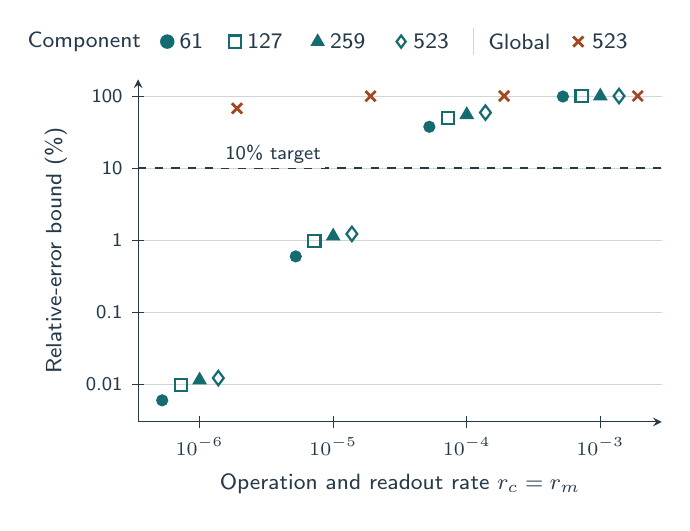
\begin{tikzpicture}[x=1cm,y=1cm,plot text]
  % Equal-rate cells from results/circuit.json at k=4, in percent.
  \pgfplotstableread{
    power comp61 comp127 comp259 comp523 global523
    -6 0.00598157 0.00974799 0.01139790 0.01217668 67.28774058
    -5 0.59458862 0.96712176 1.13372104 1.22061913 99.51258966
    -4 37.41097032 49.83892886 54.89842846 58.84804091 99.99476888
    -3 98.35530352 99.16958902 99.55646221 99.84155266 99.99994108
  }\stripratepoints
  \begin{semilogyaxis}[paper axis,at={(1.46cm,0cm)},anchor=south west,
    width=6.65cm,height=4.35cm,axis lines=left,
    xmin=-6.46,xmax=-2.54,ymin=.003,ymax=170,
    xtick={-6,-5,-4,-3},xticklabels={$10^{-6}$,$10^{-5}$,$10^{-4}$,$10^{-3}$},
    ytick={.01,.1,1,10,100},yticklabels={0.01,0.1,1,10,100},
    minor tick style={draw=none},ymajorgrids,xlabel={Operation and readout rate $r_c=r_m$},
    ylabel={Relative-error bound (\%)}]
    \draw[graphink,dashed,line width=.8pt]
      (axis cs:-6.46,10)--(axis cs:-2.54,10);
    \node[anchor=south,inner sep=1.6pt,fill=white,
          font=\sffamily\scriptsize,text=graphink]
      at (axis cs:-5.45,10) {10\% target};
    \addplot[only marks,graphteal,mark=*,mark size=2pt]
      table[x expr=\thisrow{power}-.28,y=comp61] {\stripratepoints};
    \addplot[only marks,graphteal,mark=square,mark size=2.2pt,
             mark options={solid,fill=white,line width=.8pt}]
      table[x expr=\thisrow{power}-.14,y=comp127] {\stripratepoints};
    \addplot[only marks,graphteal,mark=triangle*,mark size=2.7pt]
      table[x=power,y=comp259] {\stripratepoints};
    \addplot[only marks,graphteal,mark=diamond,mark size=2.6pt,
             mark options={solid,fill=white,line width=.8pt}]
      table[x expr=\thisrow{power}+.14,y=comp523] {\stripratepoints};
    \addplot[only marks,graphrust,mark=x,mark size=2.6pt,
             mark options={solid,line width=1pt}]
      table[x expr=\thisrow{power}+.28,y=global523] {\stripratepoints};
  \end{semilogyaxis}
  \node[anchor=west,inner sep=0pt] at (.05,4.83) {Component};
  \foreach \mx/\markshape/\qubits in {1.83/*/61,2.69/square/127,3.74/triangle*/259,4.80/diamond/523}{
    \draw[graphteal,line width=.8pt] plot[only marks,mark=\markshape,
      mark size=2.2pt] coordinates {(\mx,4.83)};
    \node[anchor=west,inner sep=0pt] at (\mx+.15,4.83) {\qubits};
  }
  \draw[graphgrid] (5.72,4.66)--(5.72,5.00);
  \node[anchor=west,inner sep=0pt] at (5.90,4.83) {Global};
  \draw[graphrust,line width=1pt] plot[only marks,mark=x,mark size=2.6pt]
    coordinates {(7.05,4.83)};
  \node[anchor=west,inner sep=0pt] at (7.22,4.83) {523};
\end{tikzpicture}
\caption{Certified relative error of the harmonic estimate of $P_{\rm sil}$
at cutoff $k=4$. Legend numbers give the data-qubit counts.
Each group is one evaluated rate with $r_m=r_c$. Symbols are offset
within a group for visibility. The four
component bounds meet the $10\%$ target at $10^{-6}$ and $10^{-5}$ and
exceed it at $10^{-4}$ and $10^{-3}$. Crosses give the global-cutoff
bound on 523 qubits ($m=48$).}
\label{fig:strip-rate-target}
\end{figure}

\begin{table}[H]
\centering\small
\setlength{\tabcolsep}{3.5pt}
\caption{Circuit component calculation at cutoff four. Building the
catalogue is a one-time cost, rounded to the nearest second here.
Evaluation time and peak memory are maxima over the eight circuit
points on each code, including catalogue loading. Jobs for distinct
points ran concurrently.}
\label{tab:strip-resources}
\smallskip
\begin{tabular}{@{}rrrr@{}}
\toprule
Qubits & Build (s) & Evaluate (s) & Peak (GiB)\\
\midrule
61  & 370  & 535    & 0.43\\
127 & 1254 & 3534   & 0.48\\
259 & 2927 & 9378   & 0.52\\
523 & 6445 & 15\,254 & 0.57\\
\bottomrule
\end{tabular}
\end{table}

The supplementary data give the complete Bernoulli grid and all circuit evaluation times.

\subsection{Rare-event comparisons on 61 and 225 qubits}\label{app:rare-methods}
Each circuit in Table~\ref{tab:rare-event-runs} was evaluated with
one rate schedule and a single-site Metropolis proposal. At each rate
the target distribution is the circuit law conditioned on silent failure.
Bennett's
acceptance ratio estimates the ratios of $P_{\rm sil}$ between
adjacent rates~\cite{Bennett76,BV13}. The first twelve silent
configurations at the high-rate anchor each started three
chains~\cite{BCCY25}. A proposal chooses a site $s$ and a different
label there, both uniformly. Under the current site law $\pi_s$, a
change $c\to c'$ is accepted with probability
$\min\{1,\pi_s(c')/\pi_s(c)\}$ if the proposed state is silent and
zero otherwise. Rejections repeat the current state. This rule preserves
the conditional law. In Fig.~\ref{fig:recomposition}, the failures in one
logical class form two disconnected components under single-site moves.

For the schedules in Table~\ref{tab:splitting-schedules}, the proposed
next operation rate is $r_c\,2^{-1/\sqrt{\max(3,h)}}$, rounded up
and bounded below by the next prescribed rate~\cite{BV13}. On the
strip $h$ is the expected number of nonzero sites. On the affine code
$h=3240r_c+108r_m$ bounds that expectation. Each chain carries its
last state into the next level. It starts with $10^5$ steps per level
and can grow to $3.1\cdot10^6$. For each adjacent ratio, let $\bar g$,
$s_g$ and $\bar g_{1/2}$ be the mean, sample standard deviation and
first-half mean of its Bennett statistic after $T$ steps. A chain
extends when $\max_g[s_g/(\sqrt{T}\,\bar g)]+
\max_g[|\bar g_{1/2}-\bar g|/\bar g]$ exceeds $0.05/\sqrt{J}$,
with each maximum taken over the adjacent ratios~\cite{BCCY25}.

On 61 qubits, anchor sampling stopped at the $2\,010$th silent
history. A separate direct run at $r_c=r_m=10^{-3}$ recorded 477
silent failures in $7\cdot10^9$ rounds. On 225 qubits a calibration
batch of $250\,000$ histories set the independent anchor sample size
at $2\cdot10^8$, with 574 silent failures. At the final level, 10 of
the 36 chains accounted for all 26 state changes over $3.6\cdot10^6$
steps. The other 26 chains never moved.

Mayer et al.\ used splitting on rotated surface codes to estimate
logical failure below $10^{-20}$~\cite[Sec.~6.2]{Mayer26}. Smith,
Brown and Bartlett run splitting separately in each accepted logical
sector of a surface code and normalize the estimates to obtain the
conditional failure probability~\cite{SBB24}. Other kernels resample
subregions~\cite{MWB26} or exchange clusters~\cite{HM26}.

\begin{table}[H]
\centering\small
\setlength{\tabcolsep}{3pt}
\caption{Rare-event runs with the prescribed SSF. The strip entry
gives the result at $r_c=r_m=10^{-5}$ and its deterministic reference.
Its time covers the full run at four rates. The affine circuit uses
VV first at $(r_c,r_m)=(2\cdot10^{-7},10^{-5})$, with the reference
coverage of Table~\ref{tab:affine225-pilot}. The last row samples the
two-data, one-readout stratum at $(p,q)=(10^{-6},10^{-4})$ with a
prepared decoder.}
\label{tab:rare-event-runs}
\smallskip
\begin{tabular}{@{}lrr@{}}
\toprule
Estimate & Reference & Time\\
\midrule
\multicolumn{3}{@{}l}{61-qubit strip, circuit splitting ($P_{\rm sil}$)}\\
$1.10704\cdot10^{-13}$ & $[8.1358,8.2332]\cdot10^{-14}$ & 2.49 h\\
\addlinespace
\multicolumn{3}{@{}l}{225-qubit affine code, circuit splitting ($P_{\rm sil}$)}\\
$4.91234\cdot10^{-16}$ & $[3.33938,3.34508]\cdot10^{-16}$ & 161.91 s\\
\addlinespace
\multicolumn{3}{@{}l}{225-qubit affine code, Bernoulli subset sampling ($f_{21}$)}\\
$119/10^6$ & $324/2\,721\,600=1/8400$ & 0.345 s\\
\bottomrule
\end{tabular}
\end{table}

\begin{table}[H]
\centering\small
\setlength{\tabcolsep}{3pt}
\caption{Splitting rate schedules. The strip sequence includes every
decade between its endpoints. On the affine code $r_c=10^{-4}$ is
an intermediate level.}
\label{tab:splitting-schedules}
\smallskip
\begin{tabular}{@{}lcc@{}}
\toprule
 & 61-qubit strip & 225-qubit code\\
\midrule
Anchor $r_c$       & $10^{-2}$ & $3\cdot10^{-3}$\\
Readout $r_m$      & $r_c$ & $\min(0.005,50r_c)$\\
Lowest $r_c$       & $10^{-6}$ & $2\cdot10^{-7}$\\
Rate levels $J$    & 25 & 28\\
Effective sites    & 91 & 333\\
\bottomrule
\end{tabular}
\end{table}

Multiparameter subset sampling weights each vector of fault counts by
its product of binomial masses~\cite[Eq.~(10)]{GMB19}. Here $w_{ab}$ is
the Bernoulli mass of $a$ data errors and $b$ readout flips, and $f_{ab}$
is the conditional silent-failure probability within that stratum. For
independent samples of fixed sizes $N_{ab}$ with replacement,
the weighted sum has exact variance
\[
 \sum_{(a,b)\ {\rm retained}}
       w_{ab}^{\,2}\frac{f_{ab}(1-f_{ab})}{N_{ab}} .
\]
At $(p,q)=(10^{-6},10^{-4})$,
$S=\binom{225}{2}108=2\,721\,600$
and $w_{21}=S p^2(1-p)^{223}q(1-q)^{107}$.
The $324$ silent configurations give $f_{21}=1/8400$ and
$w_{21}f_{21}\simeq3.20480\cdot10^{-14}$. The relative variance of
the stratum estimate is $8399/N_{21}$, giving the normal planning estimate
$N_{21}\simeq z_{0.975}^2\,8399/\epsilon^2$, about $3.23\cdot10^6$
or $3.23\cdot10^8$ draws for nominal $95\%$ relative half-widths
of $10\%$ or $1\%$. Uniform sampling without replacement multiplies
the variance by $(S-N_{21})/(S-1)$, reaching zero at the census.

For the sampled Bernoulli stratum the two-sided $95\%$
Clopper--Pearson interval~\cite{Clopper34} for $f_{21}$ was
$[0.98582,1.42400]\cdot10^{-4}$ (rounded outward). With the same
precomputed tables, sampling and exact counting took $0.345$ and
$0.795$ s, including decoder loading and checks. Building the tables
took $1.535$ s. The circuit sector timing in
Section~\ref{sec:finite-estimates} includes setup.

\raggedend
\section{Numerical data and code}\label{app:support}
\begingroup\raggedright
Version~2 of the reproduction package is archived on Zenodo
(DOI \href{https://doi.org/10.5281/zenodo.24521353}{\nolinkurl{10.5281/zenodo.24521353}}).
The source repository is
\url{https://github.com/vicenzoscavino1999/ssf-qec-reproduction}.
After extracting \path{REPRODUCCION_SSF_QEC_20261124.zip}, run
\mbox{\texttt{py -3.12 reproducir.py rapido}} in PowerShell from the
package root. This verifies the file hashes and recomputes the Bernoulli
intervals in Table~\ref{tab:two-volumes} from the archived counts.
The guide \href{https://zenodo.org/records/24521353/files/REPRODUCTION.md?download=1}{\nolinkurl{REPRODUCTION.md}}
lists the archive paths and reproduction commands for the supplements below.

\paragraph{Uniform rates.}
\path{SOURCE_CUMULANT_CERTIFICATE.zip} gives the derivation of
\eqref{eq:mixed-source-row} and its rational verifier \path{verify.py}.
\path{FIBRE_CERTIFICATES.zip} supplies the degree-specific proofs,
the rate verifiers indexed by noise model and schedule, and
\path{verify_first_contact.py} for the counterexamples in
Appendix~\ref{app:contact-examples}.

\paragraph{Affine F17.}
\path{REPRODUCCION_PAPER_20261117_v3.zip} supplies the mask and
competition calculations in \path{supplement/h1/} and
\path{supplement/h3/}. \path{F17_CIRCUIT_SECTOR_20261107.zip}
contains the point--line data for~\eqref{eq:finite-anchor}.

\paragraph{Finite codes.}
\path{reproducir.py} in \path{SSF_SECTORES_225_900_20261124.zip}
rebuilds Table~\ref{tab:two-volumes} and the two intervals in
Fig.~\ref{fig:affine-estimates}(b) from the seeds. The direct 900-qubit
census is recorded in \path{referencia/directo_900.txt}.
\path{HGP225_PILOT.zip} gives the stratum counts for
Table~\ref{tab:affine225-pilot} and the independent implementation
\path{auditar_esquinas_HGP_225.py}.
\path{QEC_RARE_EVENT_COMPARISONS_20261124.zip} gives
the circuit estimates in Figs.~\ref{fig:affine-estimates}(a)
and~\ref{fig:strip-comparison}(b). Its files \path{RESULTADO_T2_2.json}
and \path{resultado_splitting.json} give every rate and the per-level
chain diagnostics for 61 and 225 qubits, respectively.
The PATH25 syndrome enumeration is in \path{PATH25_VALIDATION_20261106.zip}.
The circuit enumeration and cutoff-eight calculation in
Appendix~\ref{app:strip-certificates} are in
\path{PATH25_CERTIFIED_ESTIMATORS_20261112.zip}.
For the strips,
\path{STRIP_COMPONENT_CERTIFICATES_20261116.zip} supplies endpoints
and \path{reproduce_tables.py}. Its \path{results/circuit.json} gives the bounds
plotted in Figs.~\ref{fig:strip-comparison}(a) and~\ref{fig:strip-rate-target}. The catalogue inputs are in
\path{T2_1_REPRODUCCION_COMPLETA_20261116.zip}.
\par\endgroup

\end{document}
